%.$ xelatex --shell-escape TP1.tex

%path to figures
\newcommand{\figures}{./Figures}

\documentclass[
11pt,
oneside,
french,
singlespacing,
liststotoc,
toctotoc,
headsepline,
]{MastersDoctoralThesis}

\usepackage{mathpazo}
\usepackage{fontspec}
\setmainfont[Ligatures=TeX, Mapping=tex-text]{TeX Gyre Pagella}
\setmonofont{FreeMonoBold}
\usepackage[backend=bibtex, style=authoryear, natbib=true]{biblatex}
\addbibresource{example.bib}
\usepackage[autostyle=true]{csquotes}
\usepackage{enumitem}
\usepackage{float}
\usepackage{amsmath}
\usepackage{minted}
\usepackage{xcolor}

\geometry{
	paper=a4paper,
	inner=2.5cm,
	outer=2.5cm,
	bindingoffset=0.5cm,
	top=1.5cm,
	bottom=1.5cm,
	}

\thesistitle{Autoscope\\Compte rendu final}
\supervisor {}
\examiner{}
\degree{\href{http://www.estei.fr/filiere/informatique-systemes-embarques}{MASTER Systèmes Embarqués}}
\author{Thomas ABGRALL\\Clément AILLOUD\\Thibaud LE DOLEDEC\\\href{https://www.github.com/thomaslepoix}{Thomas LEPOIX}}
\addresses{}
\subject{}
\keywords{}
\university{\href{http://www.estei.fr}{E.S.T.E.I.}}
\department{\href{http://www.estei.fr}{École Supérieure des Technologies Électronique, Informatique, et Infographie}}
\group{\href{http://www.estei.fr/filiere/informatique-systemes-embarques}{Département Systèmes Embarqués}}
\faculty{\href{http://www.estei.fr}{E.S.T.E.I.}}

\AtBeginDocument{
	\hypersetup{pdftitle=\ttitle}
	\hypersetup{pdfauthor=\authorname}
	\hypersetup{pdfkeywords=\keywordnames}
	}

\begin{document}

\mainmatter
\pagestyle{plain}
\usemintedstyle{monokailight}
%bash/Ruby/basemake/
\definecolor{gris}{gray}{0.97}
\definecolor{gris2}{HTML}{282828}
\definecolor{ubuntu}{HTML}{300A24}

\newcommand{\code}[1]{\begin{minted}[
linenos,
breaklines,
breakautoindent,
breakaftersymbolpost,
bgcolor=gris,
fontsize=\scriptsize,
obeytabs,
tabsize=4,
showtabs,
]{#1}}

\newcommand{\codeinline}[2]{\mintinline[fontsize=\footnotesize]{#1}{#2}}


%------------------------------------------------------------------

\begin{titlepage}
\begin{center}

{\href{http://www.estei.fr}{
\includegraphics[width=\linewidth]{\figures/estei.png}}}
\vspace*{.06\textheight}
\vspace{1.5cm}\\
\textsc{\Large Projet de MASTER 2}\\[0.5cm]

\HRule \\[0.4cm]
{\huge \bfseries \ttitle\par}\vspace{0.4cm}
\HRule \\[1.5cm]

\large{\emph{Auteurs :}\\
\authorname}

\vspace{4cm}
\degreename\\[1cm]
{\vspace{0.4cm}\scshape\LARGE \univname}\\\deptname\\\groupname\\[1cm]

\vfill

{\large \today}\\[1cm]

\end{center}
\end{titlepage}

%------------------------------------------------------------------

%\begin{acknowledgements}
%\addchaptertocentry{\acknowledgementname} % Add the acknowledgements to the table of contents
%\end{acknowledgements}

\tableofcontents

\pagestyle{thesis}

%chapter Cahier des charges
%chapter Structure 3D
%chapter Hardware
%chapter Middleware
%chapter Software
%chapter Conclusion

\part{Partie de groupe}
\chapter{Avancement général}

En raison de l'abandon du projet par Thibaud LE DOLEDEC et Clément AILLOUD partis en stage, le projet ne pourra être mené à terme. Pour aborder la dernière ligne droite avant l'évaluation finale, un choix a donc été fait des taches sur lesquelles travailler en priorité, au détriment d'autres qui demeureront inachevées.

\vspace{1cm}

Ci-dessous un diagramme représentant l’avancement des différentes taches du projet. Le gris indique qu’une tache est terminée ou à un niveau d’avancement satisfaisant et garantissant une maturité proche. Le orange indique les taches sur lesquelles nous travaillerons en priorité avant la fin du projet. Les flèches représentent des liens de dépendance entre les taches.

\begin{figure}[H]
    \centering
	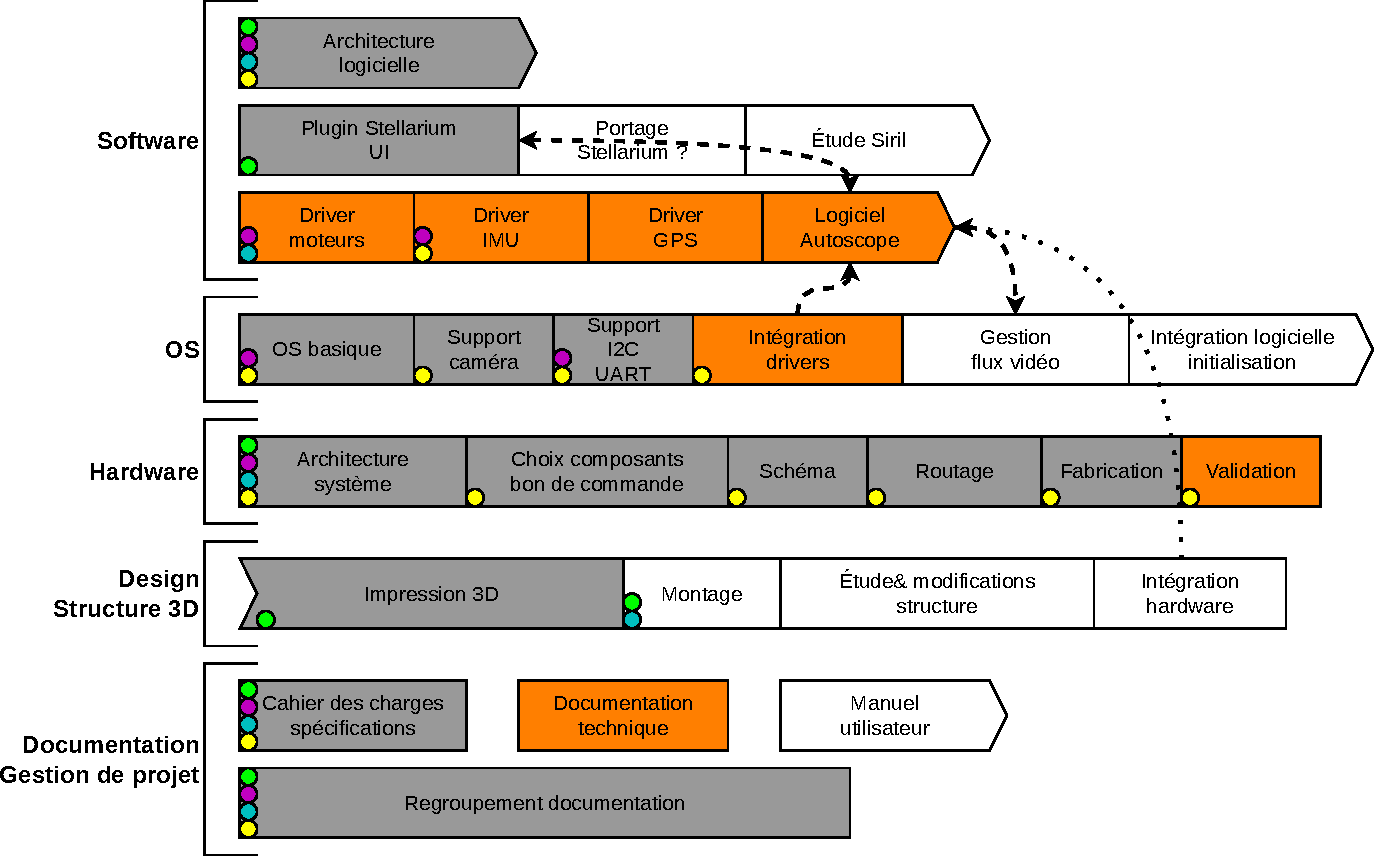
\includegraphics[width=1\linewidth]{\figures/sch_gantt.pdf}
    \decoRule
    \caption[
    Diagramme de l'organisation temporelle du travail sur le projet]{
    Diagramme de l'organisation temporelle du travail sur le projet}
    \label{fig:Diagramme de l'organisation temporelle du travail sur le projet}
    \end{figure}

\section{Prévisions pour le dernier sprint}

Malgré son aspect visuel intéressant pour promouvoir le projet ainsi que de sont aspect central (il s'agit tout de même d'un télescope), le travail sur la structure du télescope sera écarté des taches prioritaires. Cela pour deux raisons~:
\begin{itemize}[label=$\bullet$]
	\item Il s'agit d'une partie du projet demandant beaucoup de temps et d'implications par rapport à ce dont nous disposons. Nous n'aurions sans doute pas le temps de terminer cela avant l'évaluation.
	\item N'ayant ni des connaissances particulières en optique, ni la maîtrise d'un logiciel de modélisation 3D, nous ne sommes pas plus qualifiés qu'une personne aléatoire voulant contribuer au projet. Nous pensons donc qu'il vaut mieux nous concentrer sur des taches faisant partie de notre domaine de qualification, que nous serions capable de réaliser plus facilement ou mieux qu'une personne aléatoire. L'élaboration des drivers correspond typiquement à ce cas.
	\end{itemize}

\vspace{1cm}

Le travail sur les drivers, quant à lui devra être avancé autant que faire se peut. En effet le logiciel principal du télescope dépend lourdement des interfaces avec les drivers et ne peut être commencé tant que les drivers ne sont pas fonctionnels.

De plus, ce logiciel étant la clef de voûte du projet, la finalisation de certaines taches comme certains éléments du plugin Stellarium ou la gestion du flux vidéo au sein de l'OS doit être réalisée conjointement à l'écriture de ce logiciel.

L'absence des ces drivers commence donc à bloquer l'évolution d'autres taches.

\vspace{1cm}

Enfin un travail de documentation devra être fait pour qu'il soit possible à une personne future (nous-mêmes ou qui que ce soit) de travailler sur ce projet ou de réutiliser notre travail.





\chapter{Accessibilité au projet sur internet}

Le projet étant libre, il est disponible sur Github sous licence GPL-2. Nous tachons d'accompagner nos différents dépôts d'une documentation claire permettant d'obtenir les informations suivantes~:
\begin{itemize}[label=$\bullet$]
	\item Une description brève et précise sur le contenu du dépôt et son rôle au sein du projet.
	\item Une explication de la procédure à suivre pour utiliser le contenu du dépôt.
	\item Une explication de la procédure à suivre pour travailler sur le dépôt.
	\end{itemize}

\section{Dépôt principal}

\url{https://github.com/thibaudledo/Autoscope}

\vspace{1cm}

Le dépôt est organisé comme suit~:
\begin{itemize}[label=$\bullet$]
	\item Branche {\href{https://github.com/thibaudledo/Autoscope/tree/master}{\codeinline{text}{master}}}~: Licence du projet et explications sur le projet dans son ensemble.
	\item Release {\href{https://github.com/thibaudledo/Autoscope/releases}{\codeinline{text}{alpha}}}~: Paquets et fichiers binaires pour utiliser le projet "out of the box" (release expérimentale).
	\item Branche {\href{https://github.com/thibaudledo/Autoscope/tree/hardware}{\codeinline{text}{hardware}}}~: Fichiers Blender de la structure du télescope et fichiers KiCad de la carte électronique du projet.
	\item Branche {\href{https://github.com/thibaudledo/Autoscope/tree/doc}{\codeinline{text}{doc}}}~: Documentations et datasheets des composants et éléments utilisés pour le projet.
	\item Branche {\href{https://github.com/thibaudledo/Autoscope/tree/latex}{\codeinline{text}{latex}}}~: Fichiers LaTex et \codeinline{text}{.pdf} des comptes rendus sur le projet.
	\item Branche {\href{https://github.com/thibaudledo/Autoscope/tree/hello_mod}{\codeinline{text}{hello_mod}}}~: Sources d'un driver helloworld servant d'exemple.
	\item Branche {\href{https://github.com/thibaudledo/Autoscope/tree/a4988_mod}{\codeinline{text}{a4988_mod}}}~: Sources du driver des contrôleurs moteur et des capteurs de fin de course des moteurs.
	\item Branche {\href{https://github.com/thibaudledo/Autoscope/tree/mpu_9250_mod}{\codeinline{text}{mpu_9250_mod}}}~: Sources du driver de la centrale inertielle.
	\item Branche {\href{https://github.com/thibaudledo/Autoscope/tree/mtk3339_mod}{\codeinline{text}{mtk3339_mod}}}~: Sources du driver du GPS.
	\end{itemize}

\newpage
\section{Dépôt du système d'exploitation de la Raspberry-Pi}

\url{https://github.com/thomaslepoix/meta-autoscope}

\vspace{1cm}

Il s'agit de la couche de métadonnées utilisées par Yocto pour construire le système d'exploitation Linux utilisé par la Raspberry-Pi du télescope. Une image pré-compilée du système d'exploitation figurera sur {\href{https://github.com/thibaudledo/Autoscope/releases}{la release \codeinline{text}{alpha} du dépôt principal}.

\vspace{1cm}

Le dépôt est organisé comme suit~:
\begin{itemize}[label=$\bullet$]
	\item Branche {\href{https://github.com/thomaslepoix/meta-autoscope/tree/rpi}{\codeinline{text}{rpi}}}~: Métadonnées Yocto et explications de comment compiler et installer le système d'exploitation.
	\item Branche {\href{https://github.com/thomaslepoix/meta-autoscope/tree/rpi-repo}{\codeinline{text}{rpi-repo}}}~: Données utilisées par Repo pour synchroniser le dépôt à d'autres dépôts de métadonnées Yocto utilisées pout construire l'OS.
	\end{itemize}

\section{Dépôt du plugin de Stellarium}

\url{https://github.com/thibaudledo/Autoscope-Stellarium-plugin}

\vspace{1cm}

Il s'agit du plugin de Stellarium contenant l'interface par laquelle l'utilisateur interagira avec le télescope. Un paquet pré-compilé pour linux de Stellarium incluant le plugin figure sur {\href{https://github.com/thibaudledo/Autoscope/releases}{la release \codeinline{text}{alpha} du dépôt principal}.

\vspace{1cm}

Le dépôt est organisé comme suit~:
\begin{itemize}[label=$\bullet$]
	\item Branche {\href{https://github.com/thibaudledo/Autoscope-Stellarium-plugin/tree/master}{\codeinline{text}{master}}}~: Sources du plugin, patch des sources de Stellarium et explications de comment compiler une version de Stellarium intégrant le plugin.
	\end{itemize}


\chapter{Structure du télescope}

\section{Projet d'origine}

La structure du télescope est imprimable à l'imprimante 3D et provient d'un projet open source entre temps disparu d'internet~:
\url{https://blog.dagoma.fr/telescope-imprime-en-3d/}

\vspace{1cm}

Voici l'allure du télescope monté. Les barres métalliques raccordant le support du miroir secondaire au reste du télescope sont des barres de camping achetées en magasin de sport.

\begin{figure}[H]
    \centering
    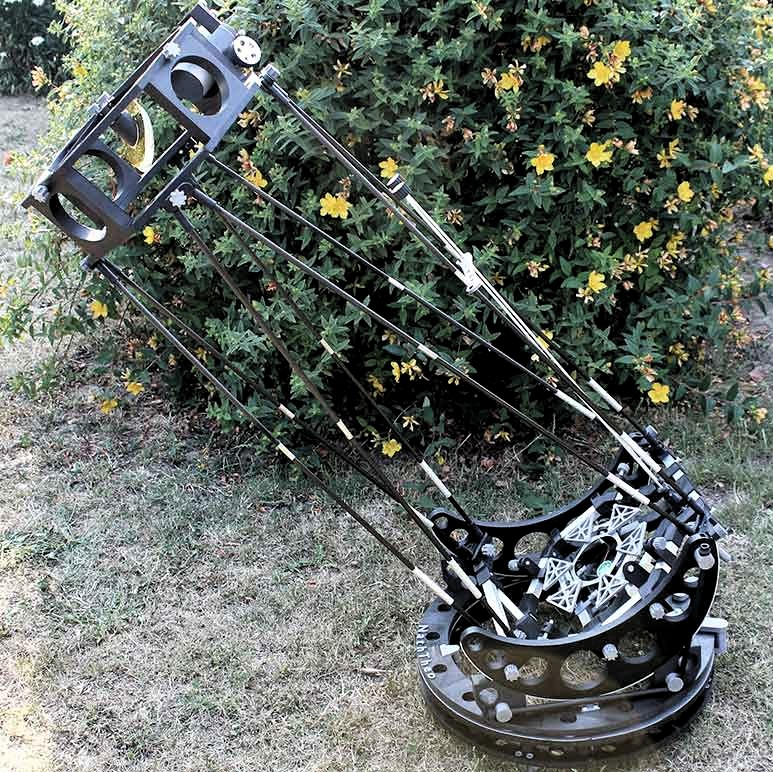
\includegraphics[width=0.5\linewidth]{\figures/photo_telescope2.jpg}
    \decoRule
    \caption[
    Photo du télescope]{
    Photo du télescope}
    \label{fig:Photo du télescope}
    \end{figure}

\begin{figure}[H]
    \centering
    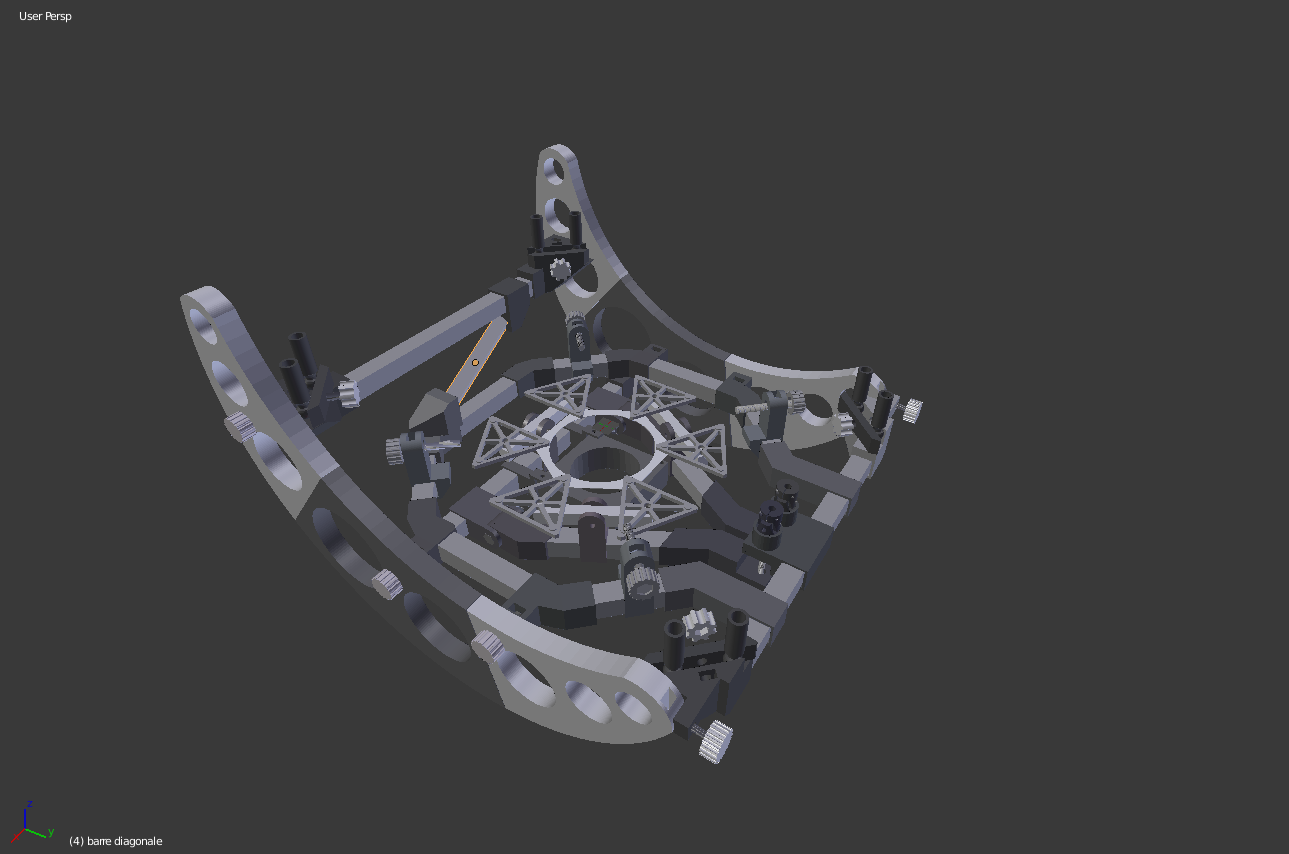
\includegraphics[width=0.49\linewidth]{\figures/blender_3.png}
    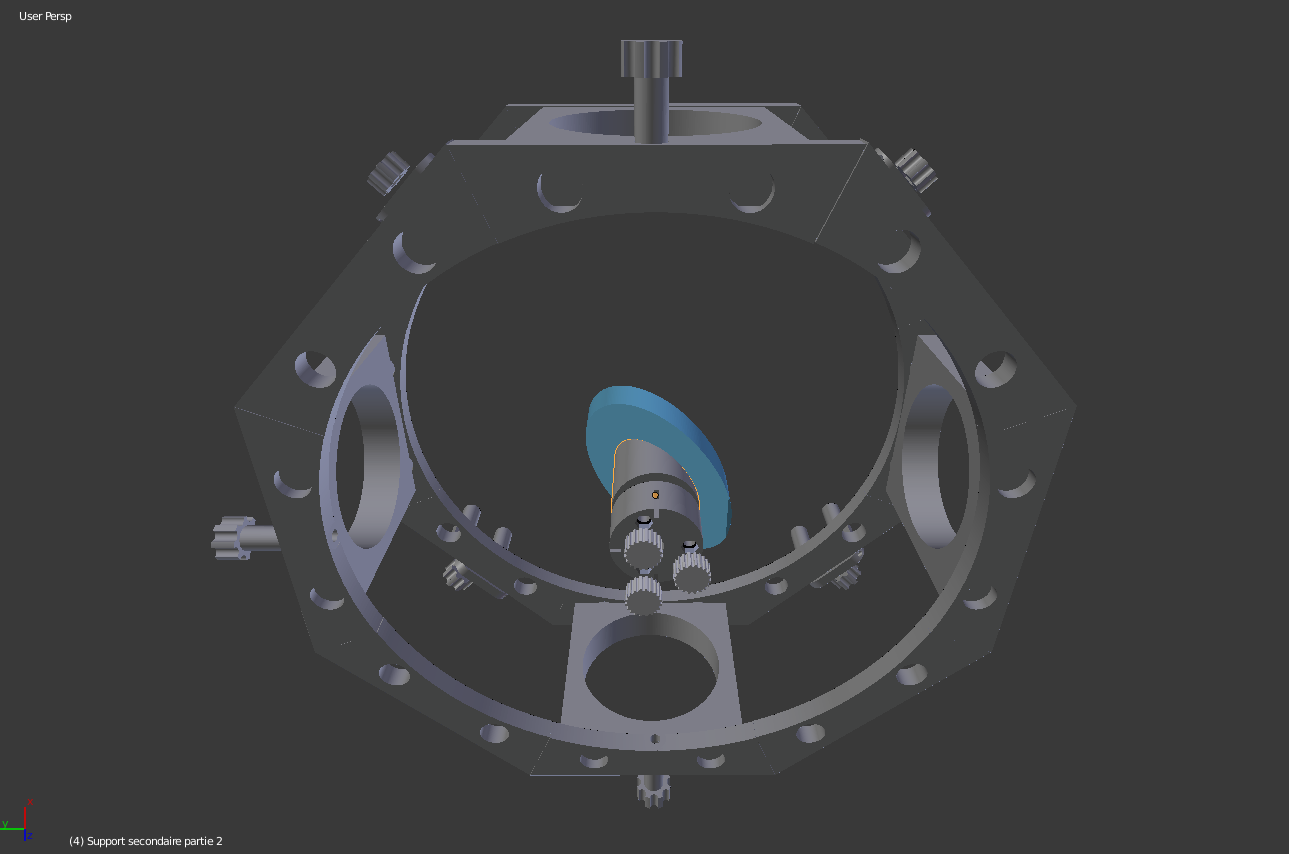
\includegraphics[width=0.49\linewidth]{\figures/blender_4.png}
    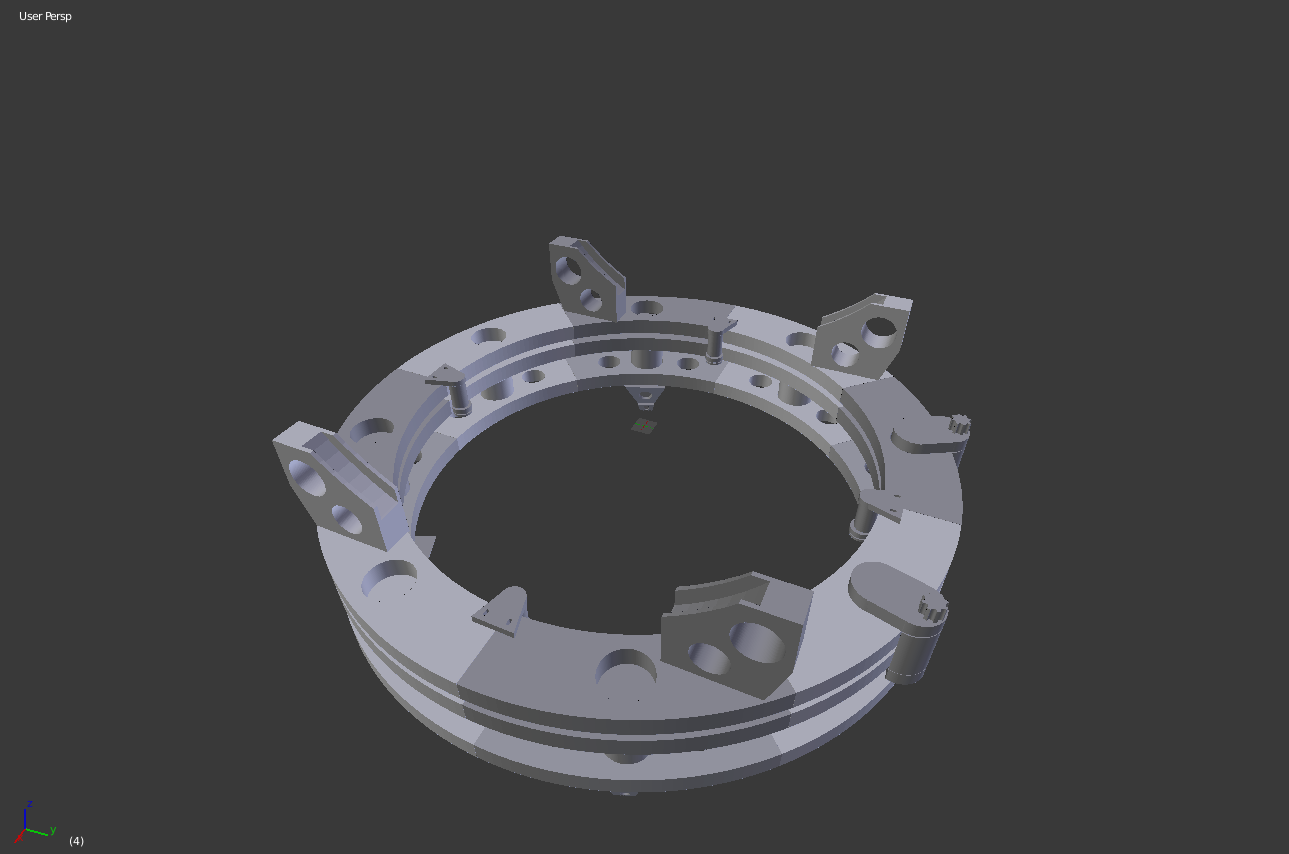
\includegraphics[width=0.49\linewidth]{\figures/blender_5.png}
    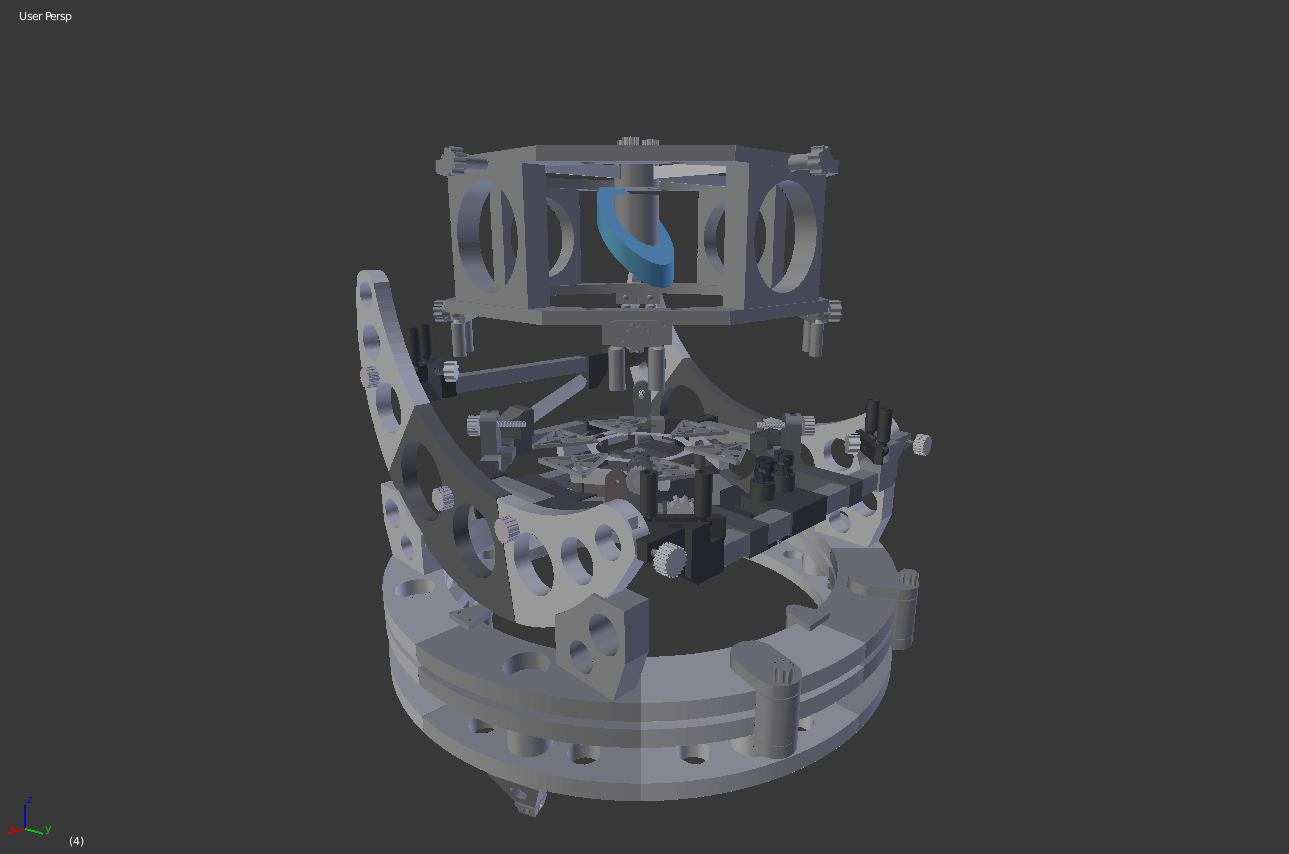
\includegraphics[width=0.49\linewidth]{\figures/blender_6.png}
    \decoRule
    \caption[
    Aperçu des fichiers de production du télescope]{
    Aperçu des fichiers de production du télescope}
    \label{fig:Aperçu des fichiers de production du télescope}
    \end{figure}

\section{Étude de la robotisation du télescope}

Ci-dessous quelques schémas représentant les modifications, telles qu'imaginées, à apporter à la structure du télescope pour l'automatiser.

\vspace{1cm}

Le socle, immobile, sera doté d'une courroie ainsi que d'un cran permettant d'activer le capteur de position. Le système électronique sera solidaire du support du miroir primaire, mobile, à l'étage supérieur. Un moteur doté d'une roue crantée fixé sur la plateforme tournante permettra de la mettre en mouvement par rapport au socle.

\begin{figure}[H]
    \centering
    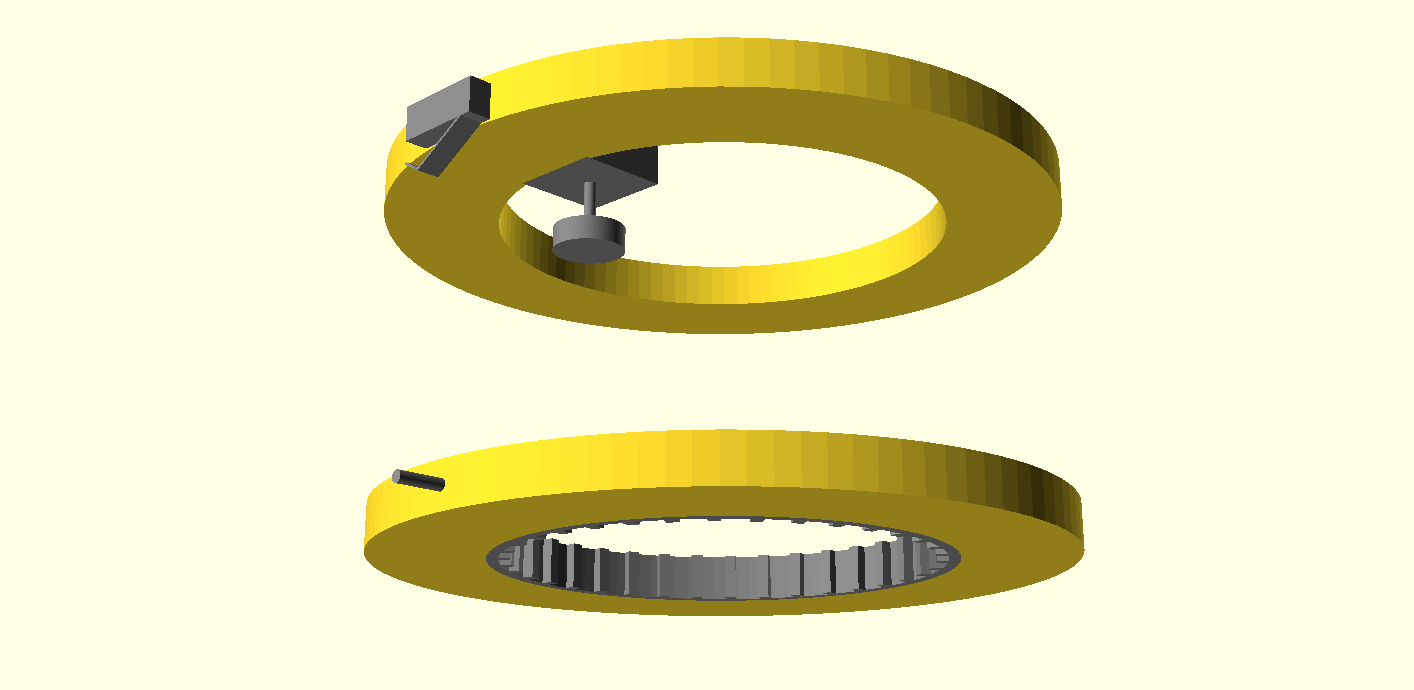
\includegraphics[width=0.9\linewidth]{\figures/OpenSCAD/azim.png}
    \decoRule
    \caption[
    Schéma du mécanisme permettant un mouvement azimutal]{
    Schéma du mécanisme permettant un mouvement azimutal}
    \label{fig:Schéma du mécanisme permettant un mouvement azimutal}
    \end{figure}

\vspace{1cm}

Pour le mouvement d'élévation, un système de tringlerie et de courroie a été imaginé pour mouvoir le support du miroir primaire par rapport à la plateforme tournante. Deux capteurs de position judicieusement placés permettront de détecter lorsque le mouvement atteint l'un de ses maximums.

\begin{figure}[H]
    \centering
    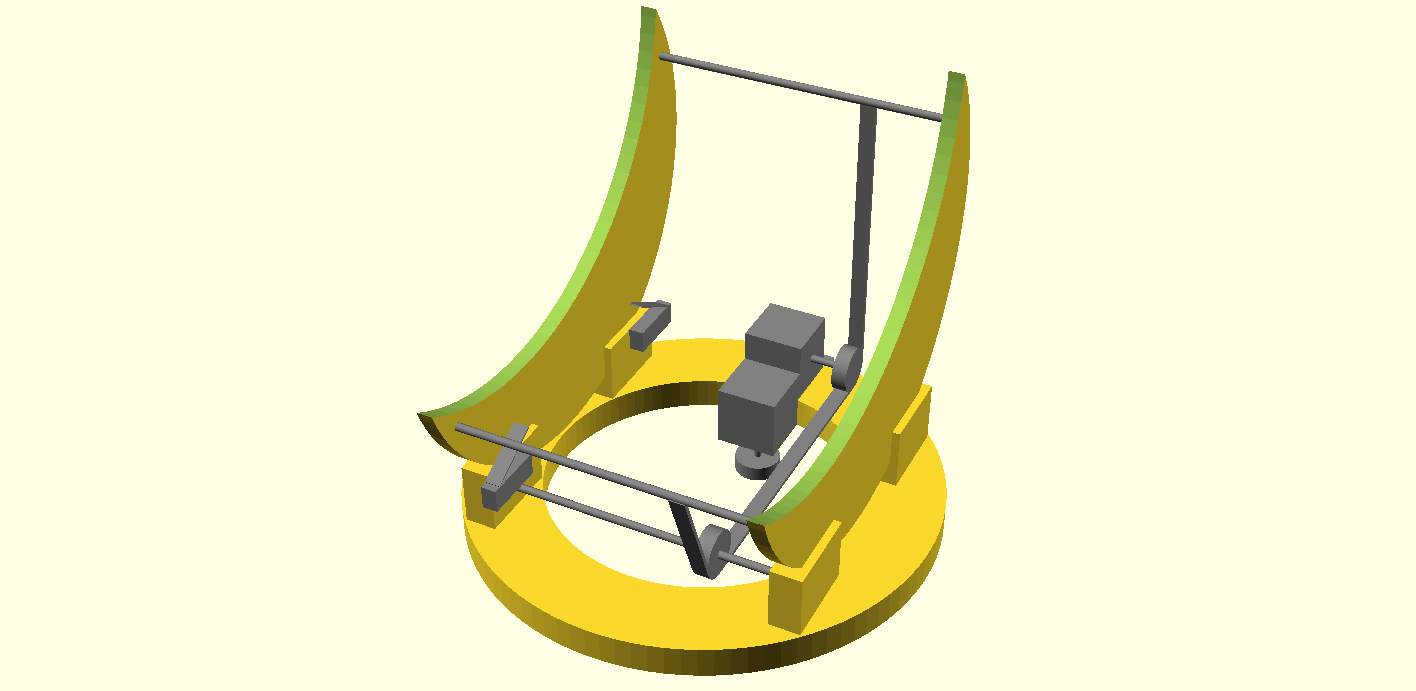
\includegraphics[width=0.9\linewidth]{\figures/OpenSCAD/elev3.png}
    \decoRule
    \caption[
    Schéma du mécanisme permettant un mouvement d'élévation]{
    Schéma du mécanisme permettant un mouvement d'élévation}
    \label{fig:Schéma du mécanisme permettant un mouvement d'élévation}
    \end{figure}

\vspace{1cm}

Quant au zoom, il faudra créer un ensemble de pièces pour maintenir le zoom lui même, la caméra (non représentée), le moteur permettant d'actionner le zoom, les capteurs de positions extrêmes, ainsi qu'un système permettant de régler finement la position de l'oculaire et de la caméra.

Un cran pour activer les capteurs de positions extrêmes pourrait être fixé à l'oculaire avec un collier de serrage par exemple.

\begin{figure}[H]
    \centering
    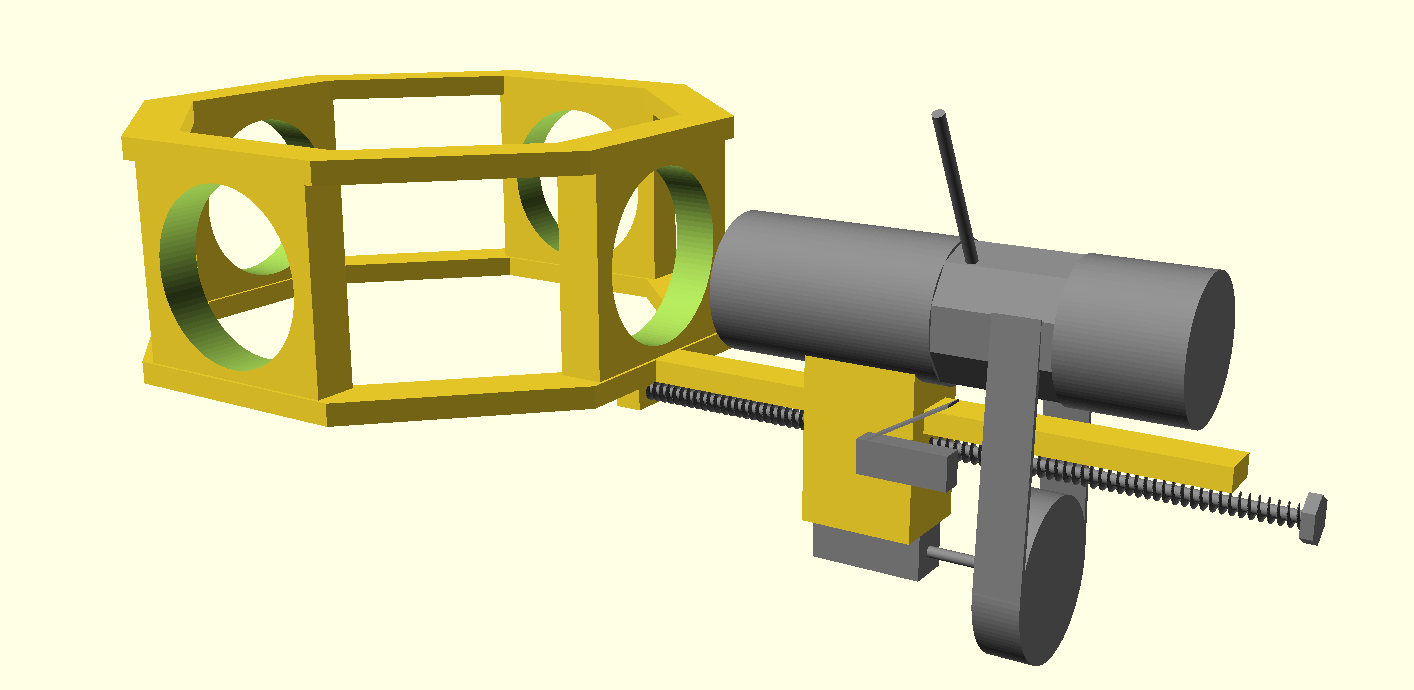
\includegraphics[width=0.9\linewidth]{\figures/OpenSCAD/zoom.png}
    \decoRule
    \caption[
    Schéma du mécanisme permettant un mouvement du zoom]{
    Schéma du mécanisme permettant un mouvement du zoom}
    \label{fig:Schéma du mécanisme permettant un mouvement du zoom}
    \end{figure}

\section{État actuel de la structure}

Pour l'instant nous avons imprimé toutes les pièces fournies par le projet original. Certaines ont subi une détérioration de la qualité lors de l'impression pour une raison mal connue et demeurent à réimprimer. Le Socle, la plateforme tournante et le support du miroir secondaire ont été montés. Aucune modification de la structure en vue d'y intégrer le système électronique n'a été faite.

\begin{figure}[H]
    \centering
    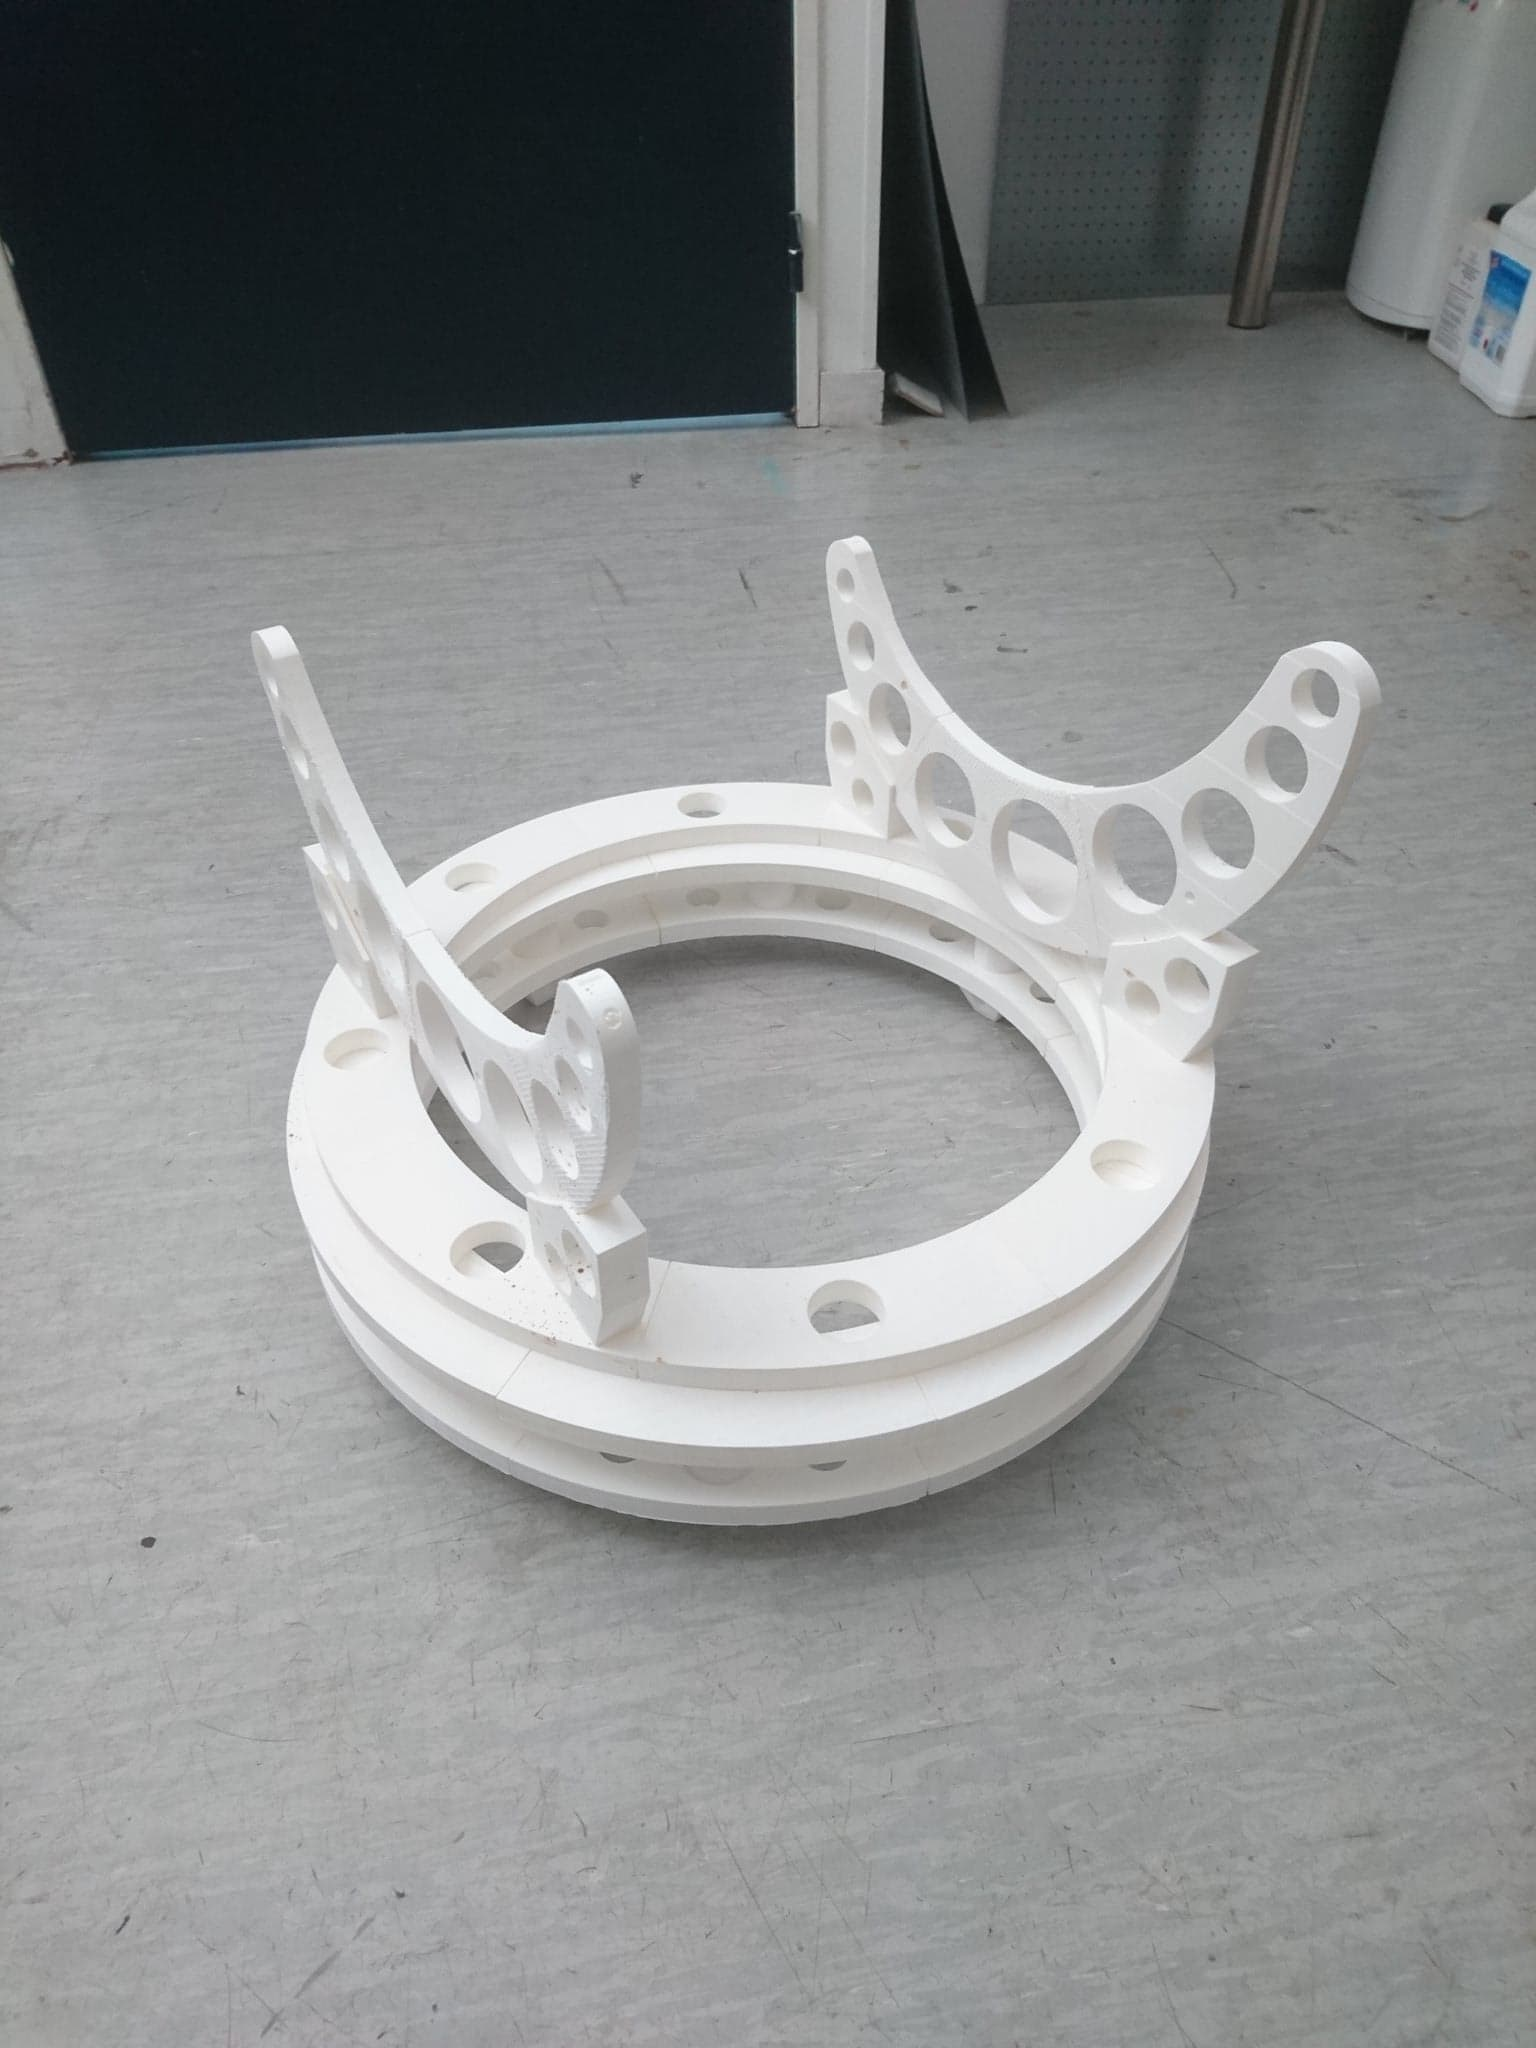
\includegraphics[width=0.3\linewidth]{\figures/photo_structure1.jpg}
    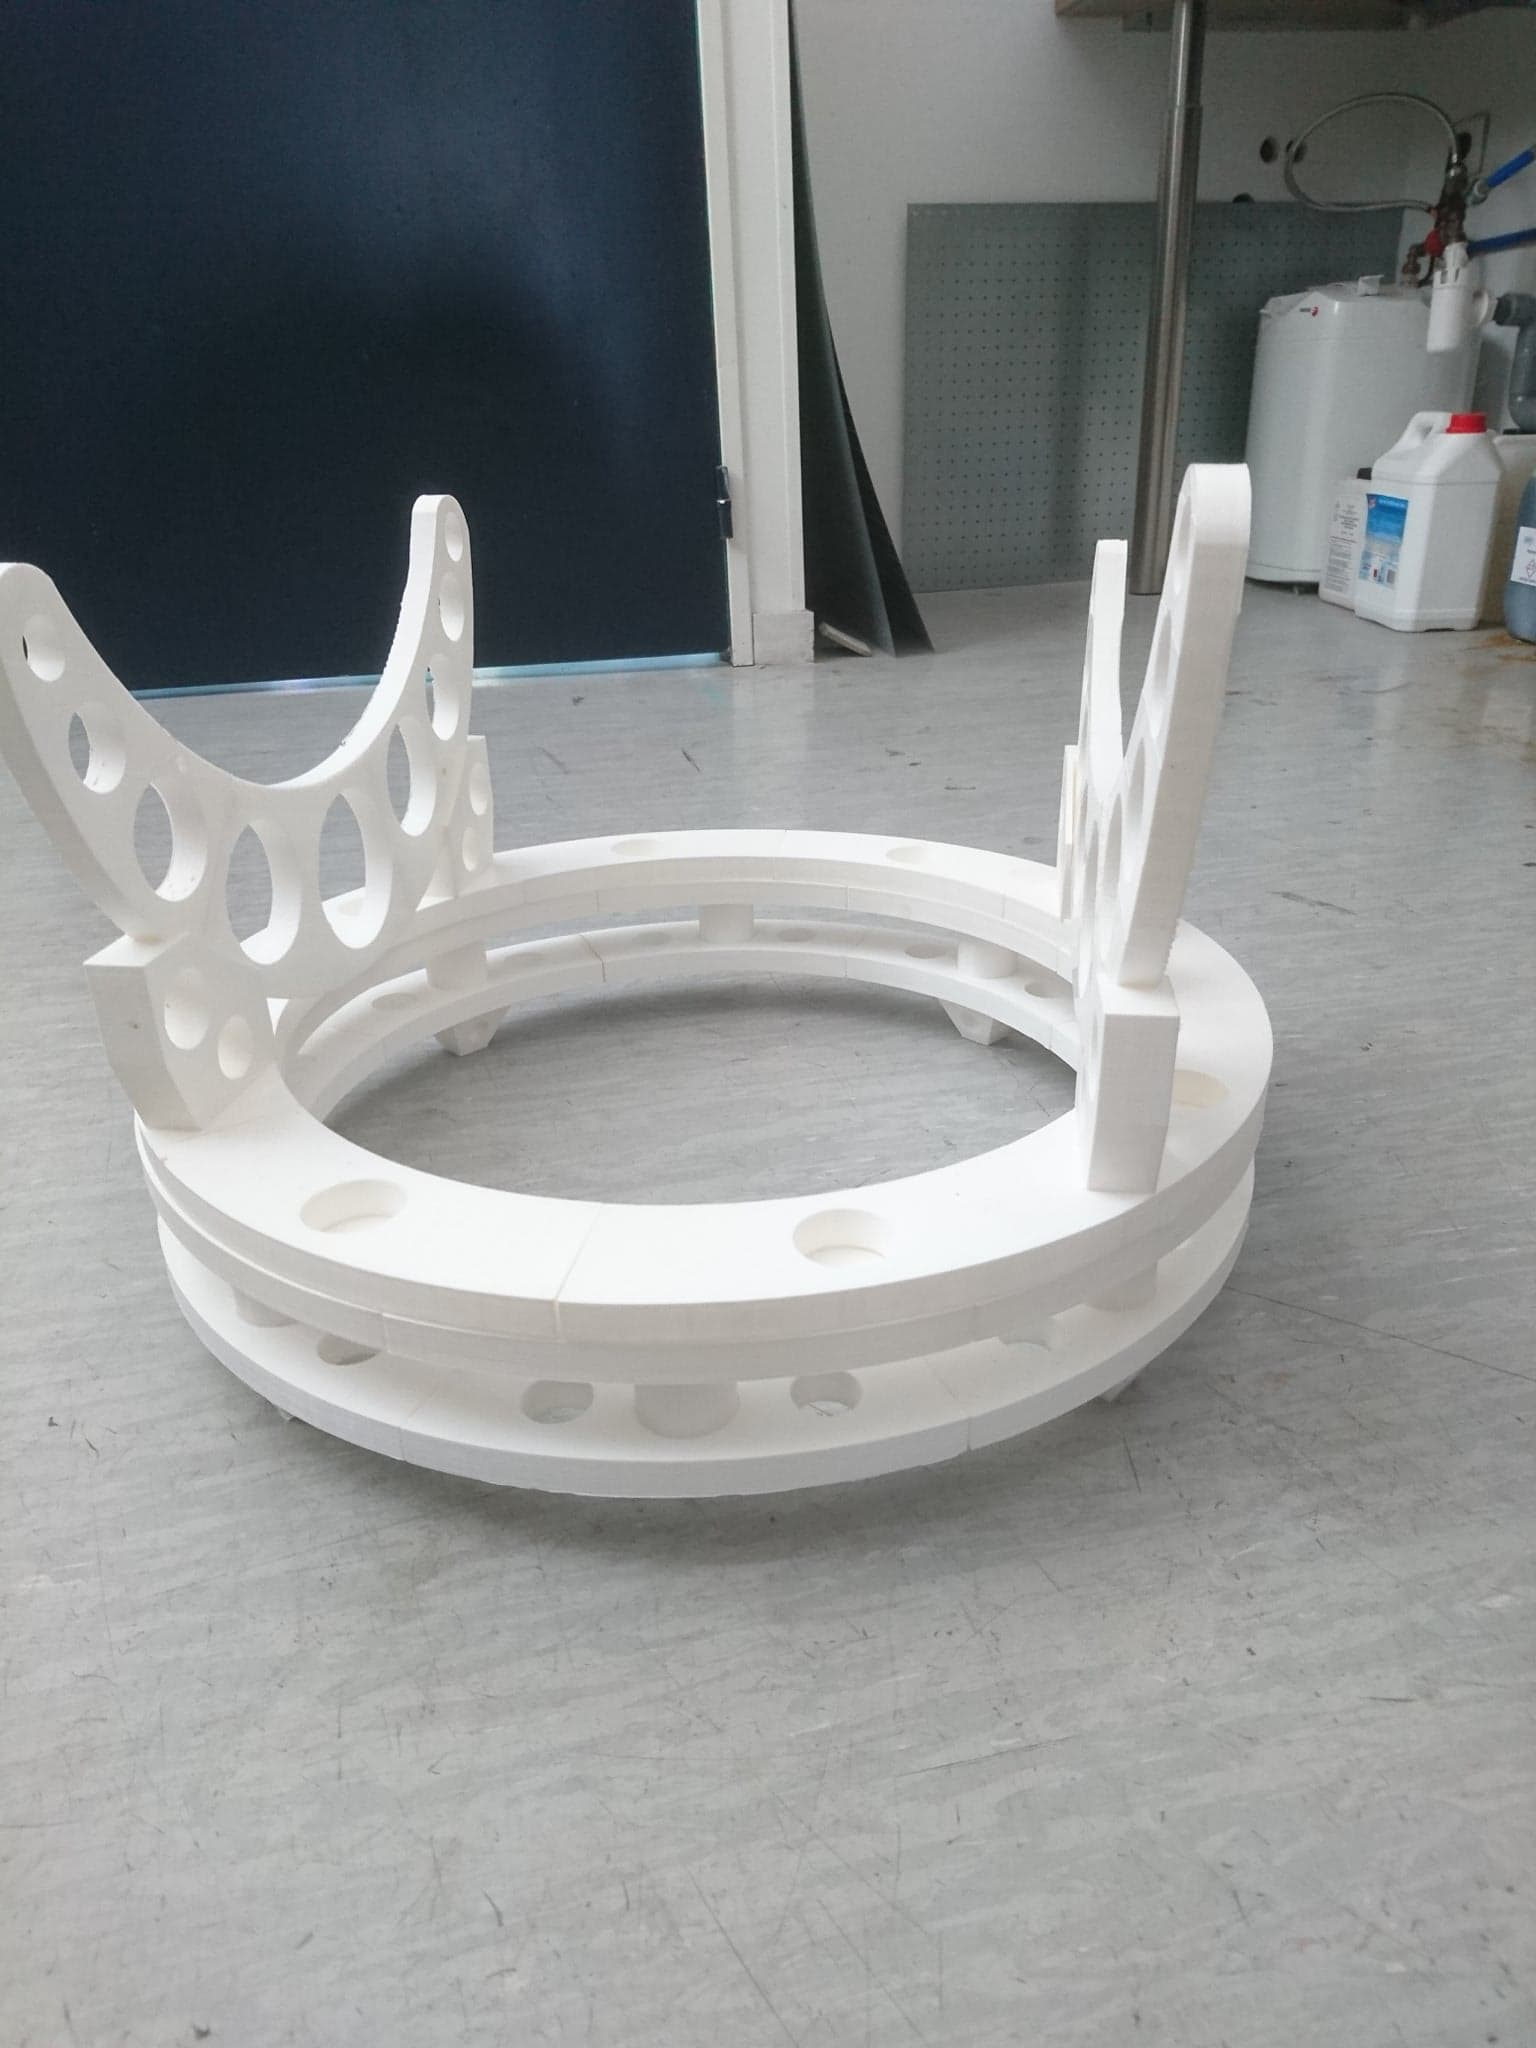
\includegraphics[width=0.3\linewidth]{\figures/photo_structure2.jpg}
    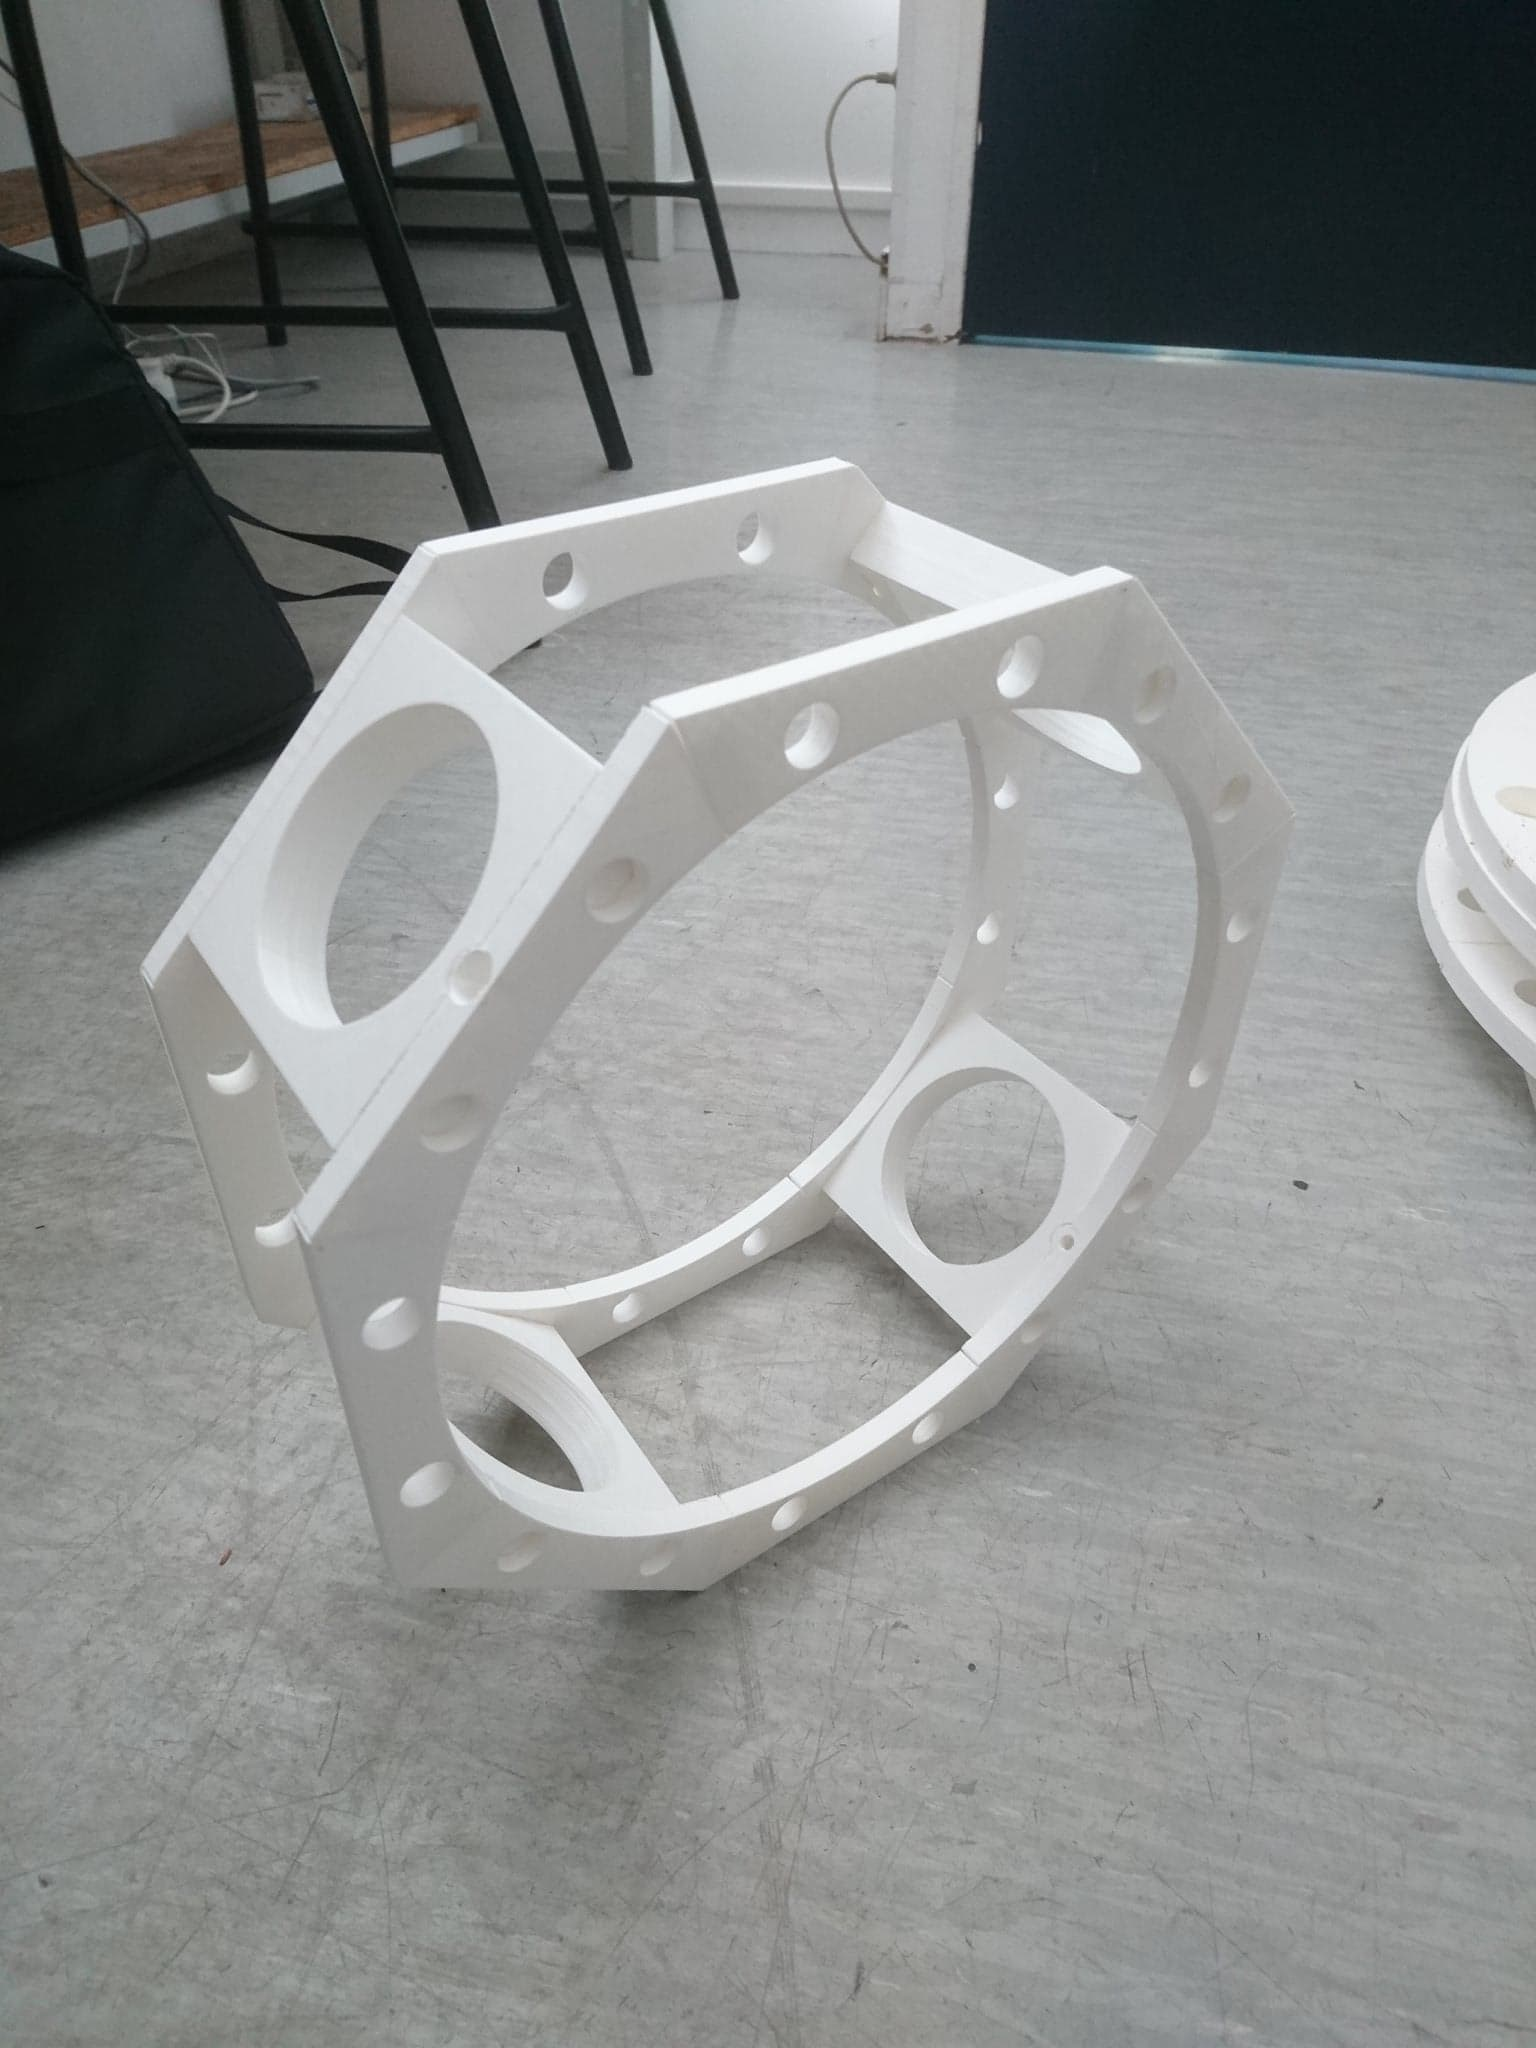
\includegraphics[width=0.3\linewidth]{\figures/photo_structure3.jpg}
    \decoRule
    \caption[
    Photos des parties montées du télescope]{
    Photos des parties montées du télescope}
    \label{fig:Photos des parties montées du télescope}
    \end{figure}


\chapter{Travail restant}

\section{Hardware}

Il reste pour cette partie la fabrication et la validation de la carte, ainsi que le câblage sur le télescope. Ces taches à défaut d'être difficiles sont assez chronophages.

\section{Système d'exploitation}

Le plus urgent est sans doute de réparer la configuration du Hotspot Wifi ainsi que de mettre en place une solution fiable pour transférer le flux vidéo de la caméra.

Ensuite, l'intégration des drivers et du logiciel principal pourront demander quelques configurations au niveau du kernel et du device tree.

Enfin, d'autres taches moins urgentes sont à réaliser, la mise en place d'un pare-feu et la sécurisation du système, la mise en place d'un système de mise à jour, sans doute \codeinline{text}{Mender} ou \codeinline{text}{SWupdate}. Puis diverses optimisations du système d'exploitation, retirer des choses inutiles, comme le daemon gérant le Bluetooth.

\section{Software}

Des travaux de réflexion sur les algorithmes à mettre en place pour mouvoir le télescope et calibrer ses actionneurs ont étés réalisés. Ceux-ci seront à approfondir conjointement aux autres membres du groupe pour écrire le logiciel principal du télescope dont des briques de base apparaissent par différentes extrémités.

\chapter{Organisation}

\section{Planning et répartition du travail}

En raison de l'abandon du projet par Thibaud LE DOLEDEC et Clément AILLOUD partis en stage, le projet ne pourra être mené à terme. Pour aborder la dernière ligne droite avant l'évaluation finale, un choix a donc été fait des tâches sur lesquelles travailler en priorité, au détriment d'autres qui demeureront inachevées.

\vspace{1cm}

Ci-dessous un diagramme représentant l’avancement des différentes tâches du projet. Le gris indique qu’une tâche est terminée ou à un niveau d’avancement satisfaisant et garantissant une maturité proche. Le orange indique les tâches en cours ou prioritaires au moment de l'évaluation finale. Les flèches représentent des liens de dépendance entre certaines tâches.

\begin{figure}[H]
    \centering
	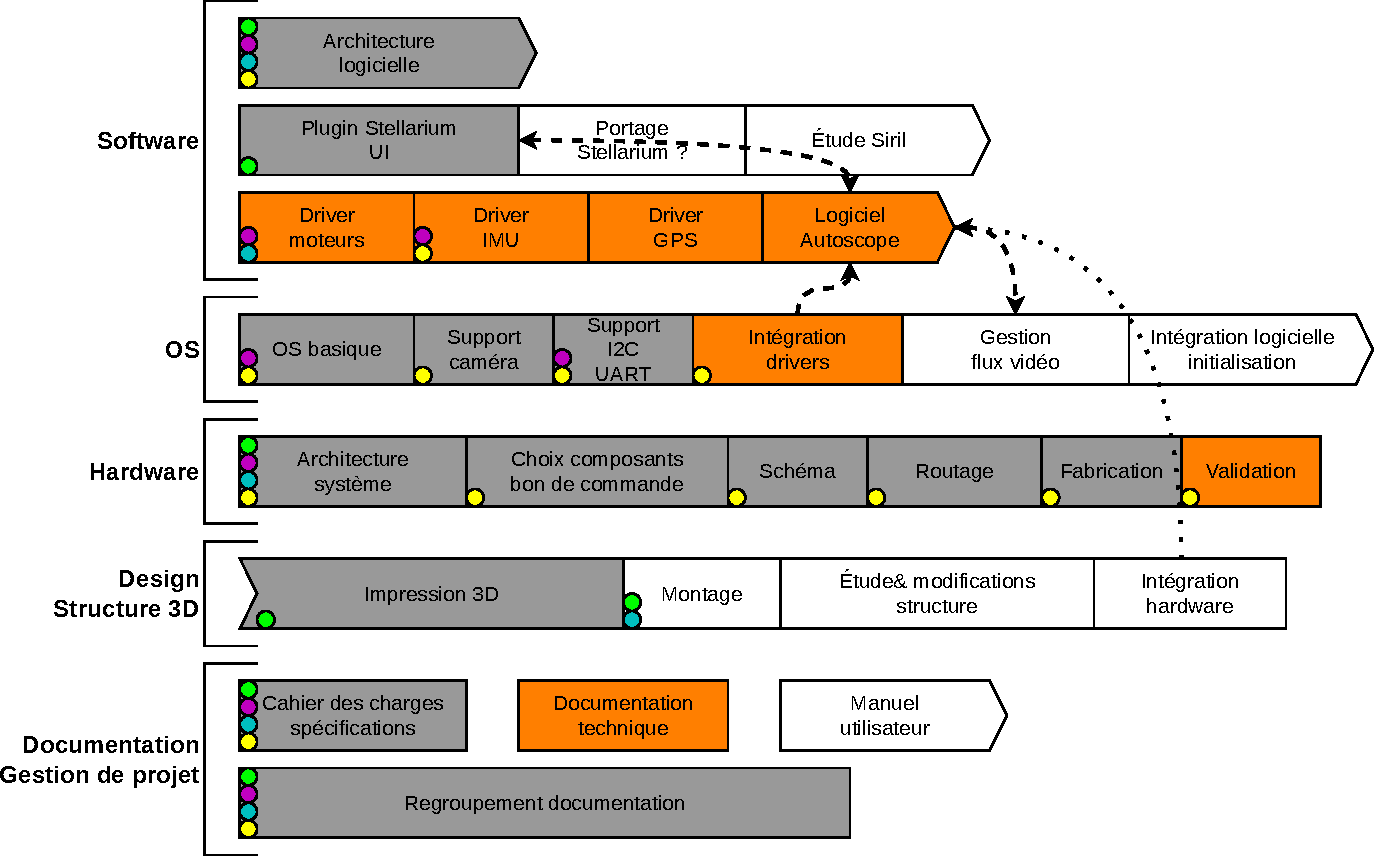
\includegraphics[width=1\linewidth]{\figures/sch_gantt.pdf}
    \decoRule
    \caption[
    Diagramme de l'organisation temporelle du travail sur le projet]{
    Diagramme de l'organisation temporelle du travail sur le projet}
    \label{fig:Diagramme de l'organisation temporelle du travail sur le projet}
    \end{figure}


\section{Accessibilité du projet sur internet}

Le projet étant libre, il est disponible sur Github sous licence GPL-2. Nous tachons d'accompagner nos différents dépôts d'une documentation claire permettant d'obtenir les informations suivantes~:
\begin{itemize}[label=$\bullet$]
	\item Une description brève et précise sur le contenu du dépôt et son rôle au sein du projet.
	\item Une explication de la procédure à suivre pour utiliser le contenu du dépôt.
	\item Une explication de la procédure à suivre pour travailler sur le dépôt.
	\end{itemize}

\subsection{Dépôt principal}

\url{https://github.com/thibaudledo/Autoscope}

\vspace{1cm}

Le dépôt est organisé comme suit~:
\begin{itemize}[label=$\bullet$]
	\item Branche {\href{https://github.com/thibaudledo/Autoscope/tree/master}{\codeinline{text}{master}}}~: Sources du logiciel principal et explications sur le projet dans son ensemble.
	\item Release {\href{https://github.com/thibaudledo/Autoscope/releases}{\codeinline{text}{alpha}}}~: Paquets et fichiers binaires pour utiliser le projet "out of the box" (release expérimentale).
	\item Branche {\href{https://github.com/thibaudledo/Autoscope/tree/hardware}{\codeinline{text}{hardware}}}~: Fichiers Blender de la structure du télescope et fichiers KiCad de la carte électronique du projet.
	\item Branche {\href{https://github.com/thibaudledo/Autoscope/tree/doc}{\codeinline{text}{doc}}}~: Documentations et datasheets des composants et éléments utilisés pour le projet.
	\item Branche {\href{https://github.com/thibaudledo/Autoscope/tree/latex}{\codeinline{text}{latex}}}~: Fichiers LaTex et \codeinline{text}{.pdf} des comptes rendus sur le projet.
	\item Branche {\href{https://github.com/thibaudledo/Autoscope/tree/hello_mod}{\codeinline{text}{hello_mod}}}~: Sources d'un driver helloworld servant d'exemple.
	\item Branche {\href{https://github.com/thibaudledo/Autoscope/tree/a4988_mod}{\codeinline{text}{a4988_mod}}}~: Sources du driver des contrôleurs moteur et des capteurs de fin de course des moteurs.
	\item Branche {\href{https://github.com/thibaudledo/Autoscope/tree/mpu9250_mod}{\codeinline{text}{mpu9250_mod}}}~: Sources du driver de la centrale inertielle.
	\item Branche {\href{https://github.com/thibaudledo/Autoscope/tree/mtk3339d}{\codeinline{text}{mtk3339d}}}~: Sources du driver du GPS.
	\end{itemize}

\newpage
\subsection{Dépôt du système d'exploitation de la Raspberry-Pi}

\url{https://github.com/thomaslepoix/meta-autoscope}

\vspace{1cm}

Il s'agit de la couche de métadonnées utilisées par Yocto pour construire le système d'exploitation Linux utilisé par la Raspberry-Pi du télescope. Une image pré-compilée du système d'exploitation figurera sur {\href{https://github.com/thibaudledo/Autoscope/releases}{la release \codeinline{text}{alpha} du dépôt principal}.

\vspace{1cm}

Le dépôt est organisé comme suit~:
\begin{itemize}[label=$\bullet$]
	\item Branche {\href{https://github.com/thomaslepoix/meta-autoscope/tree/rpi}{\codeinline{text}{rpi}}}~: Métadonnées Yocto et explications de comment compiler et installer le système d'exploitation.
	\item Branche {\href{https://github.com/thomaslepoix/meta-autoscope/tree/rpi-repo}{\codeinline{text}{rpi-repo}}}~: Données utilisées par Repo pour synchroniser le dépôt à d'autres dépôts de métadonnées Yocto utilisées pout construire l'OS.
	\end{itemize}

\subsection{Dépôt du plugin de Stellarium}

\url{https://github.com/thibaudledo/Autoscope-Stellarium-plugin}

\vspace{1cm}

Il s'agit du plugin de Stellarium contenant l'interface par laquelle l'utilisateur interagira avec le télescope. Un paquet pré-compilé pour linux de Stellarium incluant le plugin figure sur {\href{https://github.com/thibaudledo/Autoscope/releases}{la release \codeinline{text}{alpha} du dépôt principal}.

\vspace{1cm}

Le dépôt est organisé comme suit~:
\begin{itemize}[label=$\bullet$]
	\item Branche {\href{https://github.com/thibaudledo/Autoscope-Stellarium-plugin/tree/master}{\codeinline{text}{master}}}~: Sources du plugin, patch des sources de Stellarium et explications de comment compiler une version de Stellarium intégrant le plugin.
	\end{itemize}


\chapter{Travail effectué par Thibaud LE DOLEDEC et Clément AILLOUD}

\section{Driver de la centrale inertielle (IMU)}

Clément AILLOUD a développé un driver Linux pour la centrale inertielle en utilisant le framework \codeinline{text}{iio}. Celui-ci supporte actuellement le gyroscope et l'accéléromètre mais pas le magnétomètre. Il est compatible avec les bus I2C et SPI. Sur l'Autoscope, le bus I2C sera utilisé.

Un patch du device tree permettant le support du driver est également fourni.

\vspace{1cm}

Le driver a été intégré au système d'exploitation du télescope. \codeinline{text}{iio} permet d'accéder aux données issues de l'IMU via le dossier suivant~:

\code{text}
root@autoscope ~ #
    ls /sys/bus/iio/devices/iio:device0/
        dev               in_accel_y_raw    in_anglvel_x_raw  in_temp_input  power
        in_accel_scale    in_accel_z_raw    in_anglvel_y_raw  name           subsystem
        in_accel_x_raw    in_anglvel_scale  in_anglvel_z_raw  of_node        uevent

    cat /sys/bus/iio/devices/iio:device0/name
        mpu9250-i2c
\end{minted}

\section{Interface utilisateur (Plugin de Stellarium)}

Le logiciel Stellarium offre la possibilité de développer des plugins aux fonctionnalités diverses. Nous avons décidé d'utiliser un plugin pour faire de Stellarium l'élément principal de l'interface utilisateur du télescope.

\vspace{1cm}

Thibaud LE DOLEDEC a développé un plugin de Stellarium permettant les actions suivantes~:
\begin{itemize}[label=$\bullet$]
	\item Rechercher un astre et le suivre tant à l'écran qu'avec le télescope (par l'envoi régulier de coordonnées spatiales à celui-ci).
	\item Demander au télescope ses coordonnées de position et de visée et afficher la vue du ciel simulé correspondante.
	\item Ordonner au télescope de prendre une photo. Il existe une interface destinée à configurer les paramètres de la caméra (temps d'exposition, etc.).
	\item Se connecter au serveur FTP du télescope pour récupérer les clichés du ciel.
	\item Afficher un aperçu de ce que voit le télescope à l'instant présent (retransmission d'un flux vidéo). Un espace actuellement matérialisé par un rectangle gris est destiné à cela.
	\end{itemize}

\vspace{1cm}

\begin{figure}[H]
    \centering
    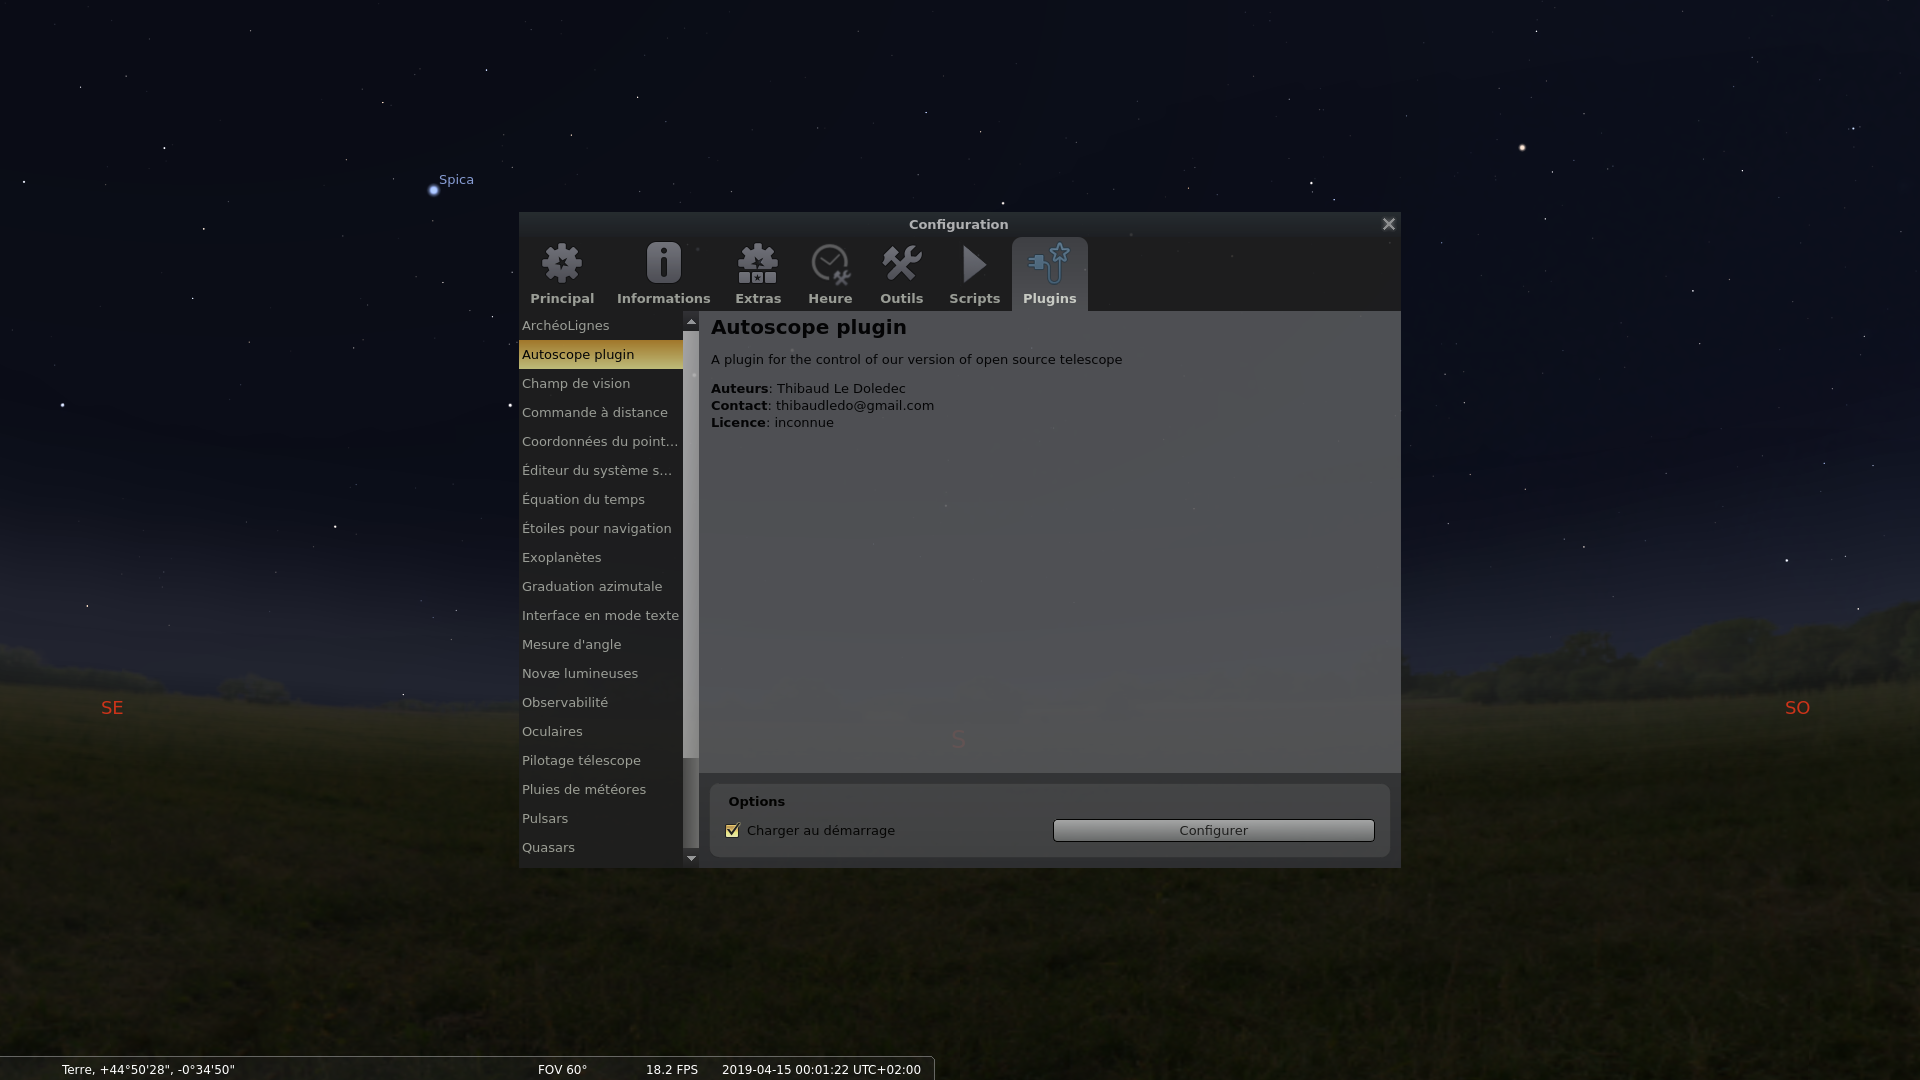
\includegraphics[width=0.9\linewidth]{\figures/photo_stellarium_3.png}
    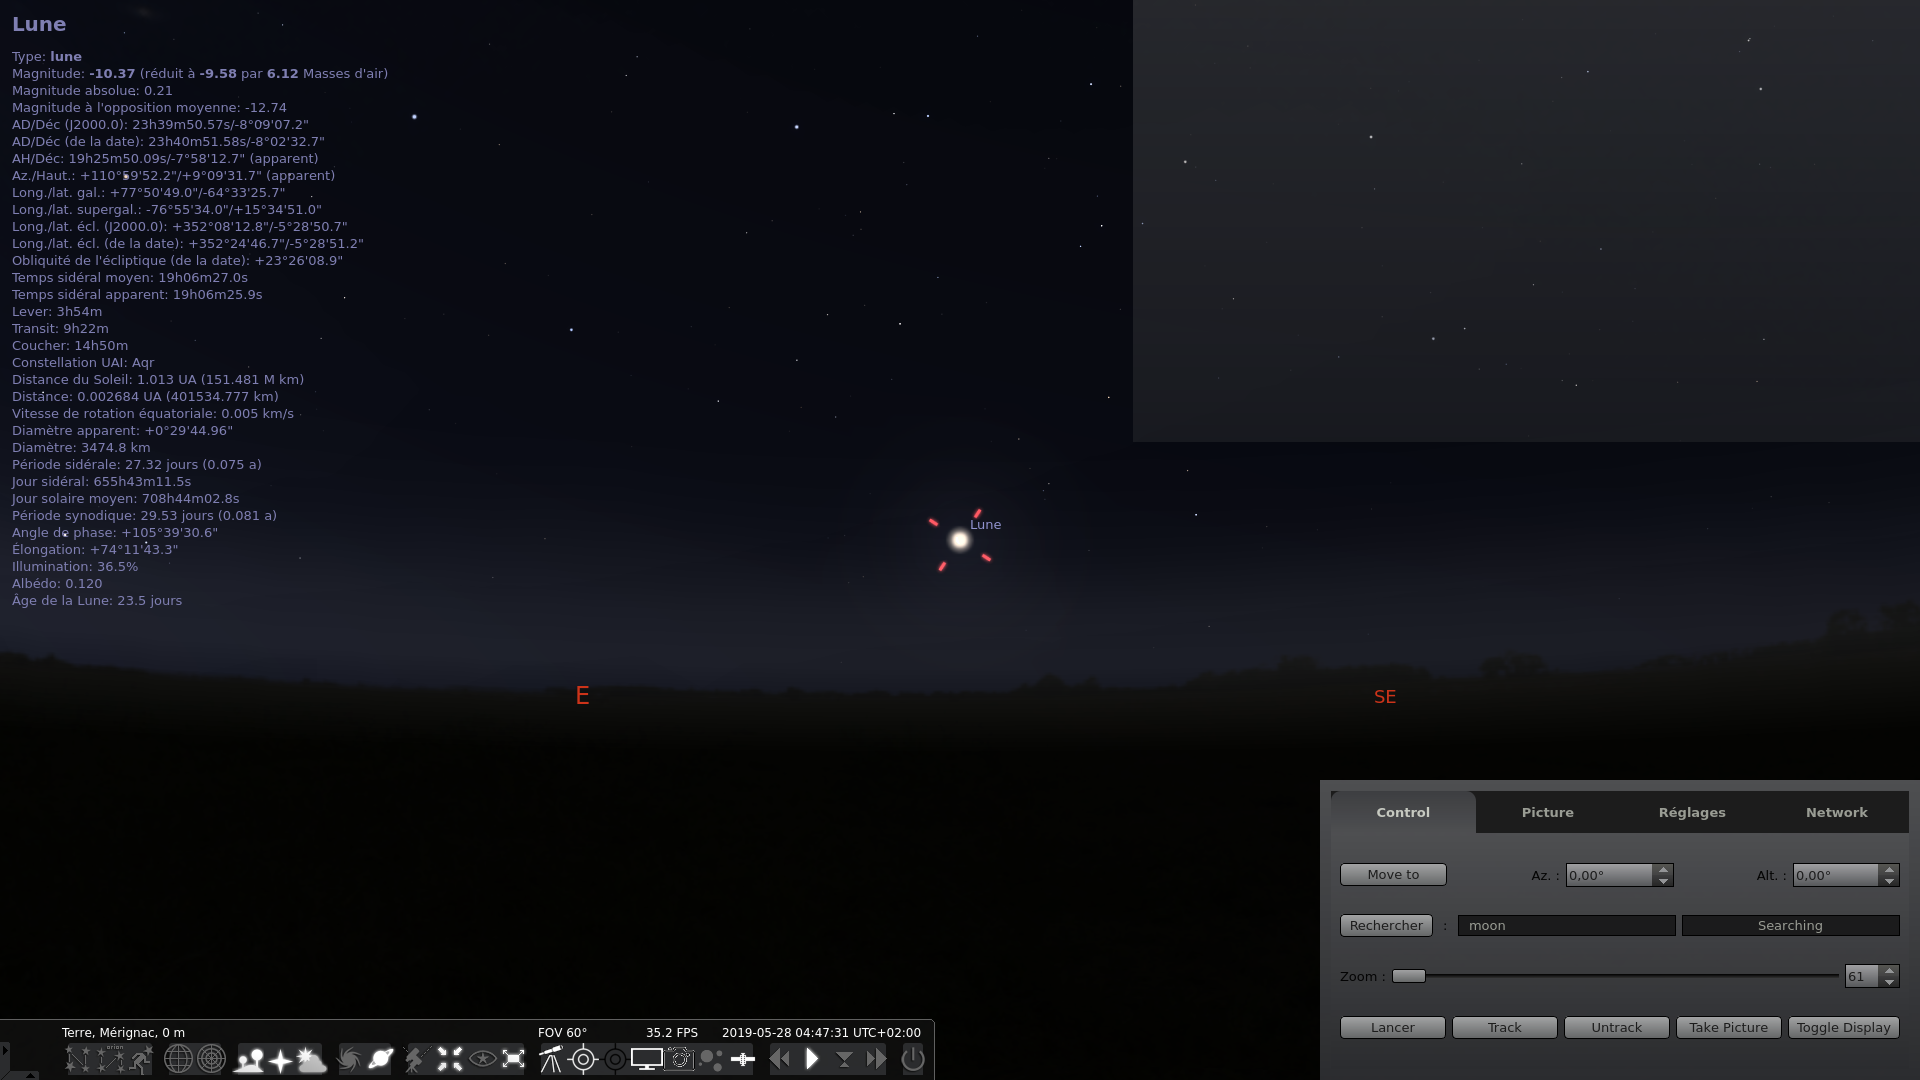
\includegraphics[width=0.9\linewidth]{\figures/photo_stellarium_4.png}
    \decoRule
    \caption[
    Aperçu de l'interface du plugin de Stellarium]{
    Aperçu de l'interface du plugin de Stellarium}
    \label{fig:Aperçu de l'interface du plugin de Stellarium}
    \end{figure}

\vspace{1cm}

Le plugin fonctionne correctement, bien que certains éléments soient sûrement à retravailler lors du développement du logiciel principal du télescope.

La gestion de la communication FTP repose sur l'utilisation d'une librairie dépréciée \codeinline{text}{qtftp} qui a semblé poser problème lors des essais de déploiement du travail réalisé par Thibaud. L'idéal serait de se passer de cette librairie.

\vspace{1cm}

Thibaud et Clément ont rédigé un document disponible à l'adresse suivante qui explique la procédure à suivre pour développer un plugin de Stellarium.

{\href{https://github.com/thibaudledo/Autoscope/blob/latex/Tutoriel_Stellarium.pdf}{\codeinline{text}{https://github.com/thibaudledo/Autoscope/blob/latex/Tutoriel_Stellarium.pdf}}}

\chapter{Travail restant à faire}

Ce chapitre existe dans le but de récapituler le travail restant à faire sur le projet de façon un minimum exhaustive.

\section{Structure du télescope}

La plupart des pièces du télescope vierge de toute modification a été imprimée, quelques parties assemblées. Le travail restant à faire est conséquent et consiste en la modification du design du télescope en vue d'y intégrer~:
\begin{itemize}[label=$\bullet$]
	\item La carte électronique et la Raspberry-pi, face vers le sol, sous le miroir primaire.
	\item Les modules GPS et IMU, placés le long de la structure du télescope. L'interprétation des données émises par l'IMU dépendra de son positionnement.
	\item Les moteurs d'azimut et d'élévation ainsi que leurs courroies et tringles. Les roues crantées à fixer sur l'axe des moteurs n'ont pas été choisies. Leur diamètre reste à déterminer.
	\item Les boutons poussoirs, capteurs de fin de course des mouvements engendrés par les moteur. Leur position devra être déterminée avec précision.
	\item Tout le dispositif maintenant l'oculaire, le moteur permettant de l'actionner, les capteurs de fin de course associés (le mouvement de l'oculaire s'étend sur environ un quart de tour), ainsi que le module caméra. Ce dispositif devra être conçu avec le plus grand soin et la plus grande attention afin de permettre un réglage fin du télescope et d'obtenir une image nette. Il est conseillé de se renseigner la procédure de $collimation$ des télescopes avant de se lancer dans la conception.
	\end{itemize}

\section{Hardware}

Il reste uniquement à faire la connectique des éléments déportés de la carte électronique.

Un ventilateur de refroidissement du miroir peut aussi être choisi, nous ne nous sommes pas renseignés sur l'utilité avérée ou non de cet élément.

\section{Système d'exploitation}

\begin{itemize}[label=$\bullet$]
	\item Sécurisation du système par la mise en place d'un pare feu avec \codeinline{text}{iptables} (et donc l'étude des ports utilisés, ainsi que le choix d'un port ne posant aucun conflit pour le transfert vidéo et la communication avec le plugin Stellarium), une gestion plus fine des droits de chaque utilisateur Linux, etc. L'abandon de FTP au profit de SFTP comme protocole de transfert d'images serait souhaitable (\codeinline{text}{openSSH} déjà utilisé comme serveur SSH permet cela).
	\item La mise en place d'un système de mise à jour de l'OS. \codeinline{text}{SWUpdate} semble être une solution plus intéressante que \codeinline{text}{Mender} puisque nettement plus souple et configurable, tant dans la façon de mettre à jour le système que dans la façon de déclencher la mise à jour. Dans tous les cas, ces systèmes de mise à jour nécessitent d'utiliser un bootloader en plus du firmware du GPU de la Raspberry-Pi, or l'overlay du device tree \codeinline{text}{pi3-disable-bt} (nécessaire pour la communication avec le GPS) semble être incompatible avec U-Boot. Une tentative de transformer l'overlay en patch n'a pas résolu le problème, les investigations n'ont pas été poussées davantage.
	\item L'optimisation de l'OS. Plusieurs choses peuvent être optimisées, la mémoire occupée, le temps de boot (qui peut être optimisé à plusieurs niveau, les plus faciles à travailler étant le niveau applicatif et le niveau de processus d'initialisation, ensuite viennent Linux et bootloader). Sur Yocto, le fichier \codeinline{text}{meta-autoscope/conf/distro/autoscope.conf} permet de se délester du support d'éléments inutilisés. Le lien suivant est une documentation intéressante~:\\\url{https://embexus.com/2017/05/16/embedded-linux-fast-boot-techniques/}
	\end{itemize}

\section{Support de la caméra}

Il faut évaluer les possibilités de paramétrage de la capture photo que permettent les logiciels \codeinline{text}{raspistill}, \codeinline{text}{raspiyuv}, etc. Peut être cela est suffisant, peut être existe il une librairie de plus bas niveau utilisable dans un programme C/C++, peut être sera il nécessaire d'en développer une. Il semble peu probable qu'il faille modifier le driver de la caméra.

\section{Transfert du flux vidéo sur le réseau}

La communauté Raspberry-Pi fournit une librairie Python de contrôle de la caméra, il semble qu'elle permette un transfert sur le réseau du flux vidéo sans latence excessive. La recette Yocto pour intégrer ladite librairie a été écrite mais pas celle permettant l'ajout de toutes celles qu'elle même utilise.

Il serait préférable de trouver une librairie équivalente en C/C++, ou à défaut de l'écrire.

\vspace{1cm}

Il n'a pas été déterminé s'il est plus pertinent d'intégrer le logiciel de transmission du flux vidéo au logiciel principal du télescope ou s'il est plus pertinent d'en faire un autre logiciel.

Le serveur vidéo devra probablement s'interrompre le temps que le télescope utilise la caméra pour prendre une photo ponctuelle. Dans le cas où il serait un logiciel distinct du logiciel principal, les signaux seraient sûrement pour ce dernier un moyen de contrôle suffisant. Par exemple \codeinline{text}{SIGSTOP} et \codeinline{text}{SIGCONT} s'il suffit de mettre le serveur en pause, \codeinline{text}{SIGUSR1} et \codeinline{text}{SIGUSR2} si le serveur doit effectuer des actions de connexion/déconnexion au client ainsi qu'à la caméra.

\section{Daemon du GPS}

Le daemon du GPS n'a pas été testé dans un environnement où la connexion est suffisamment bonne pour que le GPS parvienne à calculer sa position géographique. Il suffit probablement de l'emmener à l'extérieur. Ce test permettrait de valider définitivement le fonctionnement du daemon ainsi que du GPS.

%TODO
\section{Driver des contrôleurs moteur}
%TODO
\section{Driver de la centrale inertielle (IMU)}
\section{Plugin de Stellarium}

\begin{itemize}[label=$\bullet$]
	\item La librairie FTP utilisée \codeinline{text}{qftp} pose problème et est dépréciée, il faudrait se passer de son utilisation. Il serait judicieux d'en profiter pour migrer vers SFTP, plus sécurisé.
	\item Une partie du code sera probablement à retravailler conjointement au développement du logiciel principal du télescope, ainsi que du serveur vidéo.
	\end{itemize}

\section{Logiciel principal du télescope (Autoscope-core)}

\begin{itemize}[label=$\bullet$]
	\item Intégration dans un programme unique des fragments d'interface avec les différents organes logiciels du télescope (drivers moteurs et IMU, daemon GPS, plugin Stellarium, etc). Ces fragments se trouvent sur la branche {\href{https://github.com/thibaudledo/Autoscope/tree/master}{\codeinline{text}{master} du dépôt git principal}} et sont voués à disparaître une fois cette tâche effectuée.
	\item Développement de l'algorithme de déplacement du télescope. Celui-ci va dépendre des données qu'il est possible d'obtenir de la centrale inertielle, des possibilités du driver des contrôleurs moteur, ainsi que de la structure du télescope et la façon dont sera intégrée le hardware.
	\end{itemize}


\part{Thomas LEPOIX}
%\chapter{Avancement général}

En raison de l'abandon du projet par Thibaud LE DOLEDEC et Clément AILLOUD partis en stage, le projet ne pourra être mené à terme. Pour aborder la dernière ligne droite avant l'évaluation finale, un choix a donc été fait des taches sur lesquelles travailler en priorité, au détriment d'autres qui demeureront inachevées.

\vspace{1cm}

Ci-dessous un diagramme représentant l’avancement des différentes taches du projet. Le gris indique qu’une tache est terminée ou à un niveau d’avancement satisfaisant et garantissant une maturité proche. Le orange indique les taches sur lesquelles nous travaillerons en priorité avant la fin du projet. Les flèches représentent des liens de dépendance entre les taches.

\begin{figure}[H]
    \centering
	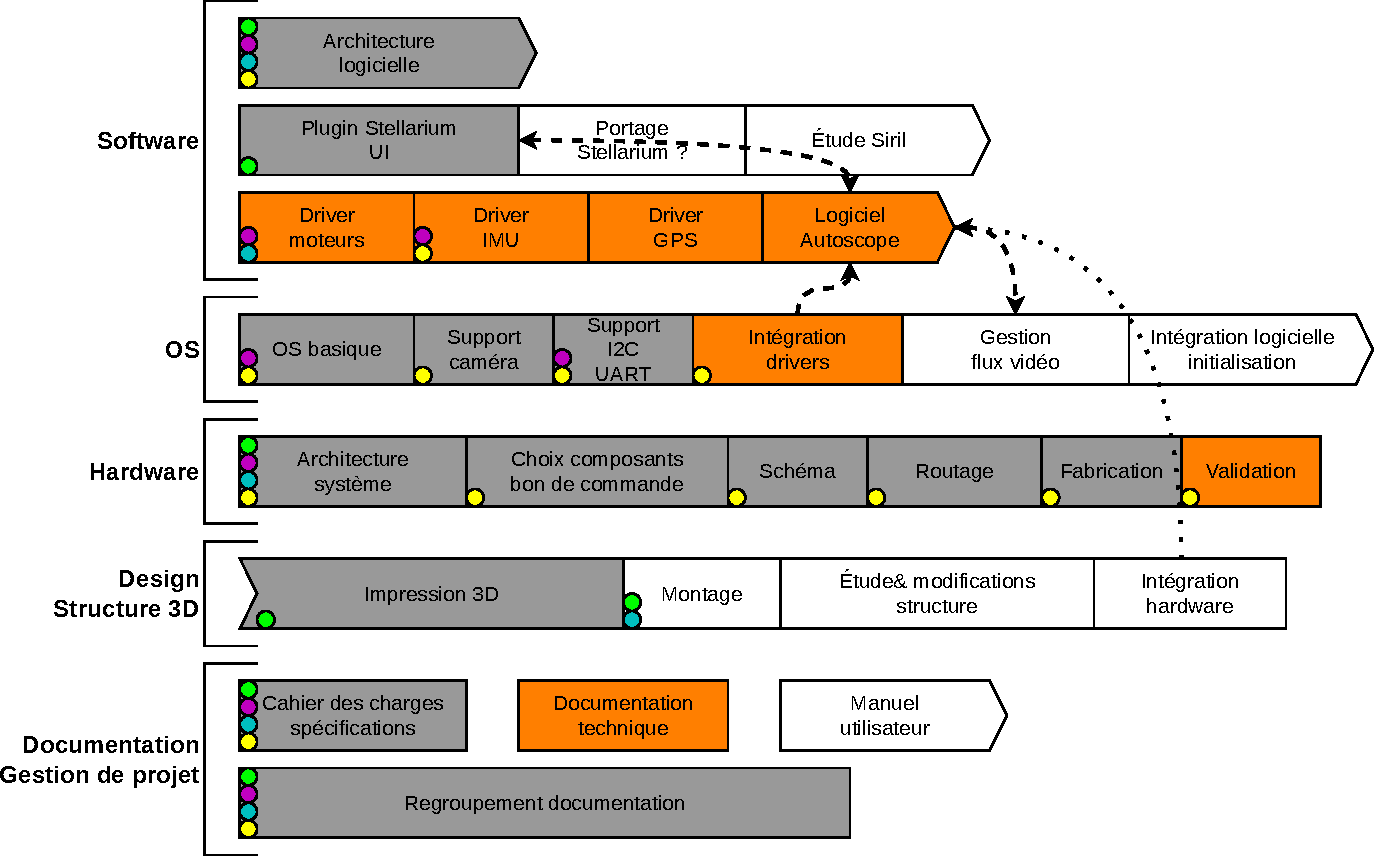
\includegraphics[width=1\linewidth]{\figures/sch_gantt.pdf}
    \decoRule
    \caption[
    Diagramme de l'organisation temporelle du travail sur le projet]{
    Diagramme de l'organisation temporelle du travail sur le projet}
    \label{fig:Diagramme de l'organisation temporelle du travail sur le projet}
    \end{figure}

\section{Prévisions pour le dernier sprint}

Malgré son aspect visuel intéressant pour promouvoir le projet ainsi que de sont aspect central (il s'agit tout de même d'un télescope), le travail sur la structure du télescope sera écarté des taches prioritaires. Cela pour deux raisons~:
\begin{itemize}[label=$\bullet$]
	\item Il s'agit d'une partie du projet demandant beaucoup de temps et d'implications par rapport à ce dont nous disposons. Nous n'aurions sans doute pas le temps de terminer cela avant l'évaluation.
	\item N'ayant ni des connaissances particulières en optique, ni la maîtrise d'un logiciel de modélisation 3D, nous ne sommes pas plus qualifiés qu'une personne aléatoire voulant contribuer au projet. Nous pensons donc qu'il vaut mieux nous concentrer sur des taches faisant partie de notre domaine de qualification, que nous serions capable de réaliser plus facilement ou mieux qu'une personne aléatoire. L'élaboration des drivers correspond typiquement à ce cas.
	\end{itemize}

\vspace{1cm}

Le travail sur les drivers, quant à lui devra être avancé autant que faire se peut. En effet le logiciel principal du télescope dépend lourdement des interfaces avec les drivers et ne peut être commencé tant que les drivers ne sont pas fonctionnels.

De plus, ce logiciel étant la clef de voûte du projet, la finalisation de certaines taches comme certains éléments du plugin Stellarium ou la gestion du flux vidéo au sein de l'OS doit être réalisée conjointement à l'écriture de ce logiciel.

L'absence des ces drivers commence donc à bloquer l'évolution d'autres taches.

\vspace{1cm}

Enfin un travail de documentation devra être fait pour qu'il soit possible à une personne future (nous-mêmes ou qui que ce soit) de travailler sur ce projet ou de réutiliser notre travail.





\chapter{Accessibilité au projet sur internet}

Le projet étant libre, il est disponible sur Github sous licence GPL-2. Nous tachons d'accompagner nos différents dépôts d'une documentation claire permettant d'obtenir les informations suivantes~:
\begin{itemize}[label=$\bullet$]
	\item Une description brève et précise sur le contenu du dépôt et son rôle au sein du projet.
	\item Une explication de la procédure à suivre pour utiliser le contenu du dépôt.
	\item Une explication de la procédure à suivre pour travailler sur le dépôt.
	\end{itemize}

\section{Dépôt principal}

\url{https://github.com/thibaudledo/Autoscope}

\vspace{1cm}

Le dépôt est organisé comme suit~:
\begin{itemize}[label=$\bullet$]
	\item Branche {\href{https://github.com/thibaudledo/Autoscope/tree/master}{\codeinline{text}{master}}}~: Licence du projet et explications sur le projet dans son ensemble.
	\item Release {\href{https://github.com/thibaudledo/Autoscope/releases}{\codeinline{text}{alpha}}}~: Paquets et fichiers binaires pour utiliser le projet "out of the box" (release expérimentale).
	\item Branche {\href{https://github.com/thibaudledo/Autoscope/tree/hardware}{\codeinline{text}{hardware}}}~: Fichiers Blender de la structure du télescope et fichiers KiCad de la carte électronique du projet.
	\item Branche {\href{https://github.com/thibaudledo/Autoscope/tree/doc}{\codeinline{text}{doc}}}~: Documentations et datasheets des composants et éléments utilisés pour le projet.
	\item Branche {\href{https://github.com/thibaudledo/Autoscope/tree/latex}{\codeinline{text}{latex}}}~: Fichiers LaTex et \codeinline{text}{.pdf} des comptes rendus sur le projet.
	\item Branche {\href{https://github.com/thibaudledo/Autoscope/tree/hello_mod}{\codeinline{text}{hello_mod}}}~: Sources d'un driver helloworld servant d'exemple.
	\item Branche {\href{https://github.com/thibaudledo/Autoscope/tree/a4988_mod}{\codeinline{text}{a4988_mod}}}~: Sources du driver des contrôleurs moteur et des capteurs de fin de course des moteurs.
	\item Branche {\href{https://github.com/thibaudledo/Autoscope/tree/mpu_9250_mod}{\codeinline{text}{mpu_9250_mod}}}~: Sources du driver de la centrale inertielle.
	\item Branche {\href{https://github.com/thibaudledo/Autoscope/tree/mtk3339_mod}{\codeinline{text}{mtk3339_mod}}}~: Sources du driver du GPS.
	\end{itemize}

\newpage
\section{Dépôt du système d'exploitation de la Raspberry-Pi}

\url{https://github.com/thomaslepoix/meta-autoscope}

\vspace{1cm}

Il s'agit de la couche de métadonnées utilisées par Yocto pour construire le système d'exploitation Linux utilisé par la Raspberry-Pi du télescope. Une image pré-compilée du système d'exploitation figurera sur {\href{https://github.com/thibaudledo/Autoscope/releases}{la release \codeinline{text}{alpha} du dépôt principal}.

\vspace{1cm}

Le dépôt est organisé comme suit~:
\begin{itemize}[label=$\bullet$]
	\item Branche {\href{https://github.com/thomaslepoix/meta-autoscope/tree/rpi}{\codeinline{text}{rpi}}}~: Métadonnées Yocto et explications de comment compiler et installer le système d'exploitation.
	\item Branche {\href{https://github.com/thomaslepoix/meta-autoscope/tree/rpi-repo}{\codeinline{text}{rpi-repo}}}~: Données utilisées par Repo pour synchroniser le dépôt à d'autres dépôts de métadonnées Yocto utilisées pout construire l'OS.
	\end{itemize}

\section{Dépôt du plugin de Stellarium}

\url{https://github.com/thibaudledo/Autoscope-Stellarium-plugin}

\vspace{1cm}

Il s'agit du plugin de Stellarium contenant l'interface par laquelle l'utilisateur interagira avec le télescope. Un paquet pré-compilé pour linux de Stellarium incluant le plugin figure sur {\href{https://github.com/thibaudledo/Autoscope/releases}{la release \codeinline{text}{alpha} du dépôt principal}.

\vspace{1cm}

Le dépôt est organisé comme suit~:
\begin{itemize}[label=$\bullet$]
	\item Branche {\href{https://github.com/thibaudledo/Autoscope-Stellarium-plugin/tree/master}{\codeinline{text}{master}}}~: Sources du plugin, patch des sources de Stellarium et explications de comment compiler une version de Stellarium intégrant le plugin.
	\end{itemize}


\chapter{Structure du télescope}

\section{Projet d'origine}

La structure du télescope est imprimable à l'imprimante 3D et provient d'un projet open source entre temps disparu d'internet~:
\url{https://blog.dagoma.fr/telescope-imprime-en-3d/}

\vspace{1cm}

Voici l'allure du télescope monté. Les barres métalliques raccordant le support du miroir secondaire au reste du télescope sont des barres de camping achetées en magasin de sport.

\begin{figure}[H]
    \centering
    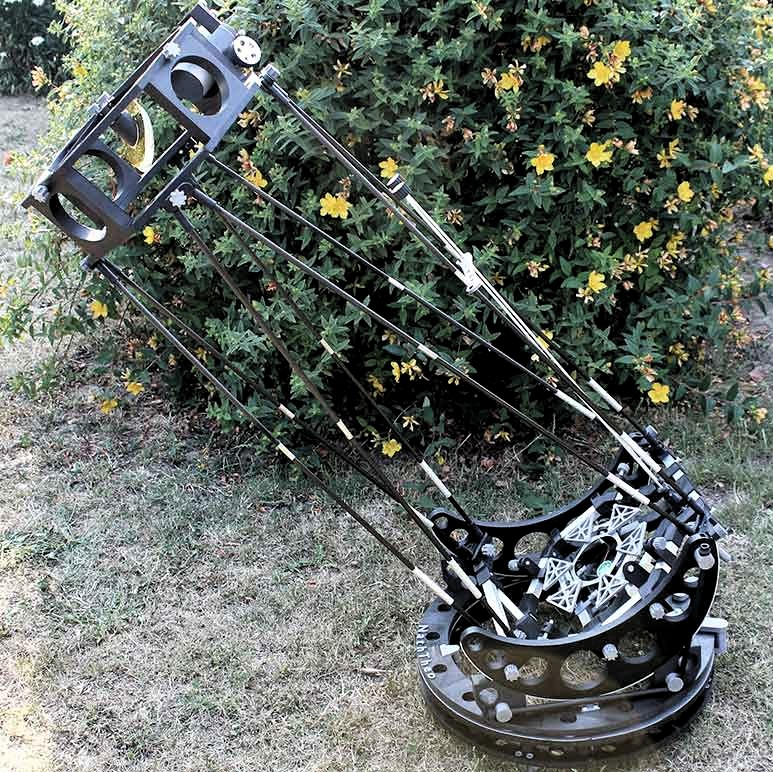
\includegraphics[width=0.5\linewidth]{\figures/photo_telescope2.jpg}
    \decoRule
    \caption[
    Photo du télescope]{
    Photo du télescope}
    \label{fig:Photo du télescope}
    \end{figure}

\begin{figure}[H]
    \centering
    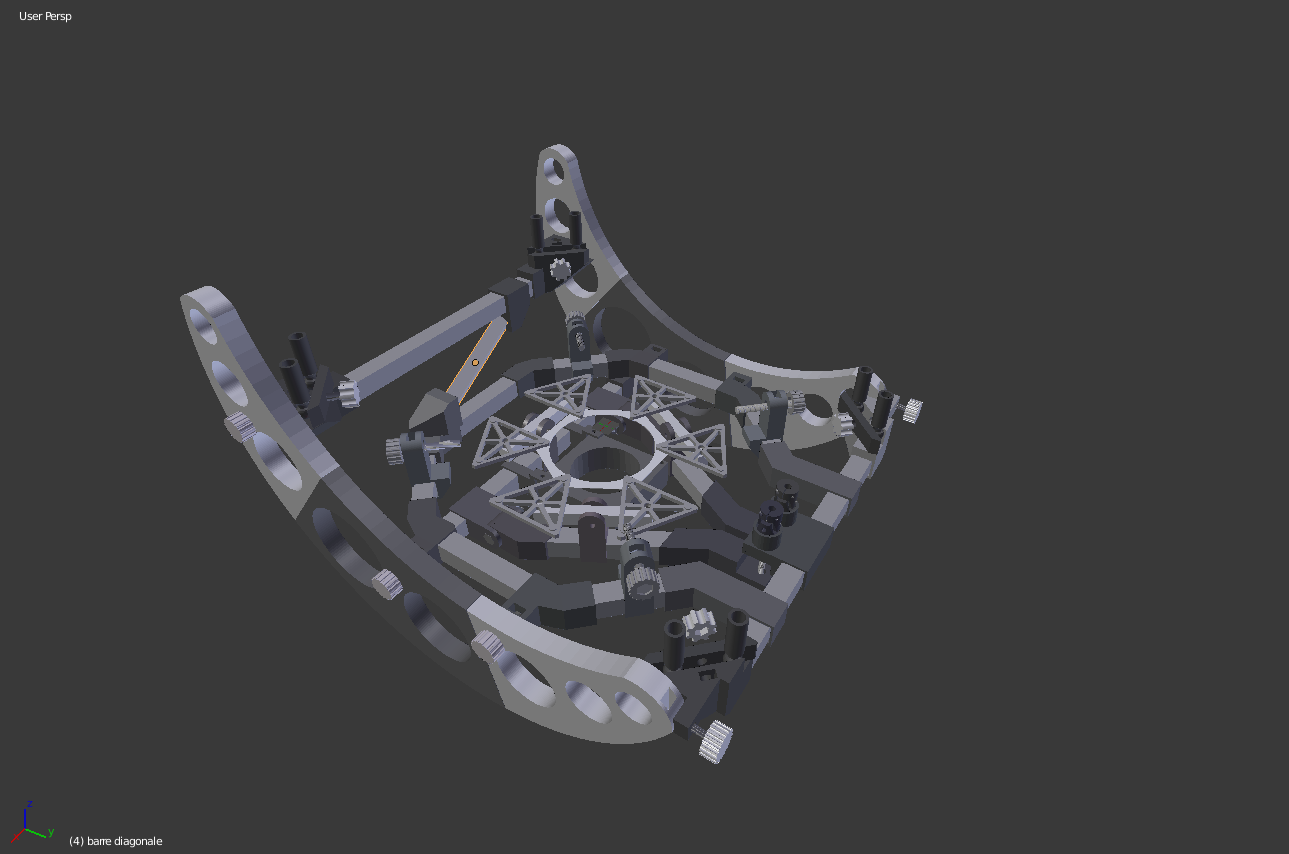
\includegraphics[width=0.49\linewidth]{\figures/blender_3.png}
    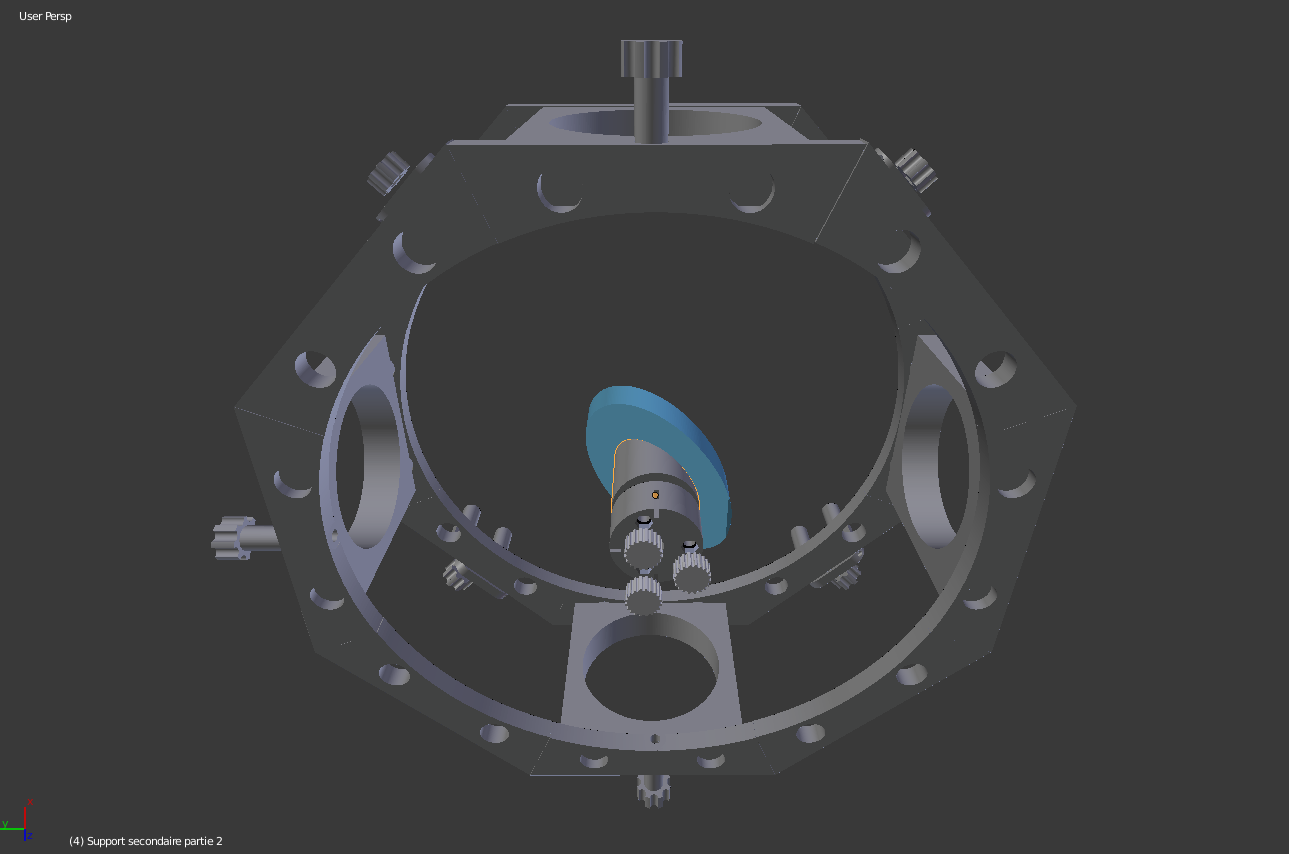
\includegraphics[width=0.49\linewidth]{\figures/blender_4.png}
    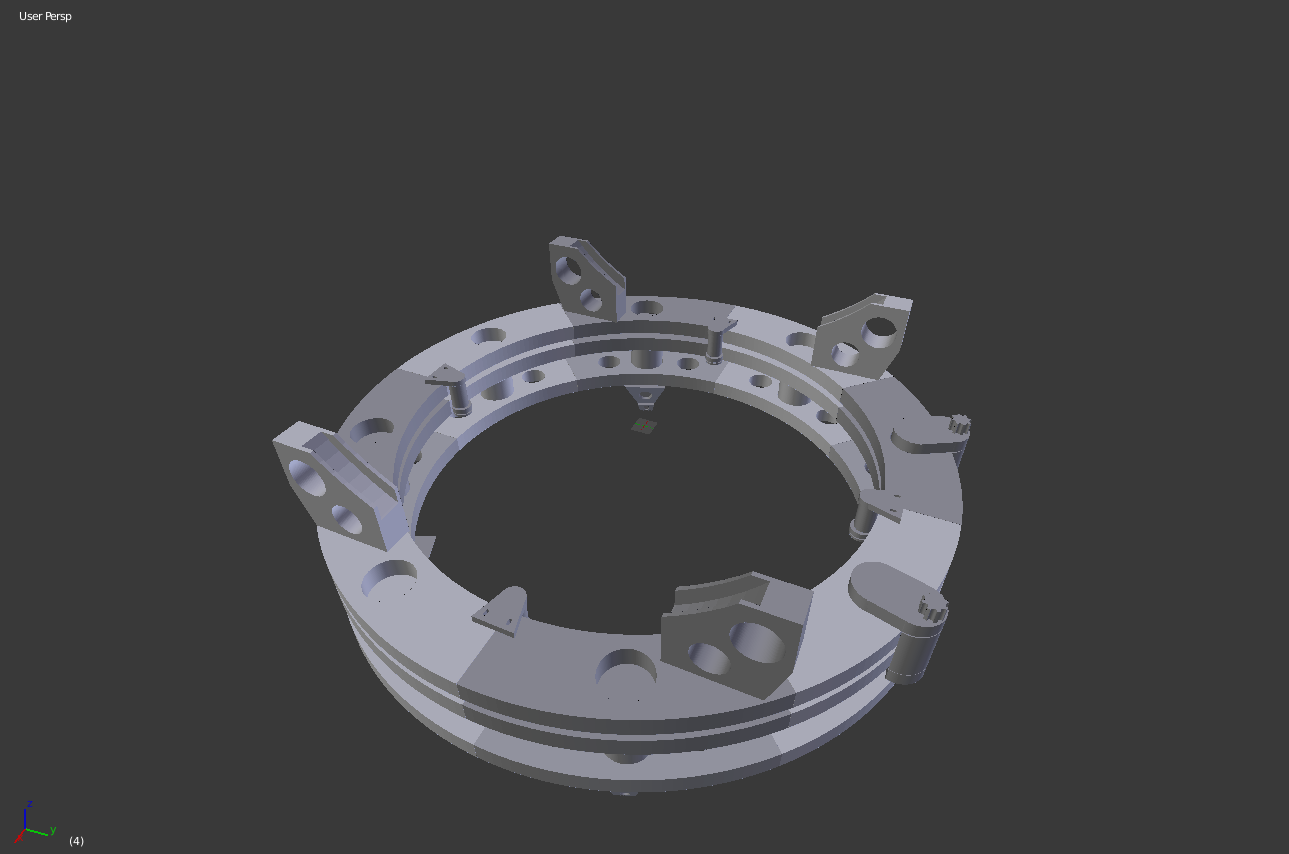
\includegraphics[width=0.49\linewidth]{\figures/blender_5.png}
    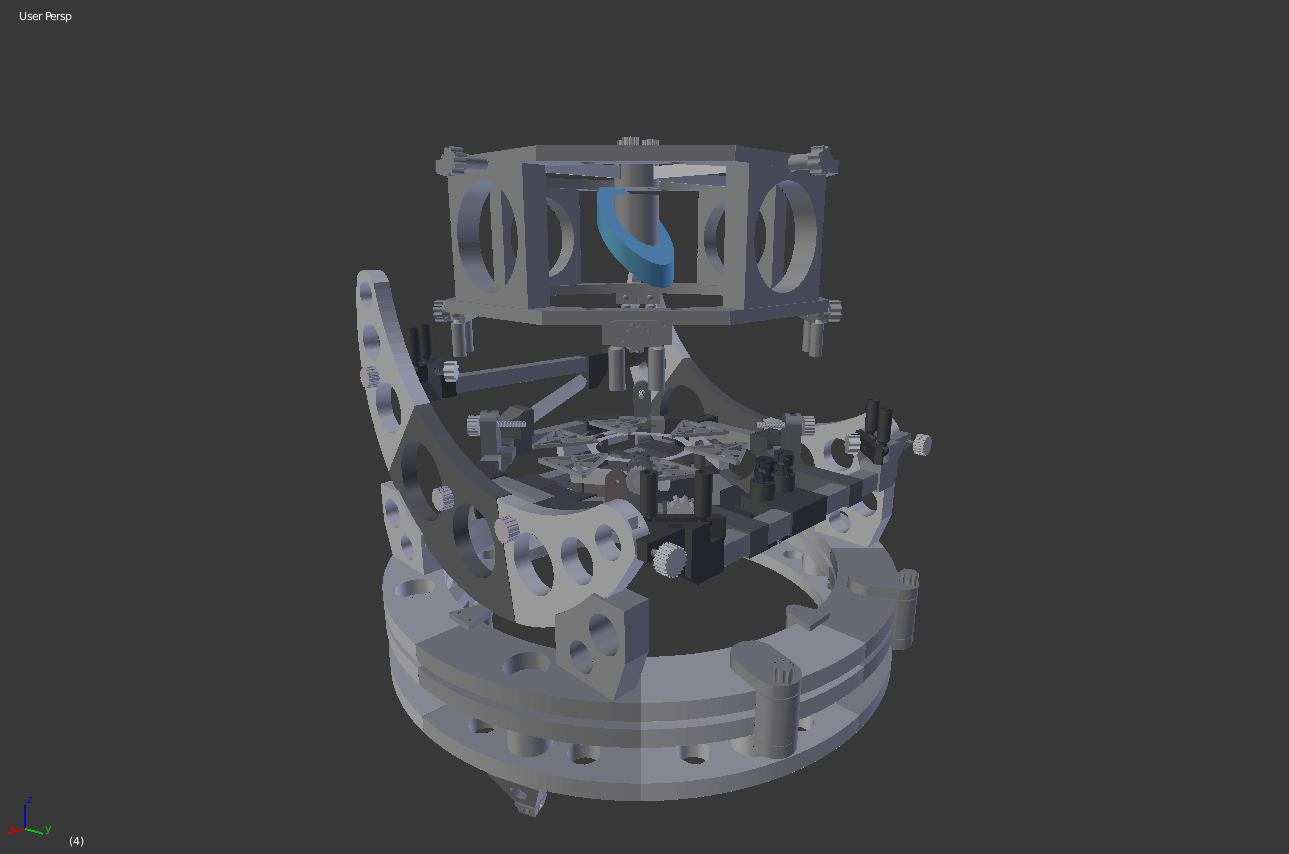
\includegraphics[width=0.49\linewidth]{\figures/blender_6.png}
    \decoRule
    \caption[
    Aperçu des fichiers de production du télescope]{
    Aperçu des fichiers de production du télescope}
    \label{fig:Aperçu des fichiers de production du télescope}
    \end{figure}

\section{Étude de la robotisation du télescope}

Ci-dessous quelques schémas représentant les modifications, telles qu'imaginées, à apporter à la structure du télescope pour l'automatiser.

\vspace{1cm}

Le socle, immobile, sera doté d'une courroie ainsi que d'un cran permettant d'activer le capteur de position. Le système électronique sera solidaire du support du miroir primaire, mobile, à l'étage supérieur. Un moteur doté d'une roue crantée fixé sur la plateforme tournante permettra de la mettre en mouvement par rapport au socle.

\begin{figure}[H]
    \centering
    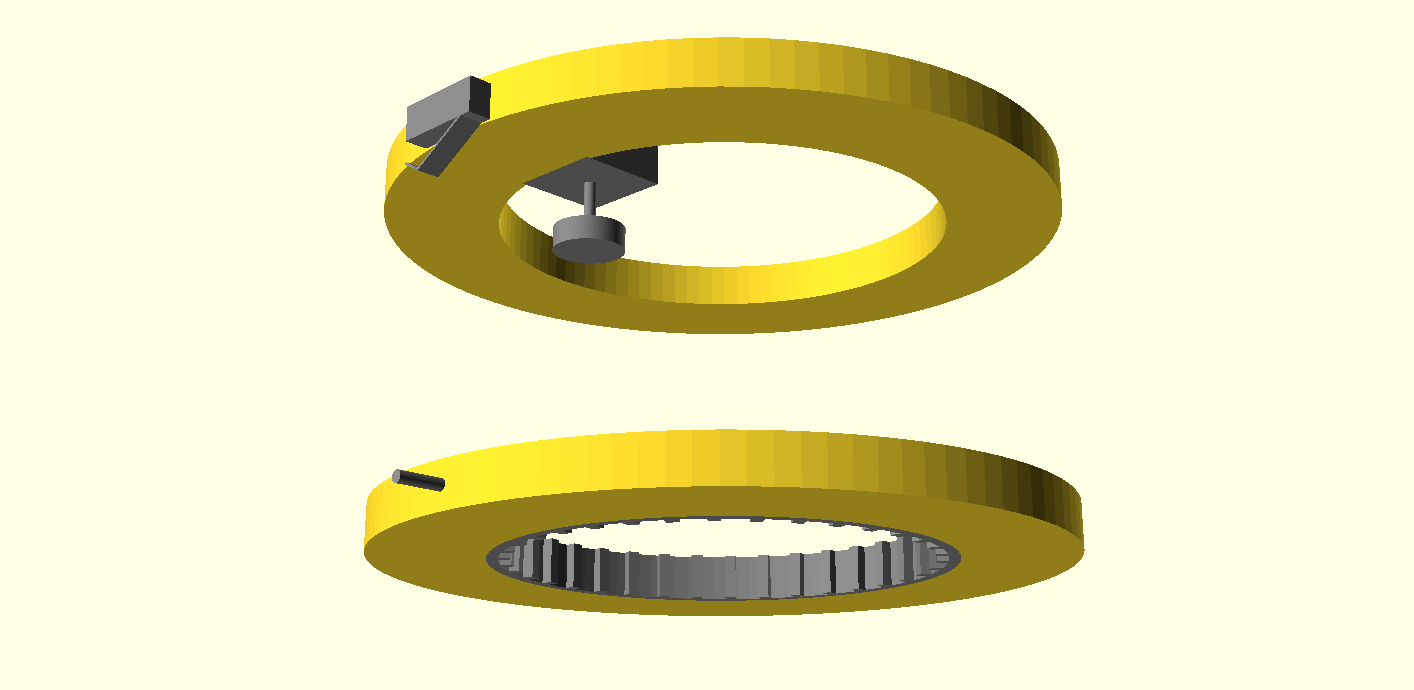
\includegraphics[width=0.9\linewidth]{\figures/OpenSCAD/azim.png}
    \decoRule
    \caption[
    Schéma du mécanisme permettant un mouvement azimutal]{
    Schéma du mécanisme permettant un mouvement azimutal}
    \label{fig:Schéma du mécanisme permettant un mouvement azimutal}
    \end{figure}

\vspace{1cm}

Pour le mouvement d'élévation, un système de tringlerie et de courroie a été imaginé pour mouvoir le support du miroir primaire par rapport à la plateforme tournante. Deux capteurs de position judicieusement placés permettront de détecter lorsque le mouvement atteint l'un de ses maximums.

\begin{figure}[H]
    \centering
    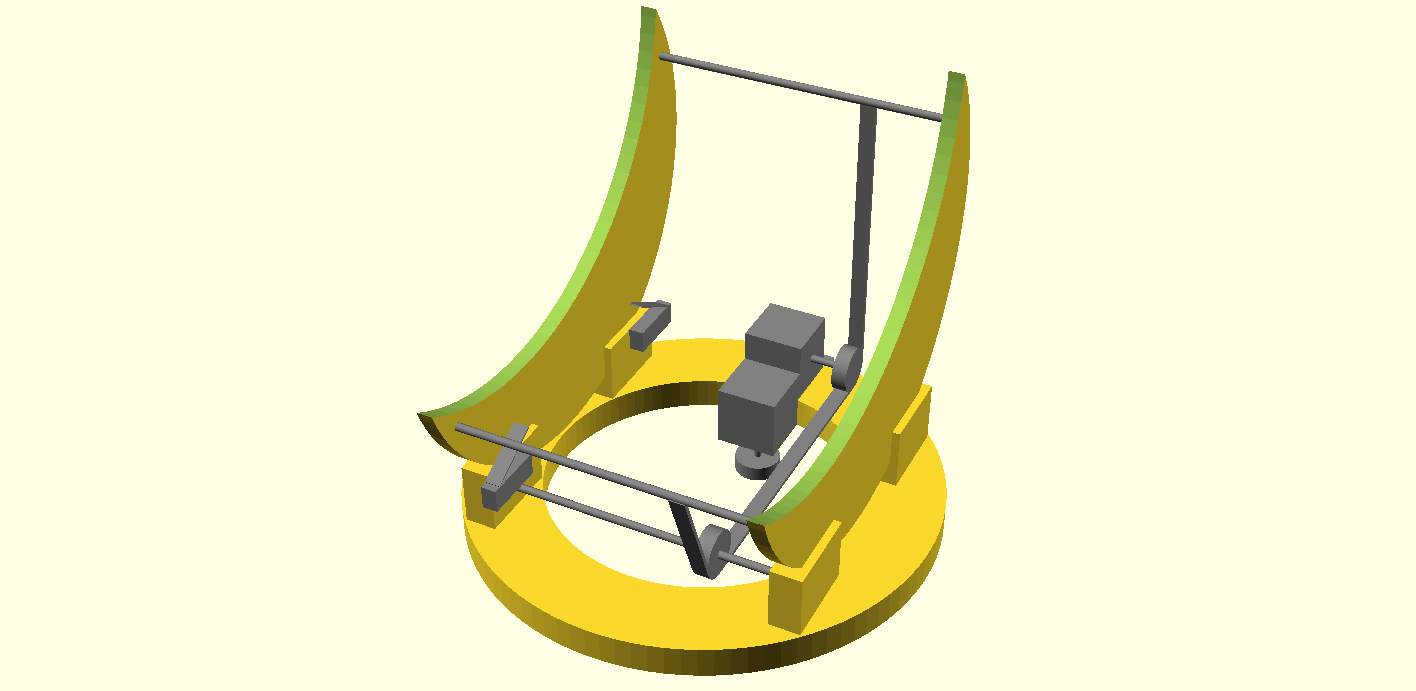
\includegraphics[width=0.9\linewidth]{\figures/OpenSCAD/elev3.png}
    \decoRule
    \caption[
    Schéma du mécanisme permettant un mouvement d'élévation]{
    Schéma du mécanisme permettant un mouvement d'élévation}
    \label{fig:Schéma du mécanisme permettant un mouvement d'élévation}
    \end{figure}

\vspace{1cm}

Quant au zoom, il faudra créer un ensemble de pièces pour maintenir le zoom lui même, la caméra (non représentée), le moteur permettant d'actionner le zoom, les capteurs de positions extrêmes, ainsi qu'un système permettant de régler finement la position de l'oculaire et de la caméra.

Un cran pour activer les capteurs de positions extrêmes pourrait être fixé à l'oculaire avec un collier de serrage par exemple.

\begin{figure}[H]
    \centering
    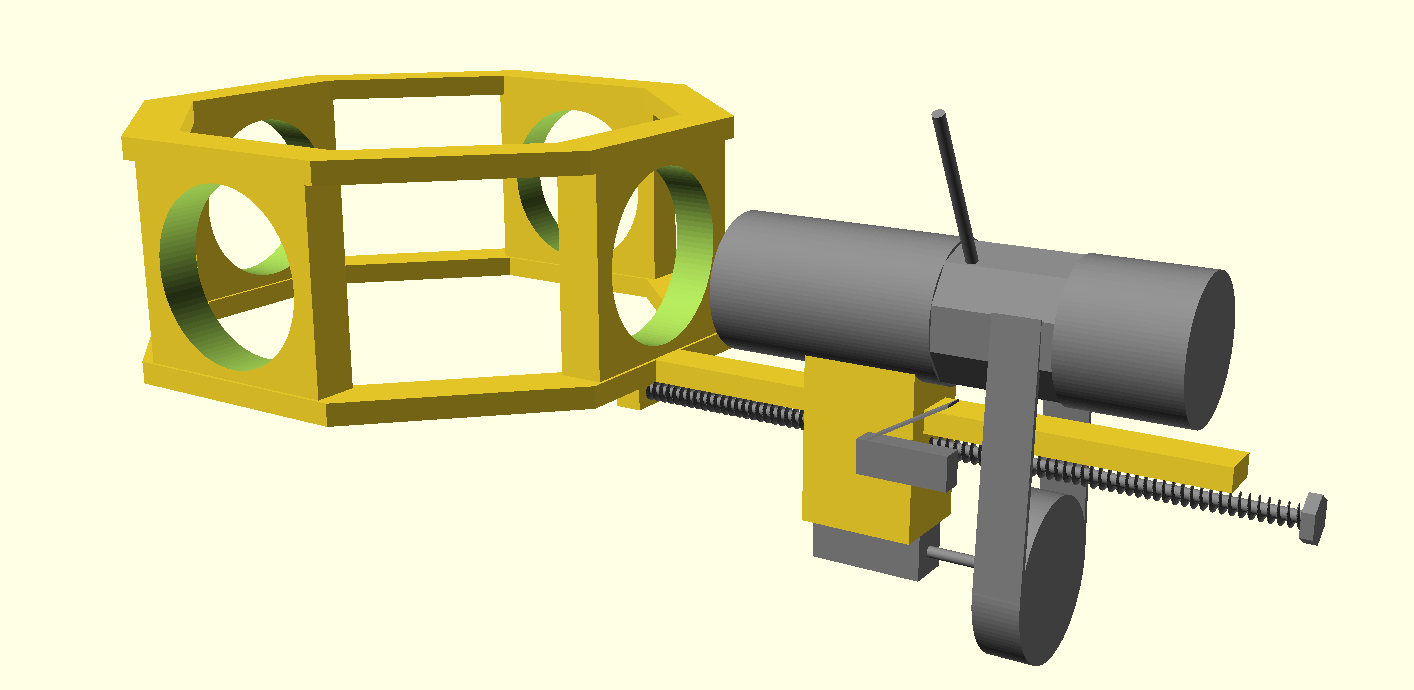
\includegraphics[width=0.9\linewidth]{\figures/OpenSCAD/zoom.png}
    \decoRule
    \caption[
    Schéma du mécanisme permettant un mouvement du zoom]{
    Schéma du mécanisme permettant un mouvement du zoom}
    \label{fig:Schéma du mécanisme permettant un mouvement du zoom}
    \end{figure}

\section{État actuel de la structure}

Pour l'instant nous avons imprimé toutes les pièces fournies par le projet original. Certaines ont subi une détérioration de la qualité lors de l'impression pour une raison mal connue et demeurent à réimprimer. Le Socle, la plateforme tournante et le support du miroir secondaire ont été montés. Aucune modification de la structure en vue d'y intégrer le système électronique n'a été faite.

\begin{figure}[H]
    \centering
    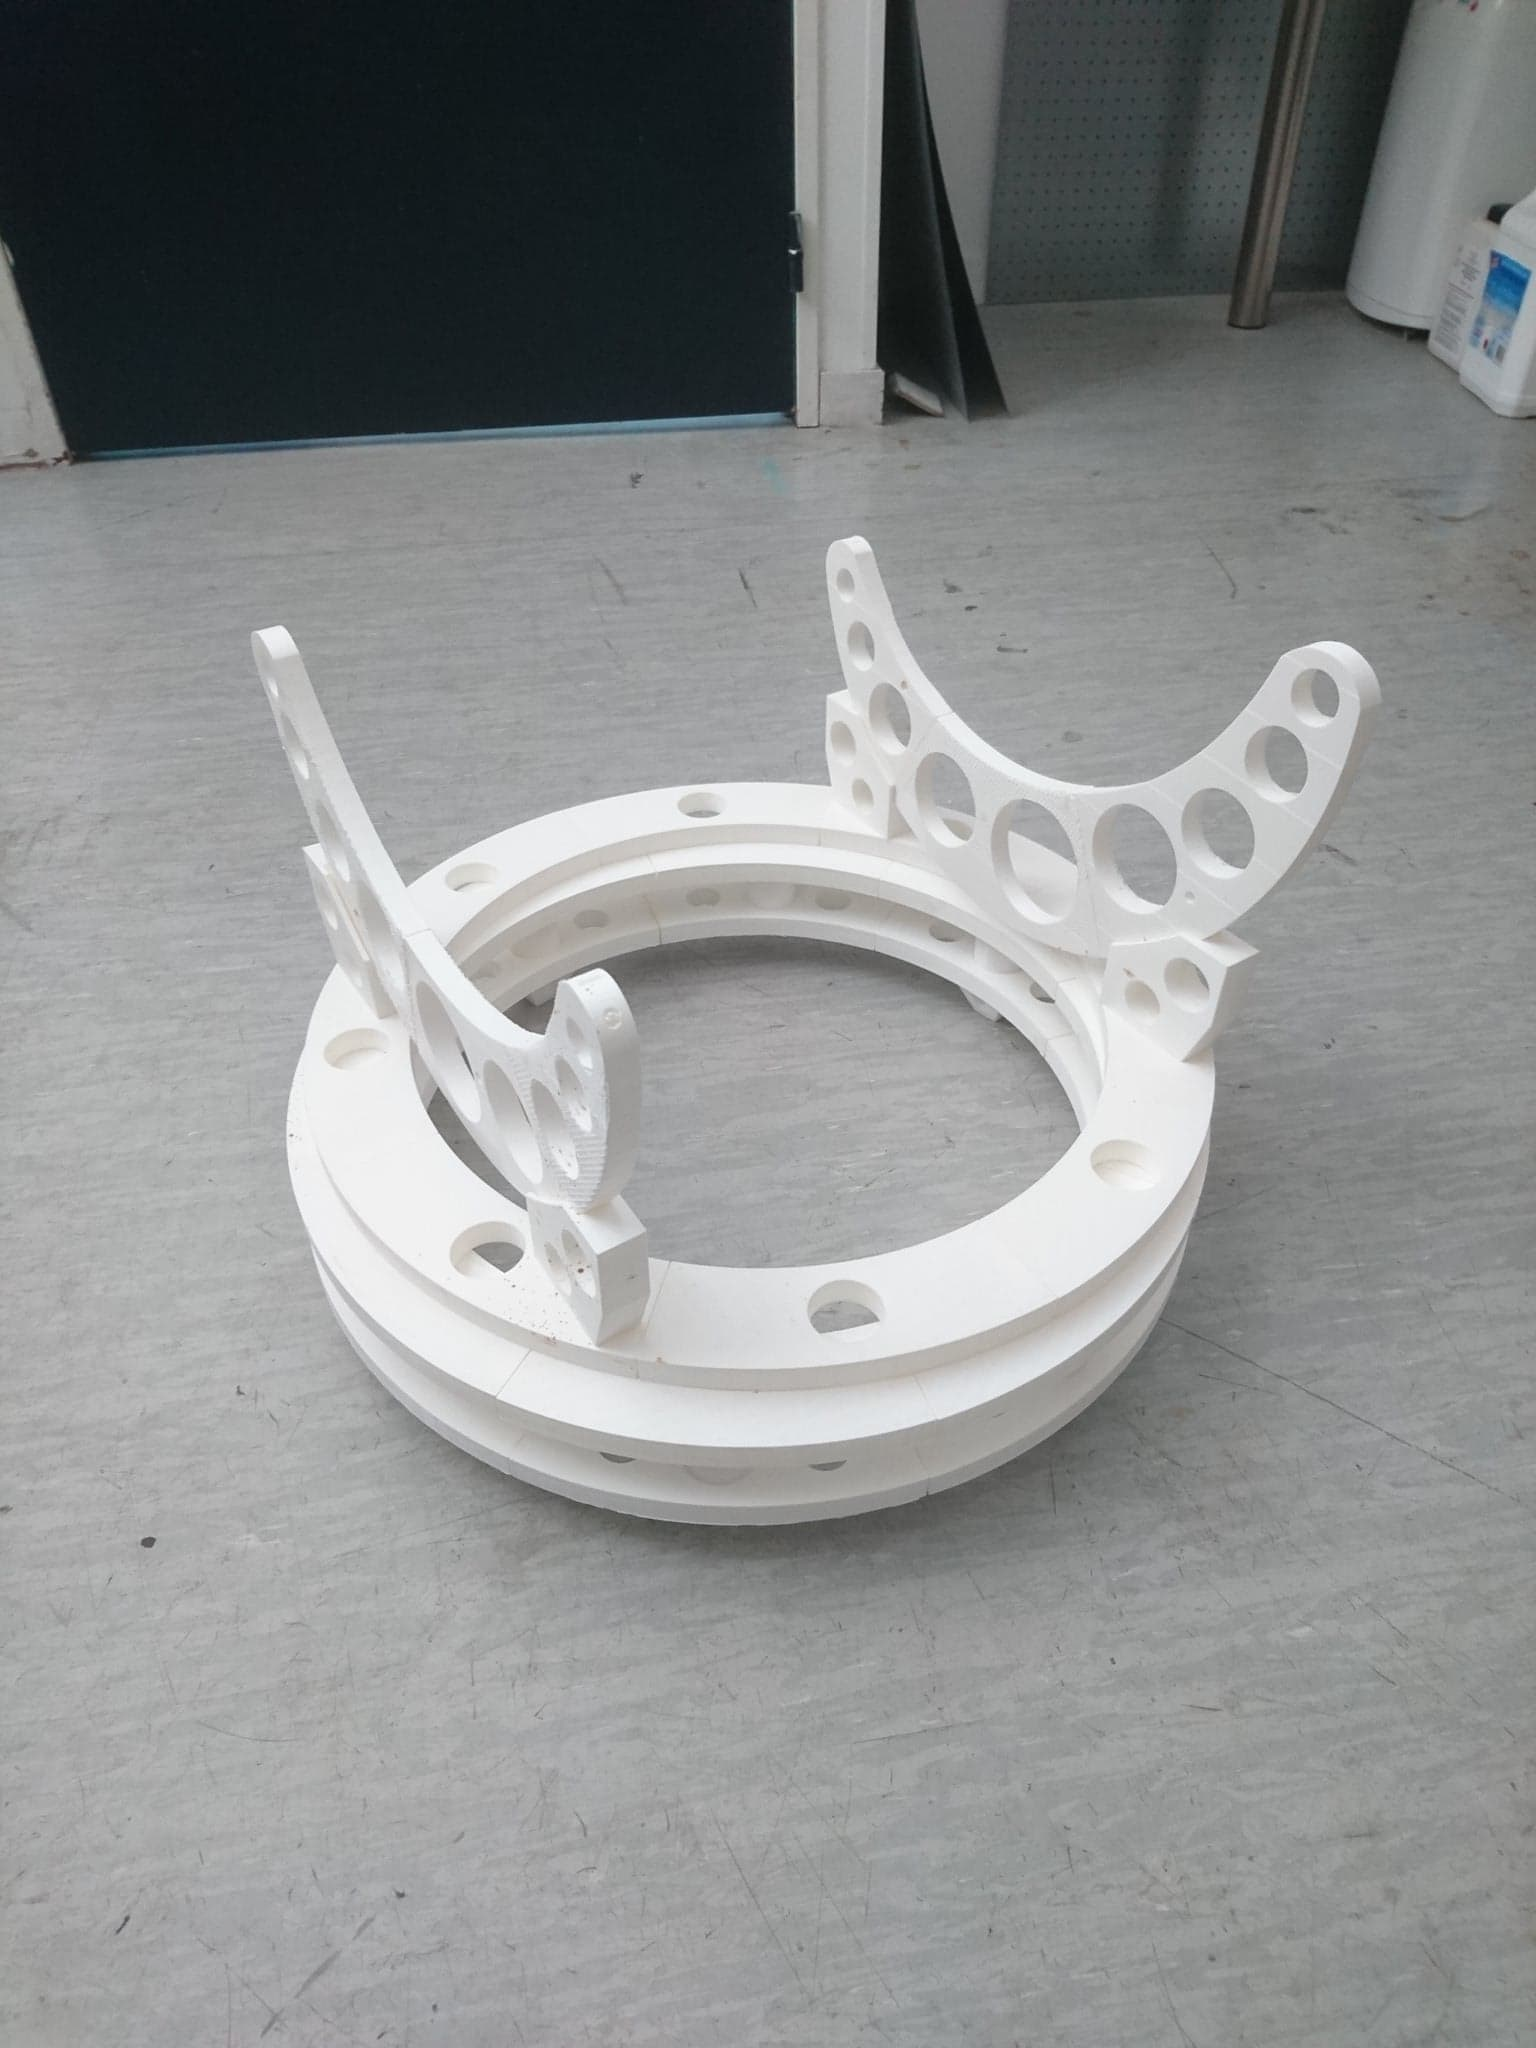
\includegraphics[width=0.3\linewidth]{\figures/photo_structure1.jpg}
    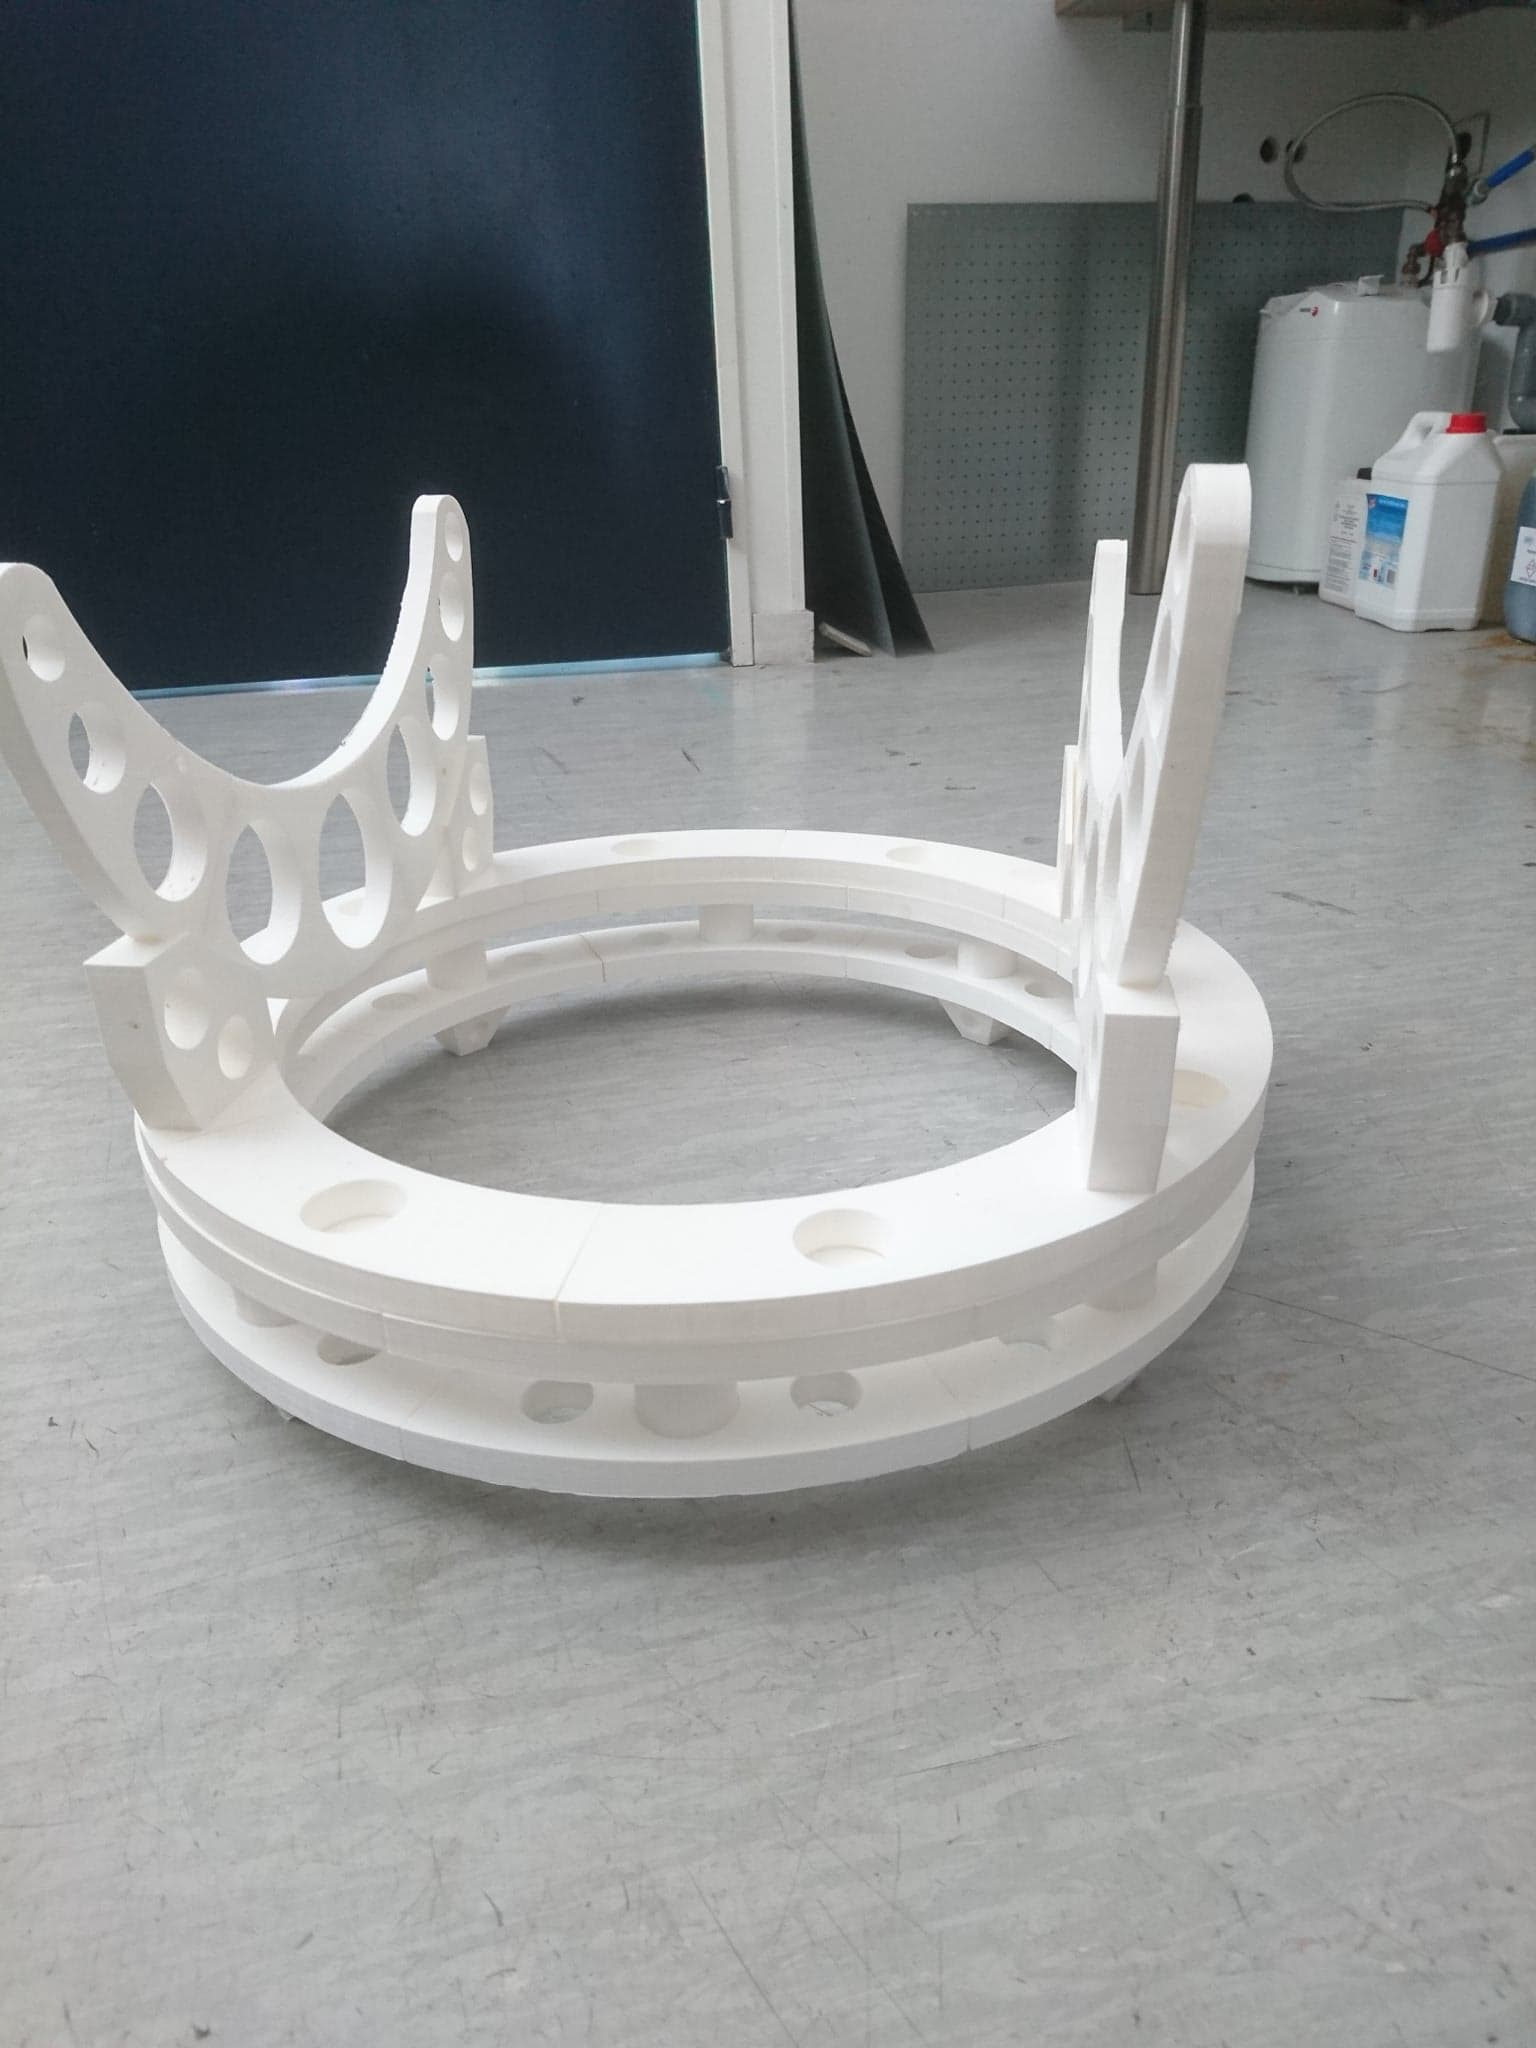
\includegraphics[width=0.3\linewidth]{\figures/photo_structure2.jpg}
    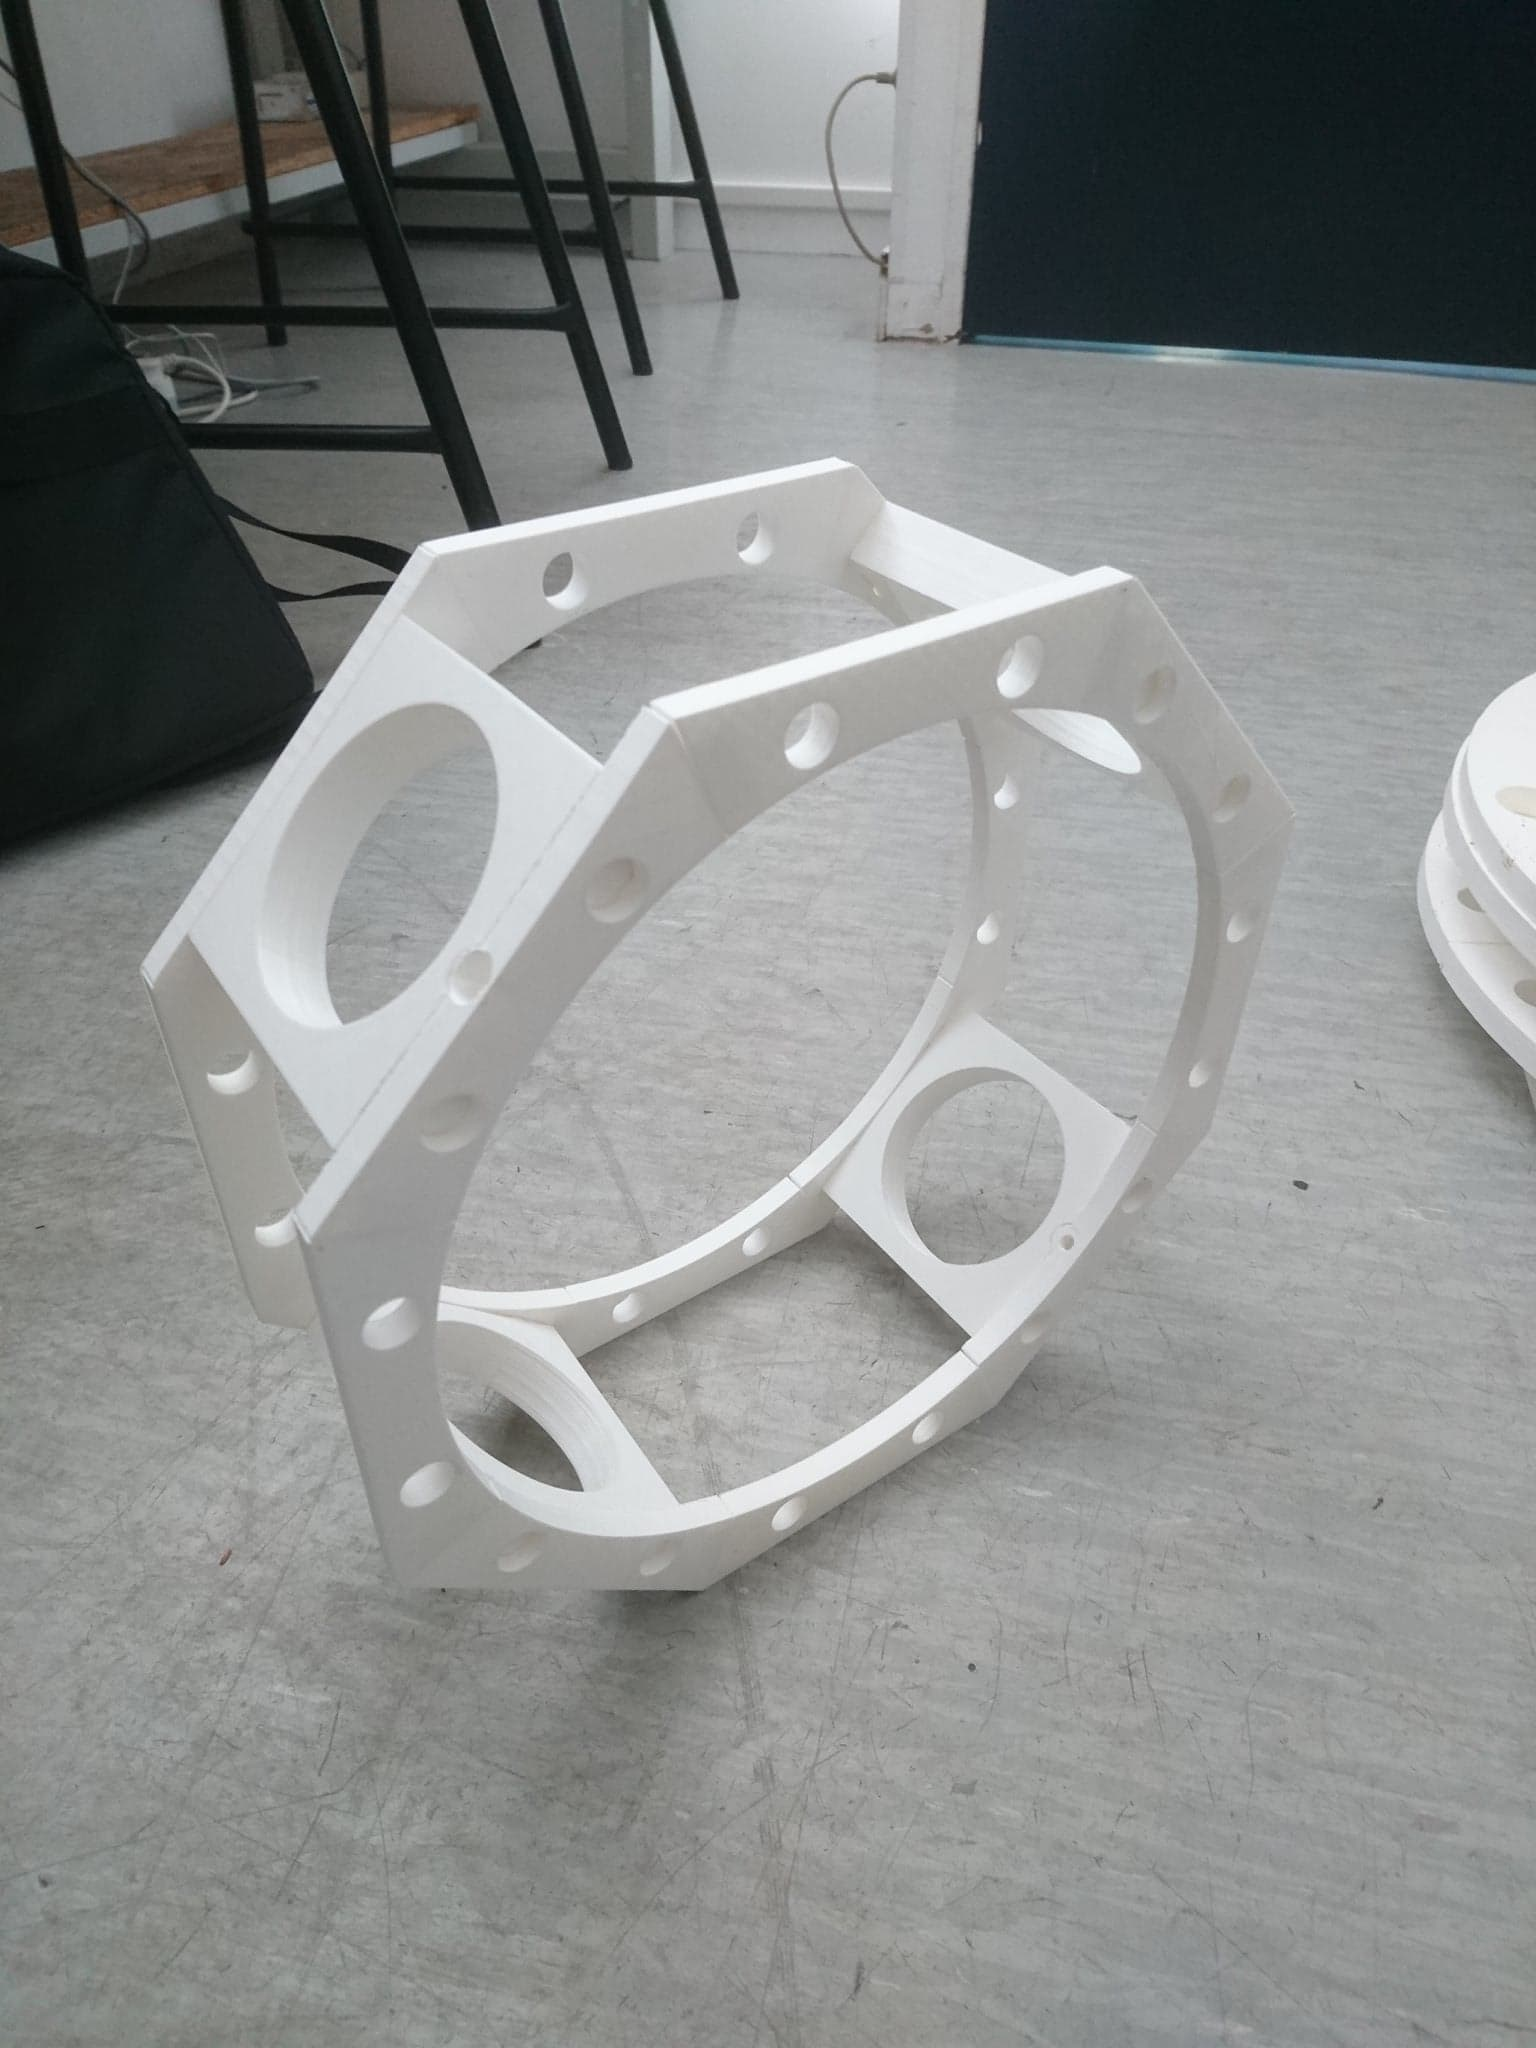
\includegraphics[width=0.3\linewidth]{\figures/photo_structure3.jpg}
    \decoRule
    \caption[
    Photos des parties montées du télescope]{
    Photos des parties montées du télescope}
    \label{fig:Photos des parties montées du télescope}
    \end{figure}


\chapter{Travail restant}

\section{Hardware}

Il reste pour cette partie la fabrication et la validation de la carte, ainsi que le câblage sur le télescope. Ces taches à défaut d'être difficiles sont assez chronophages.

\section{Système d'exploitation}

Le plus urgent est sans doute de réparer la configuration du Hotspot Wifi ainsi que de mettre en place une solution fiable pour transférer le flux vidéo de la caméra.

Ensuite, l'intégration des drivers et du logiciel principal pourront demander quelques configurations au niveau du kernel et du device tree.

Enfin, d'autres taches moins urgentes sont à réaliser, la mise en place d'un pare-feu et la sécurisation du système, la mise en place d'un système de mise à jour, sans doute \codeinline{text}{Mender} ou \codeinline{text}{SWupdate}. Puis diverses optimisations du système d'exploitation, retirer des choses inutiles, comme le daemon gérant le Bluetooth.

\section{Software}

Des travaux de réflexion sur les algorithmes à mettre en place pour mouvoir le télescope et calibrer ses actionneurs ont étés réalisés. Ceux-ci seront à approfondir conjointement aux autres membres du groupe pour écrire le logiciel principal du télescope dont des briques de base apparaissent par différentes extrémités.

\chapter{Organisation}

\section{Planning et répartition du travail}

En raison de l'abandon du projet par Thibaud LE DOLEDEC et Clément AILLOUD partis en stage, le projet ne pourra être mené à terme. Pour aborder la dernière ligne droite avant l'évaluation finale, un choix a donc été fait des tâches sur lesquelles travailler en priorité, au détriment d'autres qui demeureront inachevées.

\vspace{1cm}

Ci-dessous un diagramme représentant l’avancement des différentes tâches du projet. Le gris indique qu’une tâche est terminée ou à un niveau d’avancement satisfaisant et garantissant une maturité proche. Le orange indique les tâches en cours ou prioritaires au moment de l'évaluation finale. Les flèches représentent des liens de dépendance entre certaines tâches.

\begin{figure}[H]
    \centering
	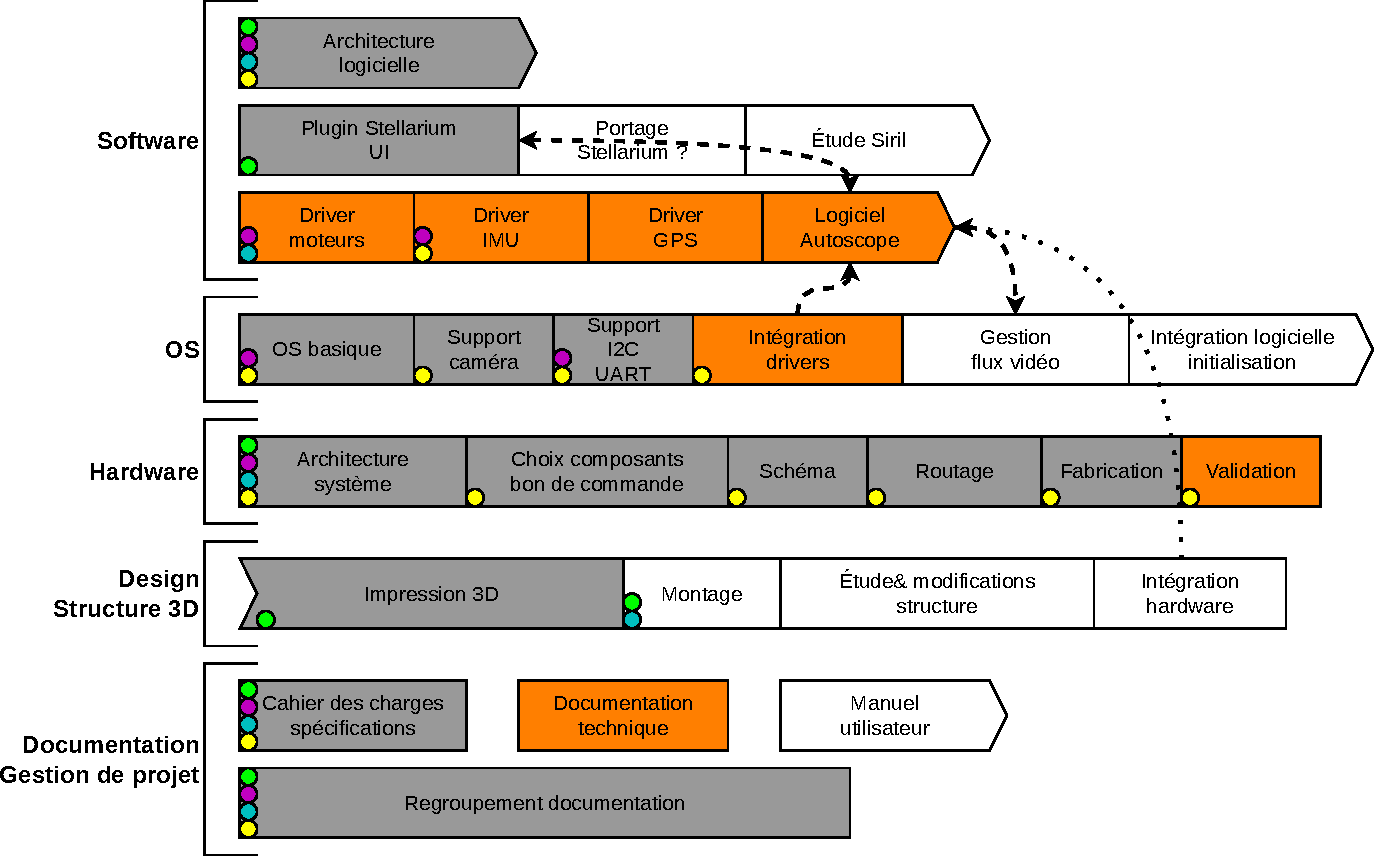
\includegraphics[width=1\linewidth]{\figures/sch_gantt.pdf}
    \decoRule
    \caption[
    Diagramme de l'organisation temporelle du travail sur le projet]{
    Diagramme de l'organisation temporelle du travail sur le projet}
    \label{fig:Diagramme de l'organisation temporelle du travail sur le projet}
    \end{figure}


\section{Accessibilité du projet sur internet}

Le projet étant libre, il est disponible sur Github sous licence GPL-2. Nous tachons d'accompagner nos différents dépôts d'une documentation claire permettant d'obtenir les informations suivantes~:
\begin{itemize}[label=$\bullet$]
	\item Une description brève et précise sur le contenu du dépôt et son rôle au sein du projet.
	\item Une explication de la procédure à suivre pour utiliser le contenu du dépôt.
	\item Une explication de la procédure à suivre pour travailler sur le dépôt.
	\end{itemize}

\subsection{Dépôt principal}

\url{https://github.com/thibaudledo/Autoscope}

\vspace{1cm}

Le dépôt est organisé comme suit~:
\begin{itemize}[label=$\bullet$]
	\item Branche {\href{https://github.com/thibaudledo/Autoscope/tree/master}{\codeinline{text}{master}}}~: Sources du logiciel principal et explications sur le projet dans son ensemble.
	\item Release {\href{https://github.com/thibaudledo/Autoscope/releases}{\codeinline{text}{alpha}}}~: Paquets et fichiers binaires pour utiliser le projet "out of the box" (release expérimentale).
	\item Branche {\href{https://github.com/thibaudledo/Autoscope/tree/hardware}{\codeinline{text}{hardware}}}~: Fichiers Blender de la structure du télescope et fichiers KiCad de la carte électronique du projet.
	\item Branche {\href{https://github.com/thibaudledo/Autoscope/tree/doc}{\codeinline{text}{doc}}}~: Documentations et datasheets des composants et éléments utilisés pour le projet.
	\item Branche {\href{https://github.com/thibaudledo/Autoscope/tree/latex}{\codeinline{text}{latex}}}~: Fichiers LaTex et \codeinline{text}{.pdf} des comptes rendus sur le projet.
	\item Branche {\href{https://github.com/thibaudledo/Autoscope/tree/hello_mod}{\codeinline{text}{hello_mod}}}~: Sources d'un driver helloworld servant d'exemple.
	\item Branche {\href{https://github.com/thibaudledo/Autoscope/tree/a4988_mod}{\codeinline{text}{a4988_mod}}}~: Sources du driver des contrôleurs moteur et des capteurs de fin de course des moteurs.
	\item Branche {\href{https://github.com/thibaudledo/Autoscope/tree/mpu9250_mod}{\codeinline{text}{mpu9250_mod}}}~: Sources du driver de la centrale inertielle.
	\item Branche {\href{https://github.com/thibaudledo/Autoscope/tree/mtk3339d}{\codeinline{text}{mtk3339d}}}~: Sources du driver du GPS.
	\end{itemize}

\newpage
\subsection{Dépôt du système d'exploitation de la Raspberry-Pi}

\url{https://github.com/thomaslepoix/meta-autoscope}

\vspace{1cm}

Il s'agit de la couche de métadonnées utilisées par Yocto pour construire le système d'exploitation Linux utilisé par la Raspberry-Pi du télescope. Une image pré-compilée du système d'exploitation figurera sur {\href{https://github.com/thibaudledo/Autoscope/releases}{la release \codeinline{text}{alpha} du dépôt principal}.

\vspace{1cm}

Le dépôt est organisé comme suit~:
\begin{itemize}[label=$\bullet$]
	\item Branche {\href{https://github.com/thomaslepoix/meta-autoscope/tree/rpi}{\codeinline{text}{rpi}}}~: Métadonnées Yocto et explications de comment compiler et installer le système d'exploitation.
	\item Branche {\href{https://github.com/thomaslepoix/meta-autoscope/tree/rpi-repo}{\codeinline{text}{rpi-repo}}}~: Données utilisées par Repo pour synchroniser le dépôt à d'autres dépôts de métadonnées Yocto utilisées pout construire l'OS.
	\end{itemize}

\subsection{Dépôt du plugin de Stellarium}

\url{https://github.com/thibaudledo/Autoscope-Stellarium-plugin}

\vspace{1cm}

Il s'agit du plugin de Stellarium contenant l'interface par laquelle l'utilisateur interagira avec le télescope. Un paquet pré-compilé pour linux de Stellarium incluant le plugin figure sur {\href{https://github.com/thibaudledo/Autoscope/releases}{la release \codeinline{text}{alpha} du dépôt principal}.

\vspace{1cm}

Le dépôt est organisé comme suit~:
\begin{itemize}[label=$\bullet$]
	\item Branche {\href{https://github.com/thibaudledo/Autoscope-Stellarium-plugin/tree/master}{\codeinline{text}{master}}}~: Sources du plugin, patch des sources de Stellarium et explications de comment compiler une version de Stellarium intégrant le plugin.
	\end{itemize}


\part{Thomas ABGRALL}
\chapter{Avancement général}

En raison de l'abandon du projet par Thibaud LE DOLEDEC et Clément AILLOUD partis en stage, le projet ne pourra être mené à terme. Pour aborder la dernière ligne droite avant l'évaluation finale, un choix a donc été fait des taches sur lesquelles travailler en priorité, au détriment d'autres qui demeureront inachevées.

\vspace{1cm}

Ci-dessous un diagramme représentant l’avancement des différentes taches du projet. Le gris indique qu’une tache est terminée ou à un niveau d’avancement satisfaisant et garantissant une maturité proche. Le orange indique les taches sur lesquelles nous travaillerons en priorité avant la fin du projet. Les flèches représentent des liens de dépendance entre les taches.

\begin{figure}[H]
    \centering
	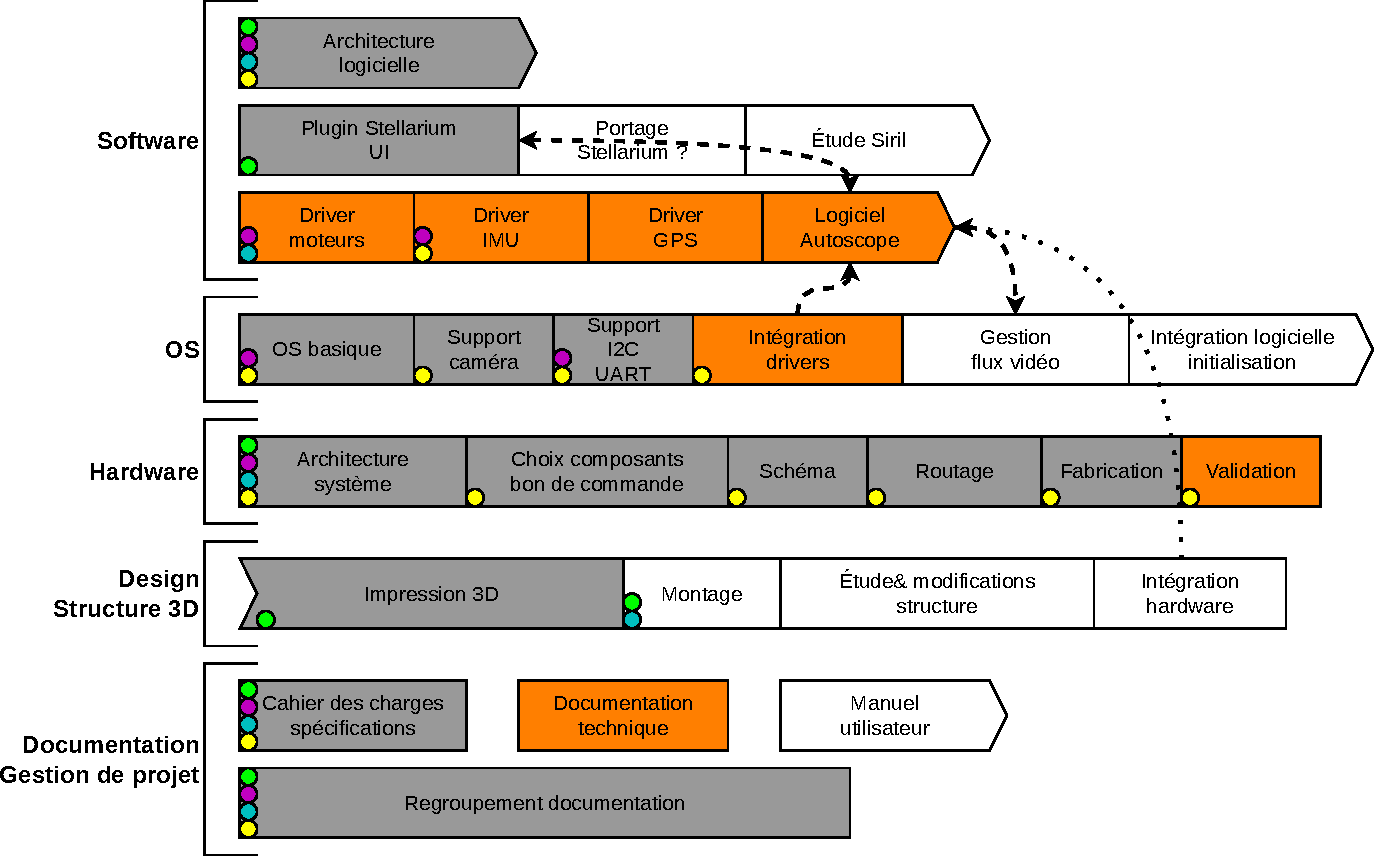
\includegraphics[width=1\linewidth]{\figures/sch_gantt.pdf}
    \decoRule
    \caption[
    Diagramme de l'organisation temporelle du travail sur le projet]{
    Diagramme de l'organisation temporelle du travail sur le projet}
    \label{fig:Diagramme de l'organisation temporelle du travail sur le projet}
    \end{figure}

\section{Prévisions pour le dernier sprint}

Malgré son aspect visuel intéressant pour promouvoir le projet ainsi que de sont aspect central (il s'agit tout de même d'un télescope), le travail sur la structure du télescope sera écarté des taches prioritaires. Cela pour deux raisons~:
\begin{itemize}[label=$\bullet$]
	\item Il s'agit d'une partie du projet demandant beaucoup de temps et d'implications par rapport à ce dont nous disposons. Nous n'aurions sans doute pas le temps de terminer cela avant l'évaluation.
	\item N'ayant ni des connaissances particulières en optique, ni la maîtrise d'un logiciel de modélisation 3D, nous ne sommes pas plus qualifiés qu'une personne aléatoire voulant contribuer au projet. Nous pensons donc qu'il vaut mieux nous concentrer sur des taches faisant partie de notre domaine de qualification, que nous serions capable de réaliser plus facilement ou mieux qu'une personne aléatoire. L'élaboration des drivers correspond typiquement à ce cas.
	\end{itemize}

\vspace{1cm}

Le travail sur les drivers, quant à lui devra être avancé autant que faire se peut. En effet le logiciel principal du télescope dépend lourdement des interfaces avec les drivers et ne peut être commencé tant que les drivers ne sont pas fonctionnels.

De plus, ce logiciel étant la clef de voûte du projet, la finalisation de certaines taches comme certains éléments du plugin Stellarium ou la gestion du flux vidéo au sein de l'OS doit être réalisée conjointement à l'écriture de ce logiciel.

L'absence des ces drivers commence donc à bloquer l'évolution d'autres taches.

\vspace{1cm}

Enfin un travail de documentation devra être fait pour qu'il soit possible à une personne future (nous-mêmes ou qui que ce soit) de travailler sur ce projet ou de réutiliser notre travail.





\chapter{Accessibilité au projet sur internet}

Le projet étant libre, il est disponible sur Github sous licence GPL-2. Nous tachons d'accompagner nos différents dépôts d'une documentation claire permettant d'obtenir les informations suivantes~:
\begin{itemize}[label=$\bullet$]
	\item Une description brève et précise sur le contenu du dépôt et son rôle au sein du projet.
	\item Une explication de la procédure à suivre pour utiliser le contenu du dépôt.
	\item Une explication de la procédure à suivre pour travailler sur le dépôt.
	\end{itemize}

\section{Dépôt principal}

\url{https://github.com/thibaudledo/Autoscope}

\vspace{1cm}

Le dépôt est organisé comme suit~:
\begin{itemize}[label=$\bullet$]
	\item Branche {\href{https://github.com/thibaudledo/Autoscope/tree/master}{\codeinline{text}{master}}}~: Licence du projet et explications sur le projet dans son ensemble.
	\item Release {\href{https://github.com/thibaudledo/Autoscope/releases}{\codeinline{text}{alpha}}}~: Paquets et fichiers binaires pour utiliser le projet "out of the box" (release expérimentale).
	\item Branche {\href{https://github.com/thibaudledo/Autoscope/tree/hardware}{\codeinline{text}{hardware}}}~: Fichiers Blender de la structure du télescope et fichiers KiCad de la carte électronique du projet.
	\item Branche {\href{https://github.com/thibaudledo/Autoscope/tree/doc}{\codeinline{text}{doc}}}~: Documentations et datasheets des composants et éléments utilisés pour le projet.
	\item Branche {\href{https://github.com/thibaudledo/Autoscope/tree/latex}{\codeinline{text}{latex}}}~: Fichiers LaTex et \codeinline{text}{.pdf} des comptes rendus sur le projet.
	\item Branche {\href{https://github.com/thibaudledo/Autoscope/tree/hello_mod}{\codeinline{text}{hello_mod}}}~: Sources d'un driver helloworld servant d'exemple.
	\item Branche {\href{https://github.com/thibaudledo/Autoscope/tree/a4988_mod}{\codeinline{text}{a4988_mod}}}~: Sources du driver des contrôleurs moteur et des capteurs de fin de course des moteurs.
	\item Branche {\href{https://github.com/thibaudledo/Autoscope/tree/mpu_9250_mod}{\codeinline{text}{mpu_9250_mod}}}~: Sources du driver de la centrale inertielle.
	\item Branche {\href{https://github.com/thibaudledo/Autoscope/tree/mtk3339_mod}{\codeinline{text}{mtk3339_mod}}}~: Sources du driver du GPS.
	\end{itemize}

\newpage
\section{Dépôt du système d'exploitation de la Raspberry-Pi}

\url{https://github.com/thomaslepoix/meta-autoscope}

\vspace{1cm}

Il s'agit de la couche de métadonnées utilisées par Yocto pour construire le système d'exploitation Linux utilisé par la Raspberry-Pi du télescope. Une image pré-compilée du système d'exploitation figurera sur {\href{https://github.com/thibaudledo/Autoscope/releases}{la release \codeinline{text}{alpha} du dépôt principal}.

\vspace{1cm}

Le dépôt est organisé comme suit~:
\begin{itemize}[label=$\bullet$]
	\item Branche {\href{https://github.com/thomaslepoix/meta-autoscope/tree/rpi}{\codeinline{text}{rpi}}}~: Métadonnées Yocto et explications de comment compiler et installer le système d'exploitation.
	\item Branche {\href{https://github.com/thomaslepoix/meta-autoscope/tree/rpi-repo}{\codeinline{text}{rpi-repo}}}~: Données utilisées par Repo pour synchroniser le dépôt à d'autres dépôts de métadonnées Yocto utilisées pout construire l'OS.
	\end{itemize}

\section{Dépôt du plugin de Stellarium}

\url{https://github.com/thibaudledo/Autoscope-Stellarium-plugin}

\vspace{1cm}

Il s'agit du plugin de Stellarium contenant l'interface par laquelle l'utilisateur interagira avec le télescope. Un paquet pré-compilé pour linux de Stellarium incluant le plugin figure sur {\href{https://github.com/thibaudledo/Autoscope/releases}{la release \codeinline{text}{alpha} du dépôt principal}.

\vspace{1cm}

Le dépôt est organisé comme suit~:
\begin{itemize}[label=$\bullet$]
	\item Branche {\href{https://github.com/thibaudledo/Autoscope-Stellarium-plugin/tree/master}{\codeinline{text}{master}}}~: Sources du plugin, patch des sources de Stellarium et explications de comment compiler une version de Stellarium intégrant le plugin.
	\end{itemize}


\chapter{Structure du télescope}

\section{Projet d'origine}

La structure du télescope est imprimable à l'imprimante 3D et provient d'un projet open source entre temps disparu d'internet~:
\url{https://blog.dagoma.fr/telescope-imprime-en-3d/}

\vspace{1cm}

Voici l'allure du télescope monté. Les barres métalliques raccordant le support du miroir secondaire au reste du télescope sont des barres de camping achetées en magasin de sport.

\begin{figure}[H]
    \centering
    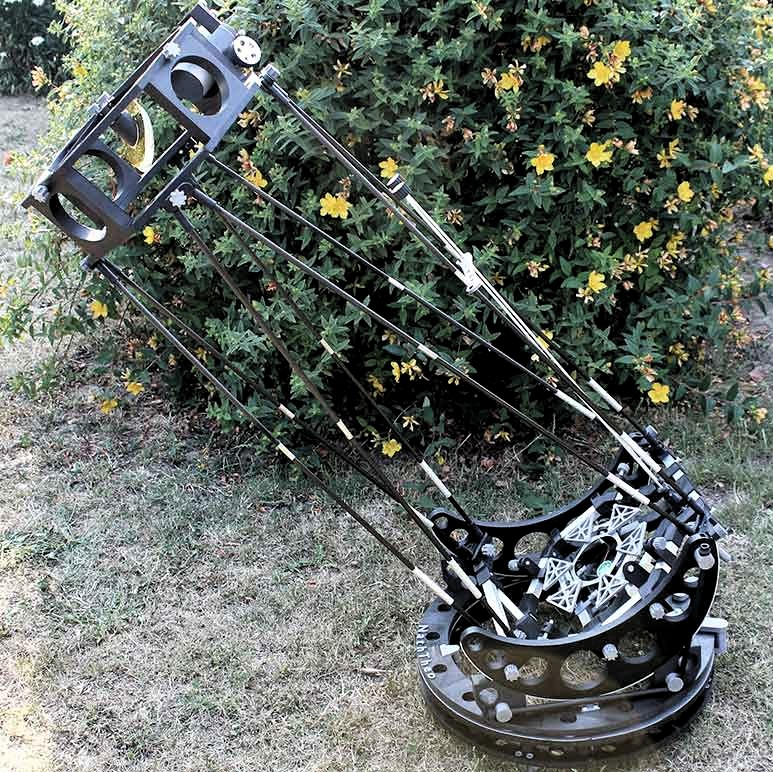
\includegraphics[width=0.5\linewidth]{\figures/photo_telescope2.jpg}
    \decoRule
    \caption[
    Photo du télescope]{
    Photo du télescope}
    \label{fig:Photo du télescope}
    \end{figure}

\begin{figure}[H]
    \centering
    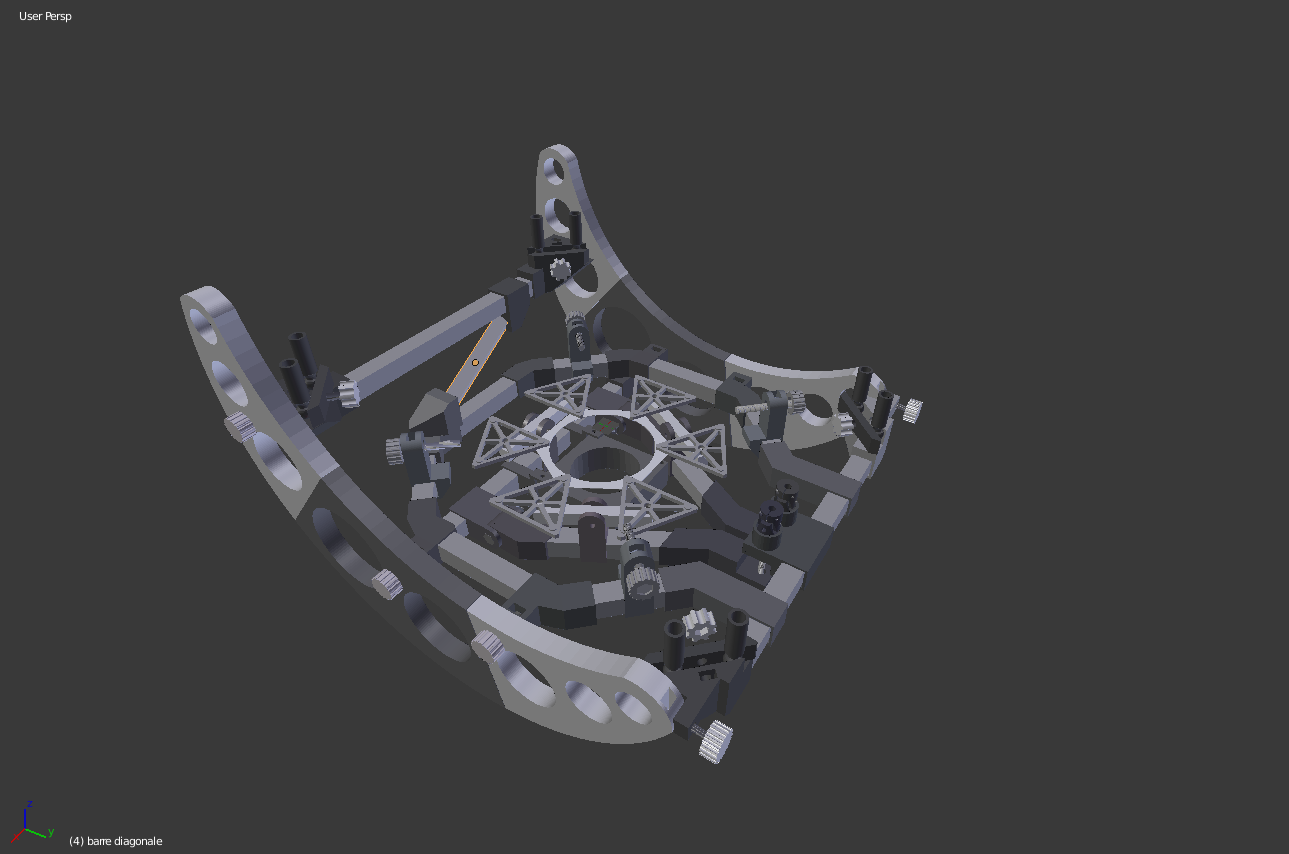
\includegraphics[width=0.49\linewidth]{\figures/blender_3.png}
    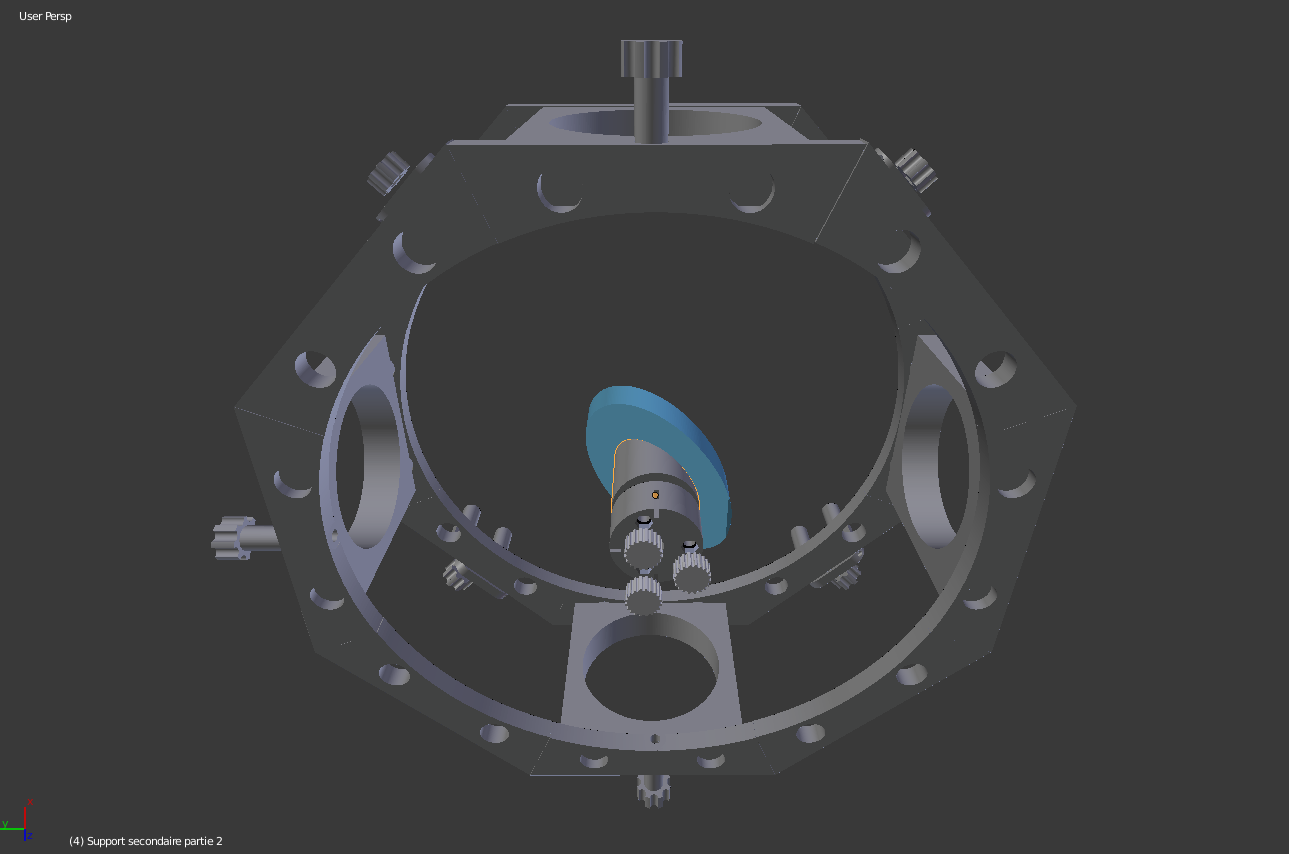
\includegraphics[width=0.49\linewidth]{\figures/blender_4.png}
    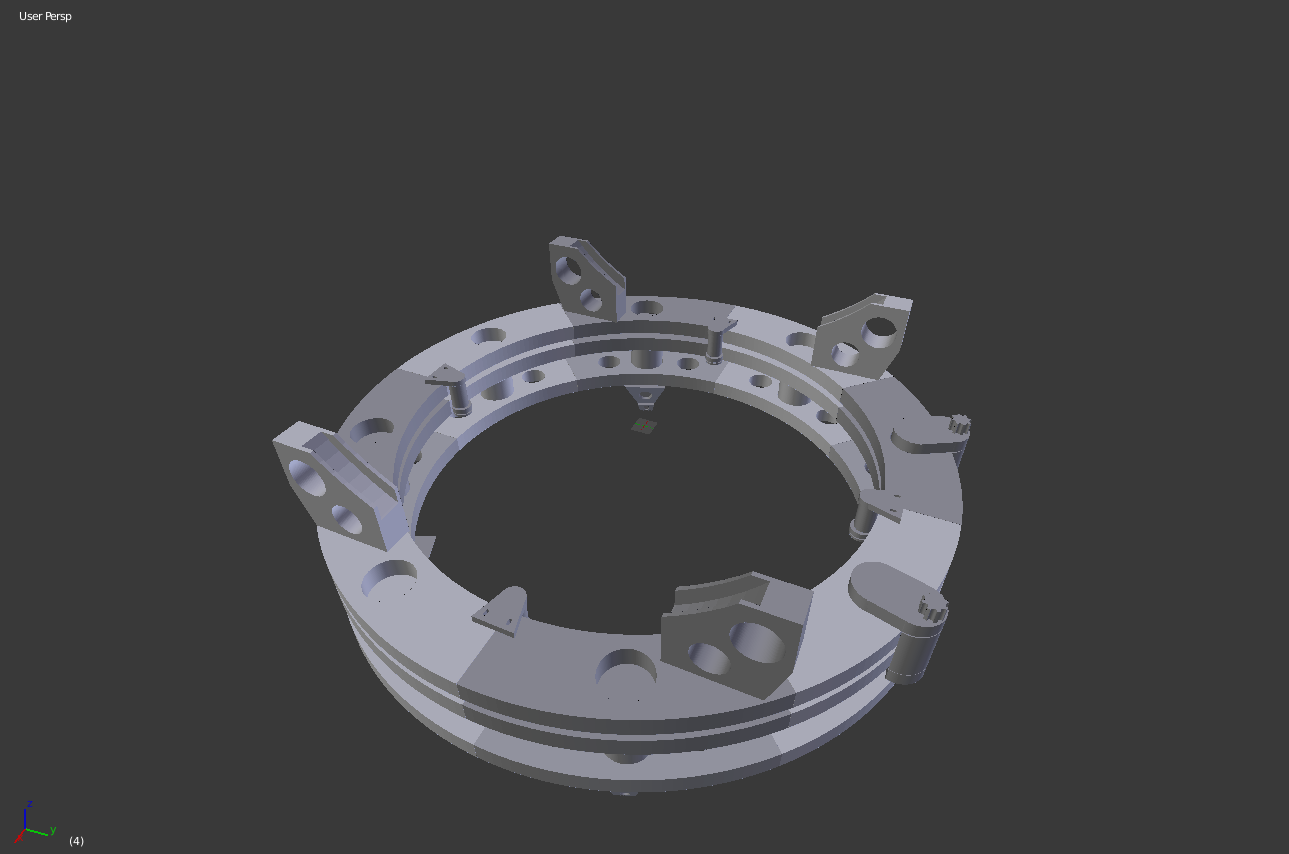
\includegraphics[width=0.49\linewidth]{\figures/blender_5.png}
    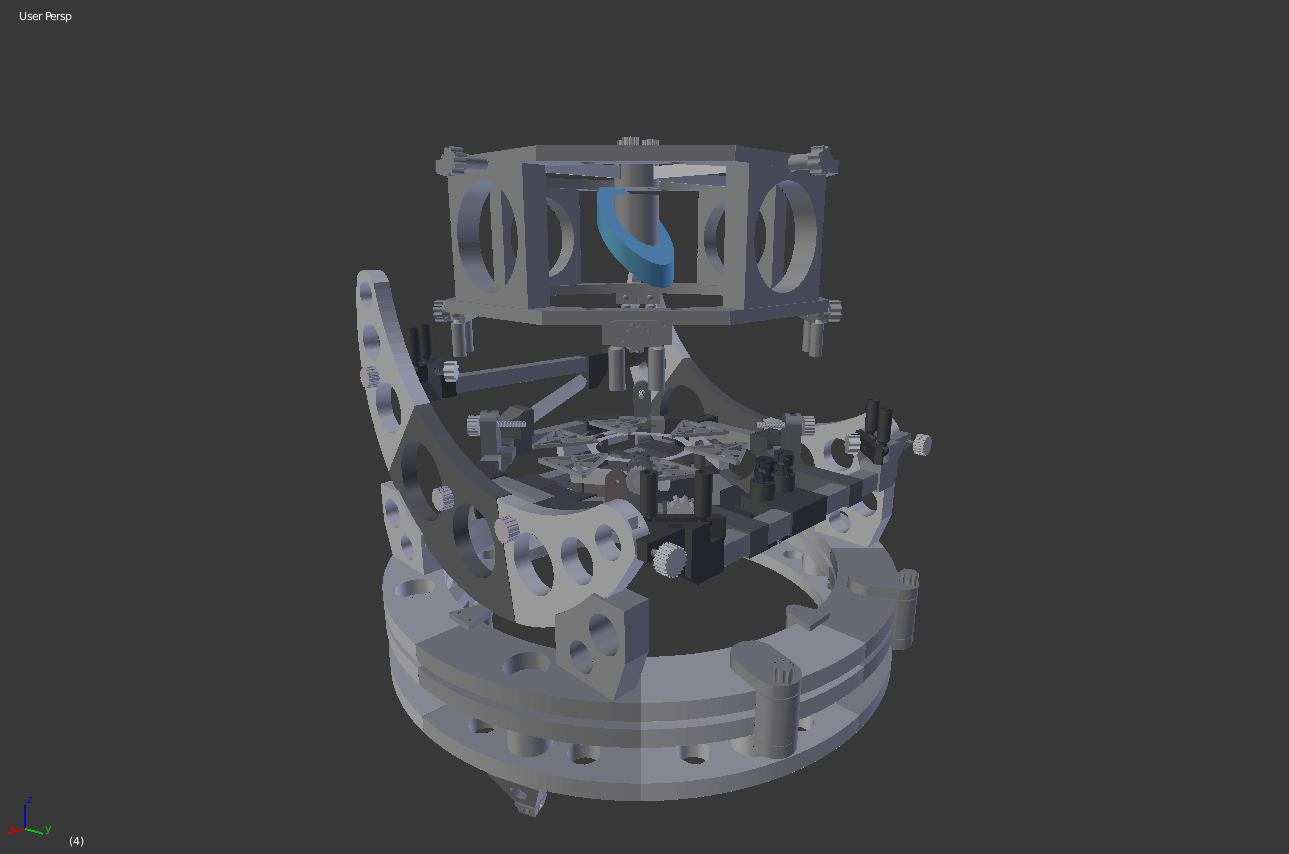
\includegraphics[width=0.49\linewidth]{\figures/blender_6.png}
    \decoRule
    \caption[
    Aperçu des fichiers de production du télescope]{
    Aperçu des fichiers de production du télescope}
    \label{fig:Aperçu des fichiers de production du télescope}
    \end{figure}

\section{Étude de la robotisation du télescope}

Ci-dessous quelques schémas représentant les modifications, telles qu'imaginées, à apporter à la structure du télescope pour l'automatiser.

\vspace{1cm}

Le socle, immobile, sera doté d'une courroie ainsi que d'un cran permettant d'activer le capteur de position. Le système électronique sera solidaire du support du miroir primaire, mobile, à l'étage supérieur. Un moteur doté d'une roue crantée fixé sur la plateforme tournante permettra de la mettre en mouvement par rapport au socle.

\begin{figure}[H]
    \centering
    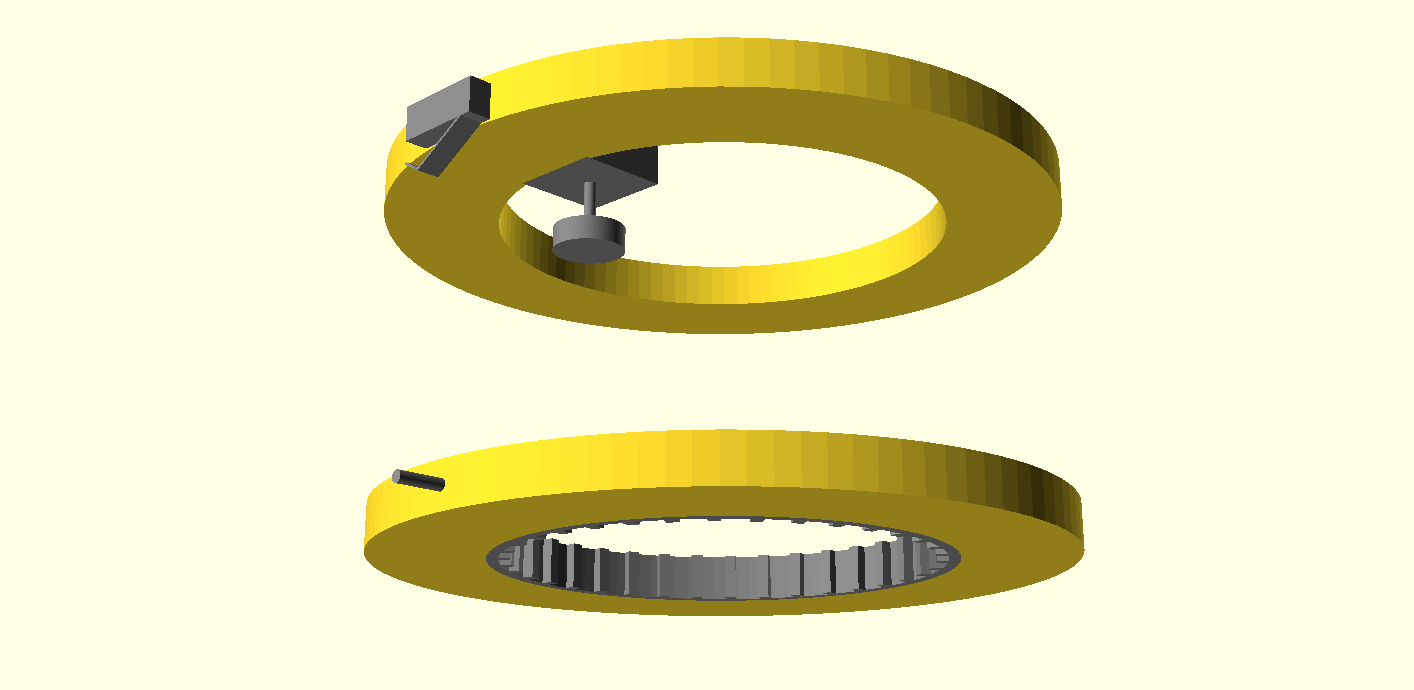
\includegraphics[width=0.9\linewidth]{\figures/OpenSCAD/azim.png}
    \decoRule
    \caption[
    Schéma du mécanisme permettant un mouvement azimutal]{
    Schéma du mécanisme permettant un mouvement azimutal}
    \label{fig:Schéma du mécanisme permettant un mouvement azimutal}
    \end{figure}

\vspace{1cm}

Pour le mouvement d'élévation, un système de tringlerie et de courroie a été imaginé pour mouvoir le support du miroir primaire par rapport à la plateforme tournante. Deux capteurs de position judicieusement placés permettront de détecter lorsque le mouvement atteint l'un de ses maximums.

\begin{figure}[H]
    \centering
    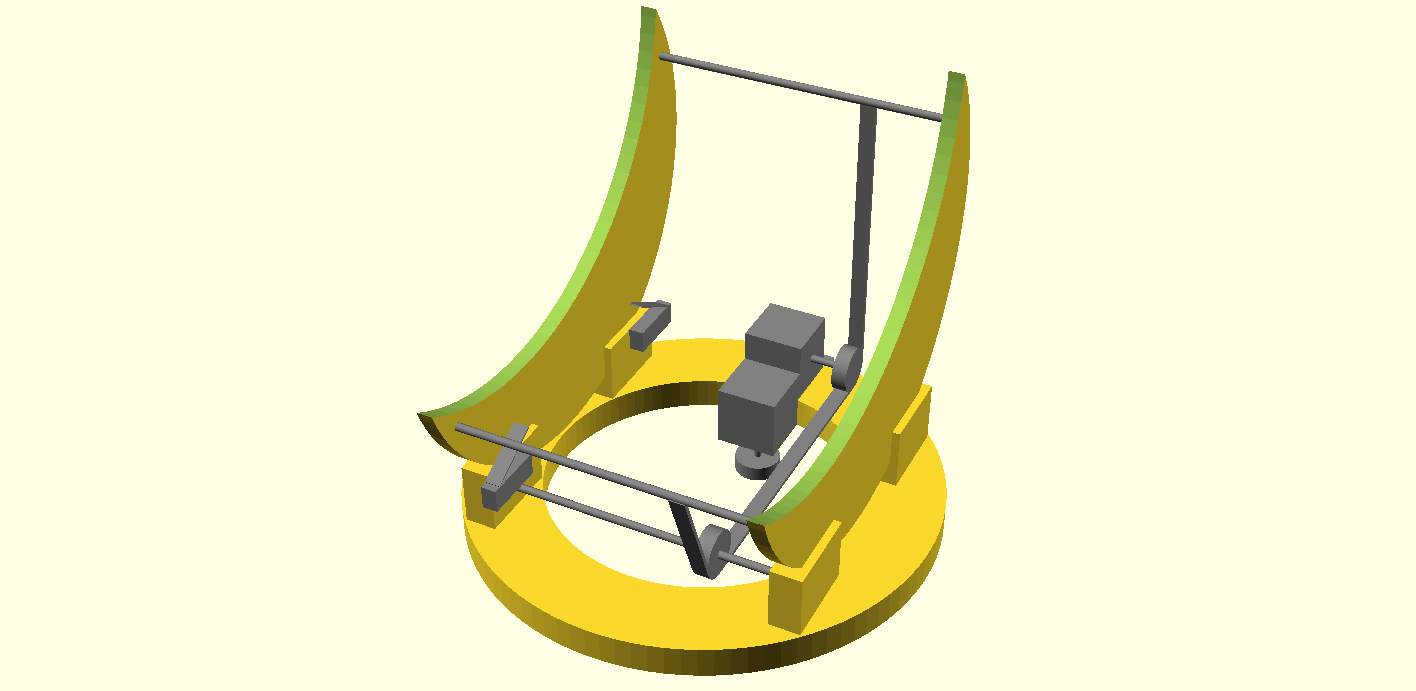
\includegraphics[width=0.9\linewidth]{\figures/OpenSCAD/elev3.png}
    \decoRule
    \caption[
    Schéma du mécanisme permettant un mouvement d'élévation]{
    Schéma du mécanisme permettant un mouvement d'élévation}
    \label{fig:Schéma du mécanisme permettant un mouvement d'élévation}
    \end{figure}

\vspace{1cm}

Quant au zoom, il faudra créer un ensemble de pièces pour maintenir le zoom lui même, la caméra (non représentée), le moteur permettant d'actionner le zoom, les capteurs de positions extrêmes, ainsi qu'un système permettant de régler finement la position de l'oculaire et de la caméra.

Un cran pour activer les capteurs de positions extrêmes pourrait être fixé à l'oculaire avec un collier de serrage par exemple.

\begin{figure}[H]
    \centering
    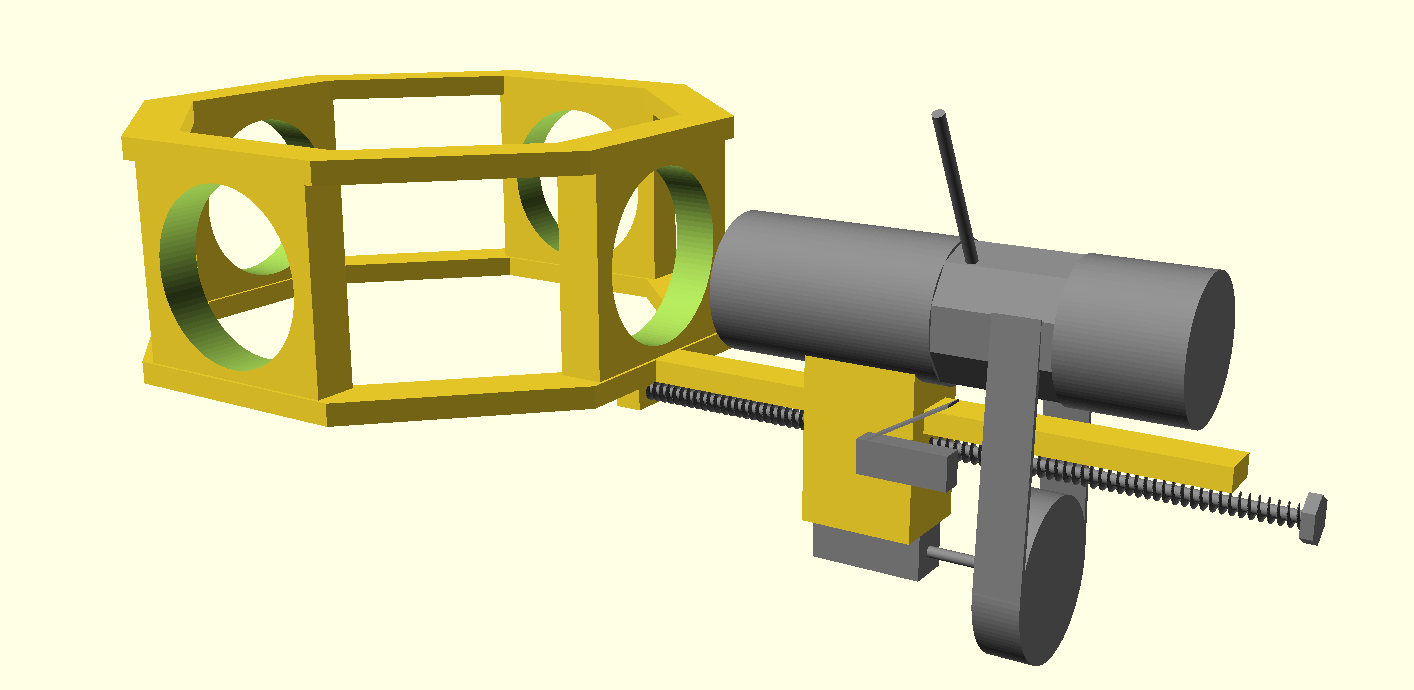
\includegraphics[width=0.9\linewidth]{\figures/OpenSCAD/zoom.png}
    \decoRule
    \caption[
    Schéma du mécanisme permettant un mouvement du zoom]{
    Schéma du mécanisme permettant un mouvement du zoom}
    \label{fig:Schéma du mécanisme permettant un mouvement du zoom}
    \end{figure}

\section{État actuel de la structure}

Pour l'instant nous avons imprimé toutes les pièces fournies par le projet original. Certaines ont subi une détérioration de la qualité lors de l'impression pour une raison mal connue et demeurent à réimprimer. Le Socle, la plateforme tournante et le support du miroir secondaire ont été montés. Aucune modification de la structure en vue d'y intégrer le système électronique n'a été faite.

\begin{figure}[H]
    \centering
    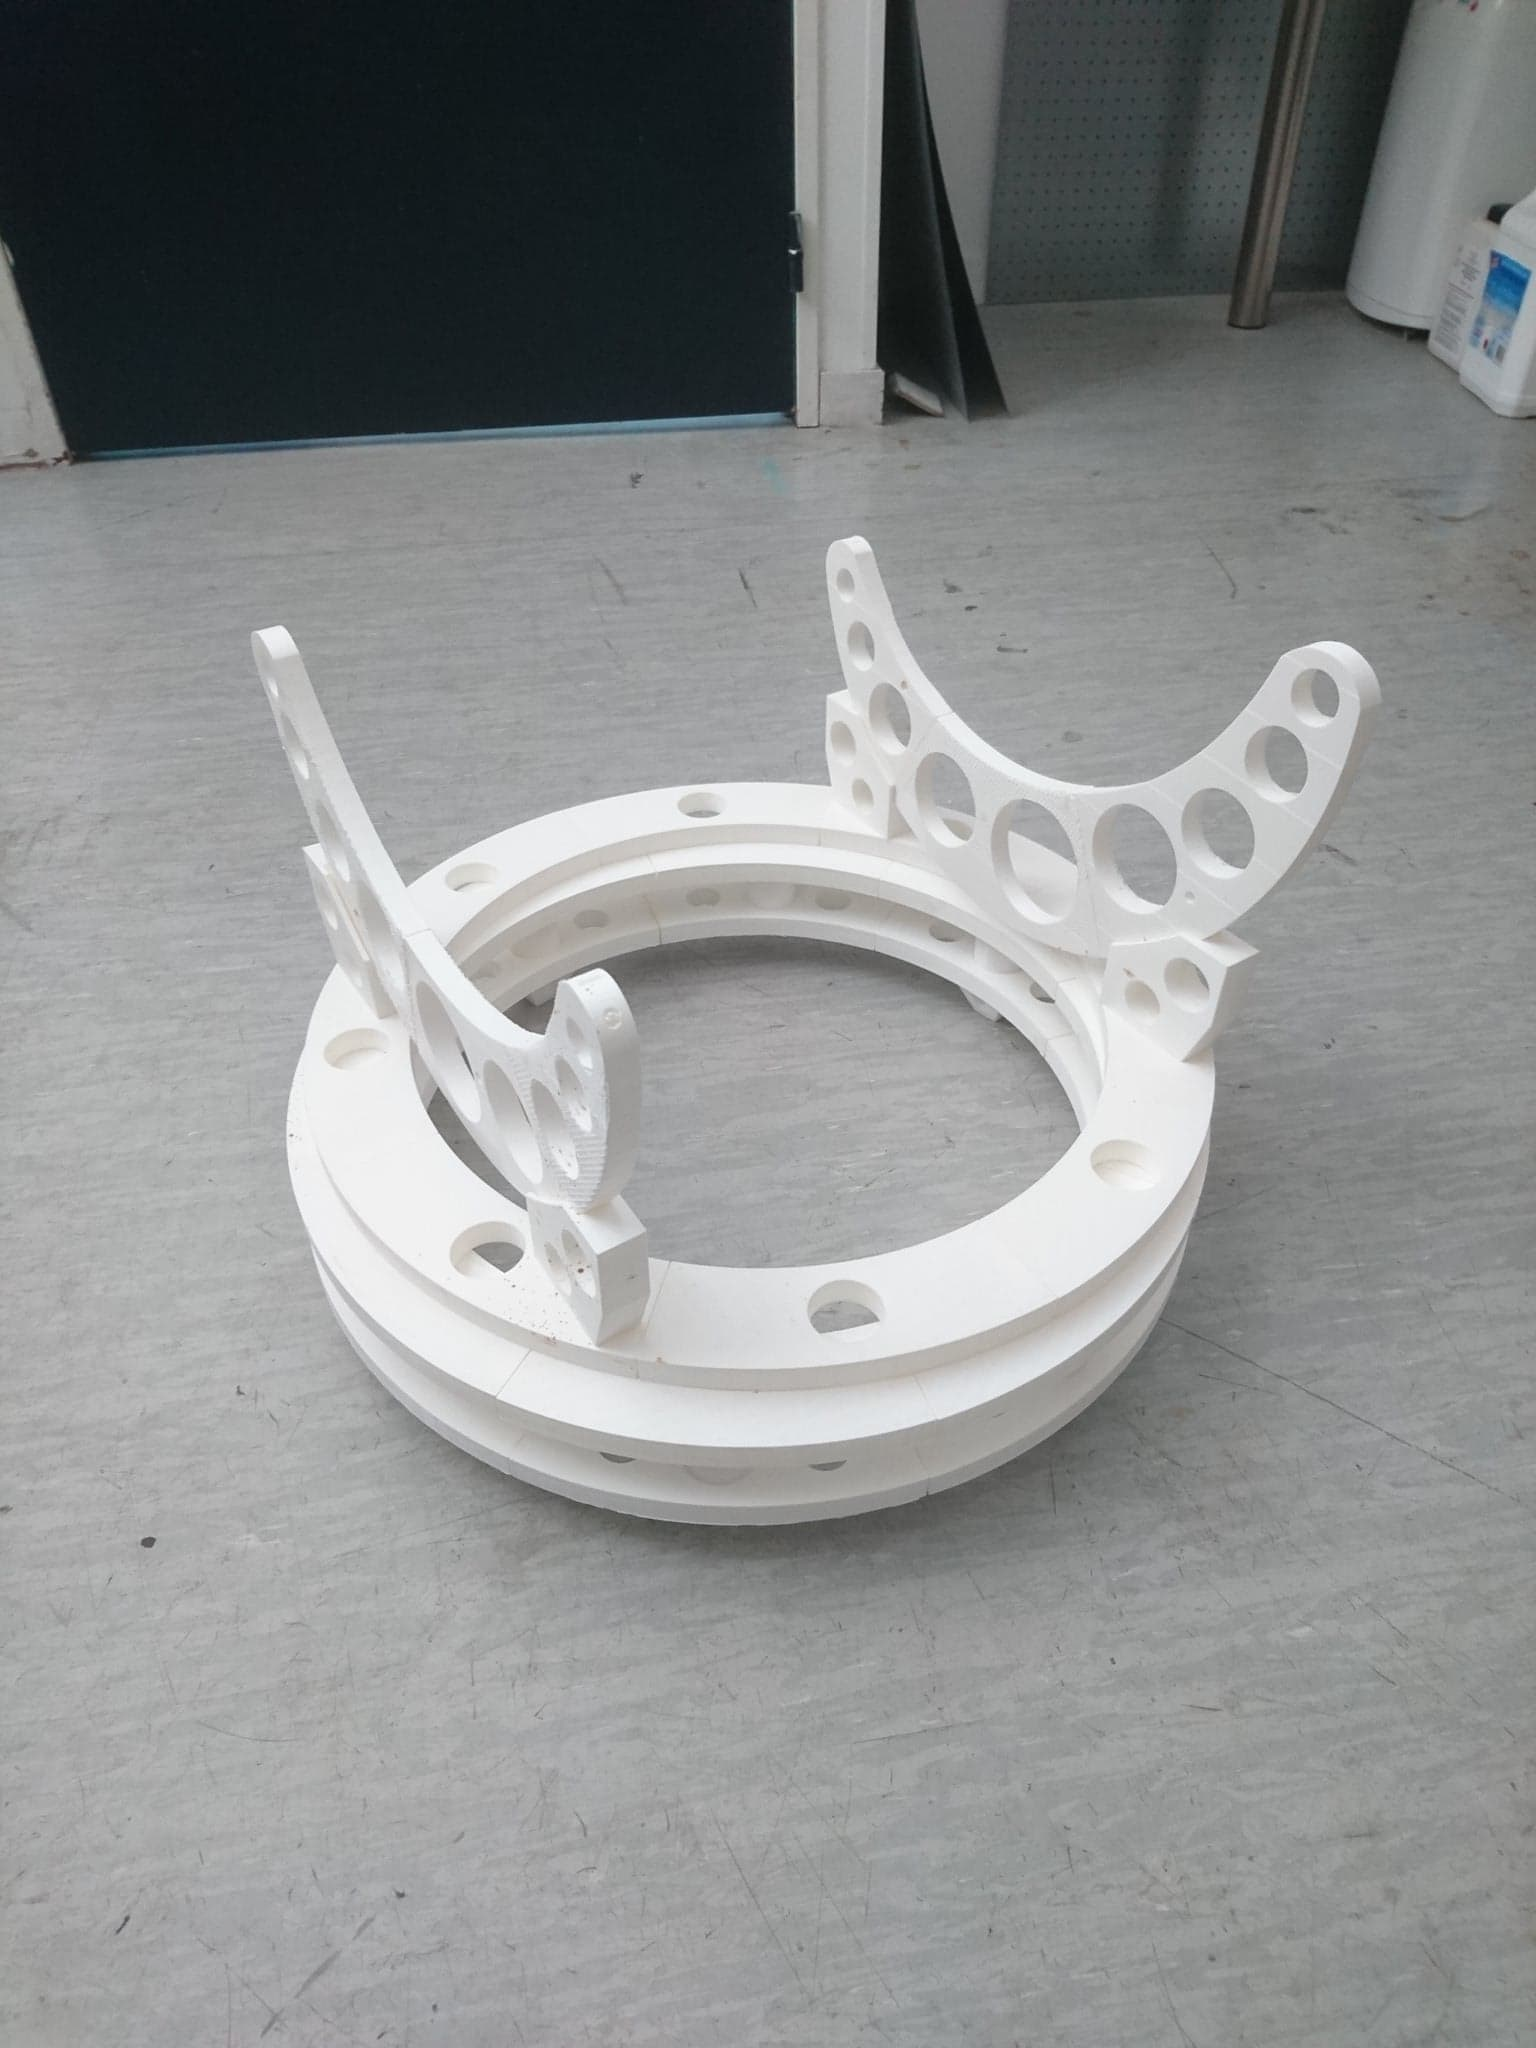
\includegraphics[width=0.3\linewidth]{\figures/photo_structure1.jpg}
    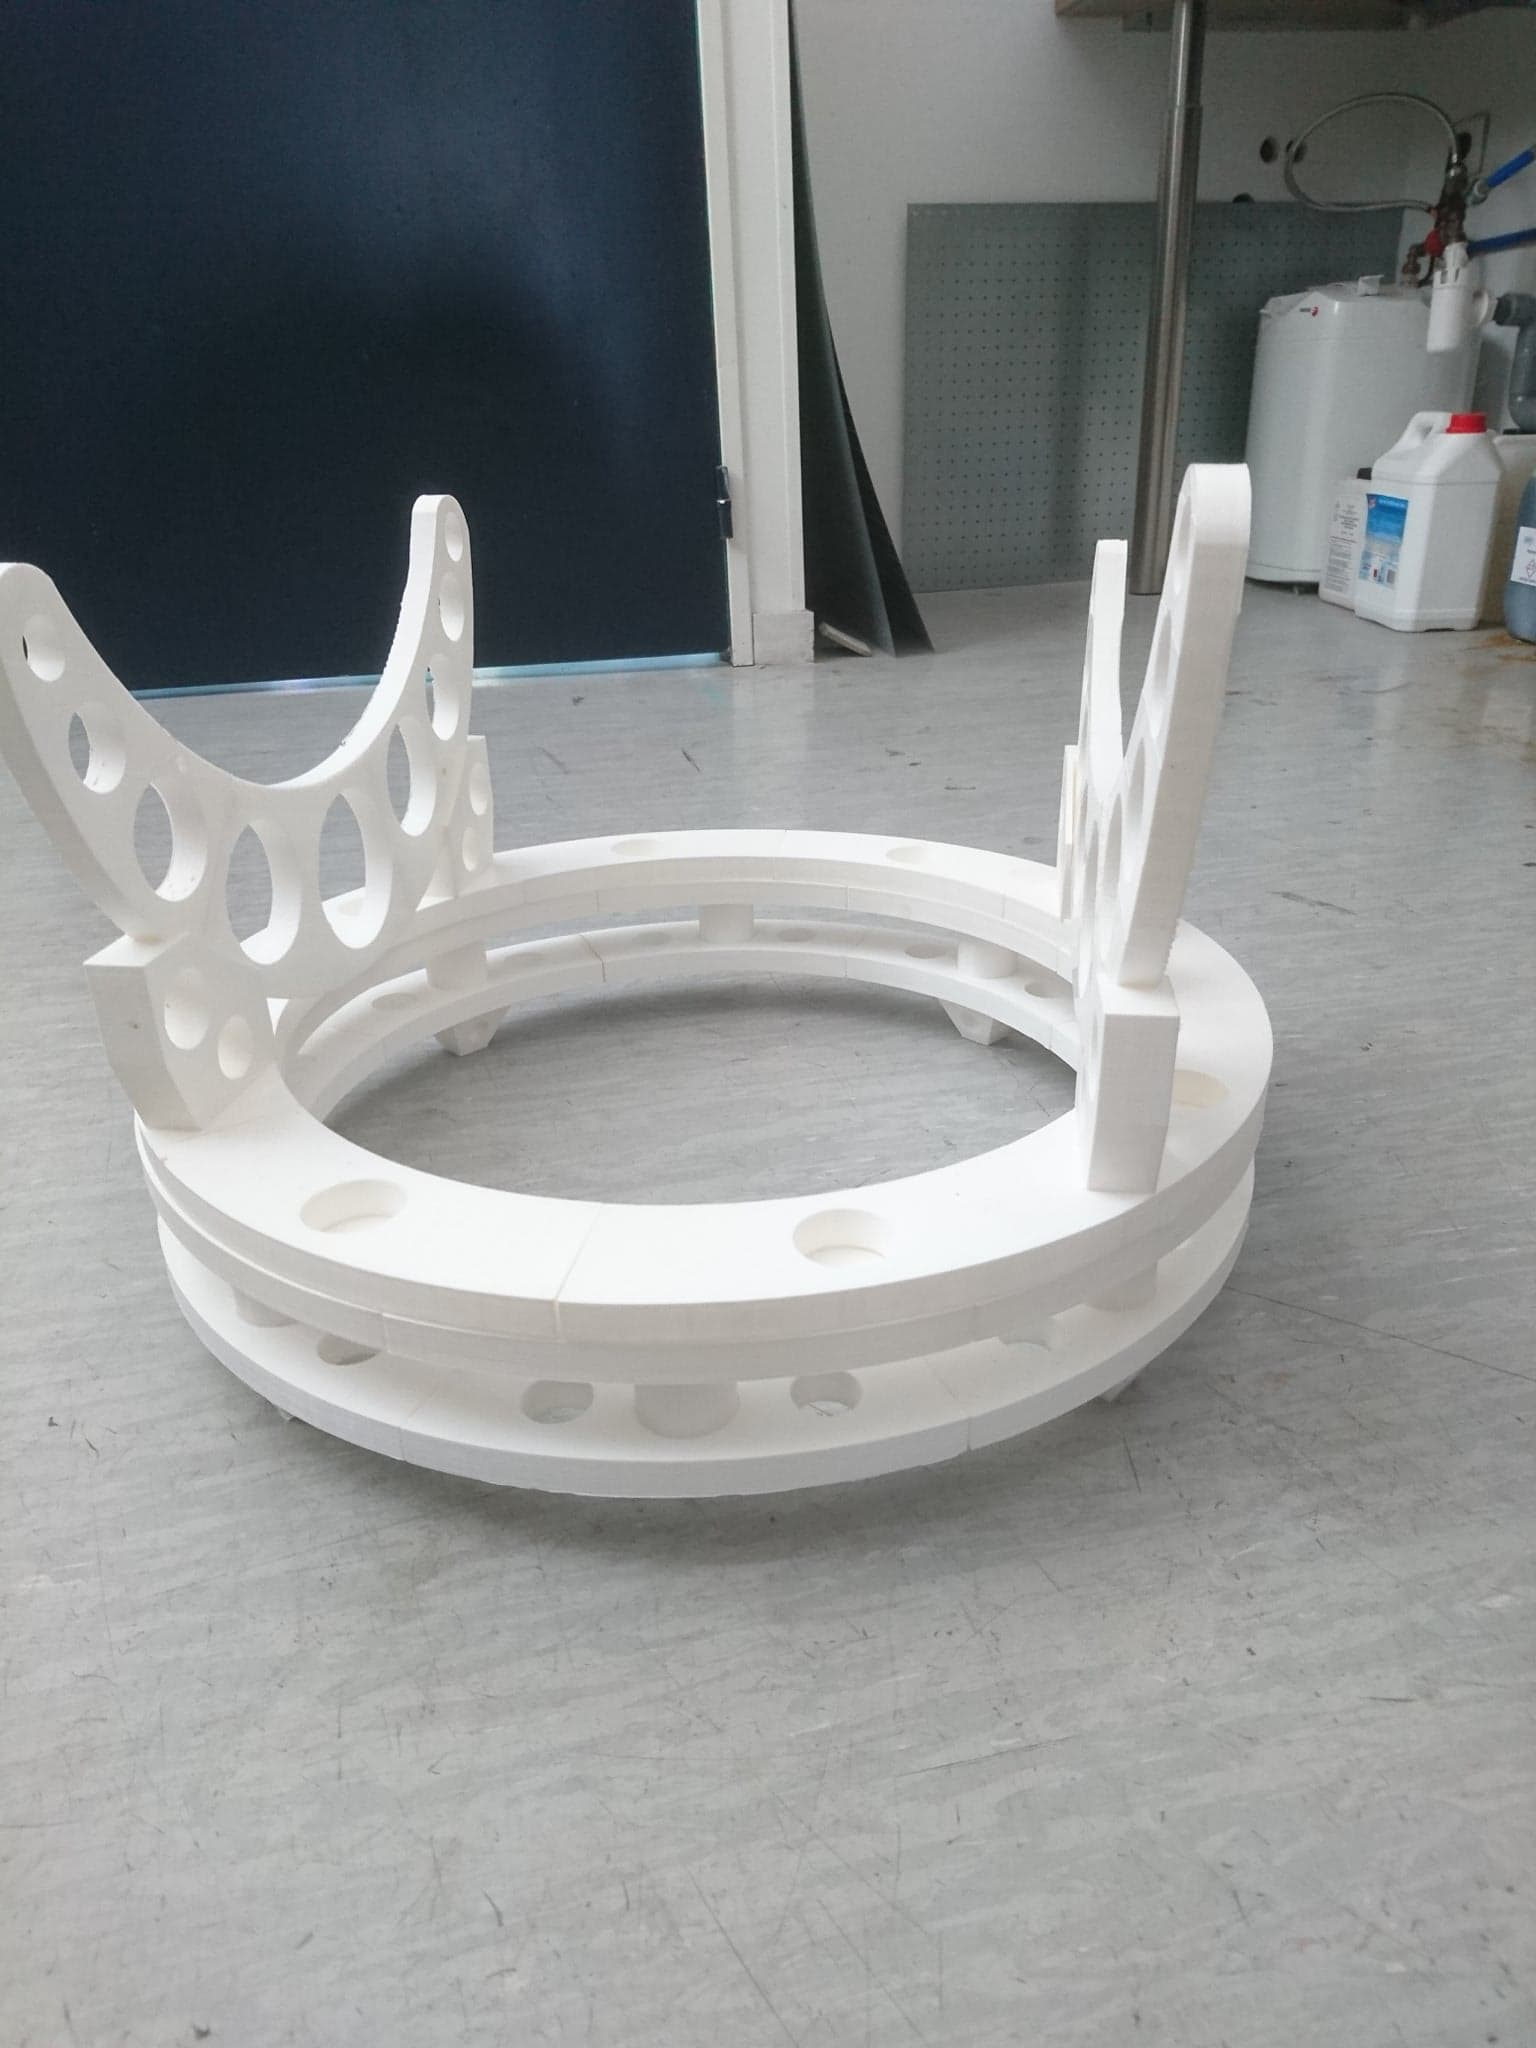
\includegraphics[width=0.3\linewidth]{\figures/photo_structure2.jpg}
    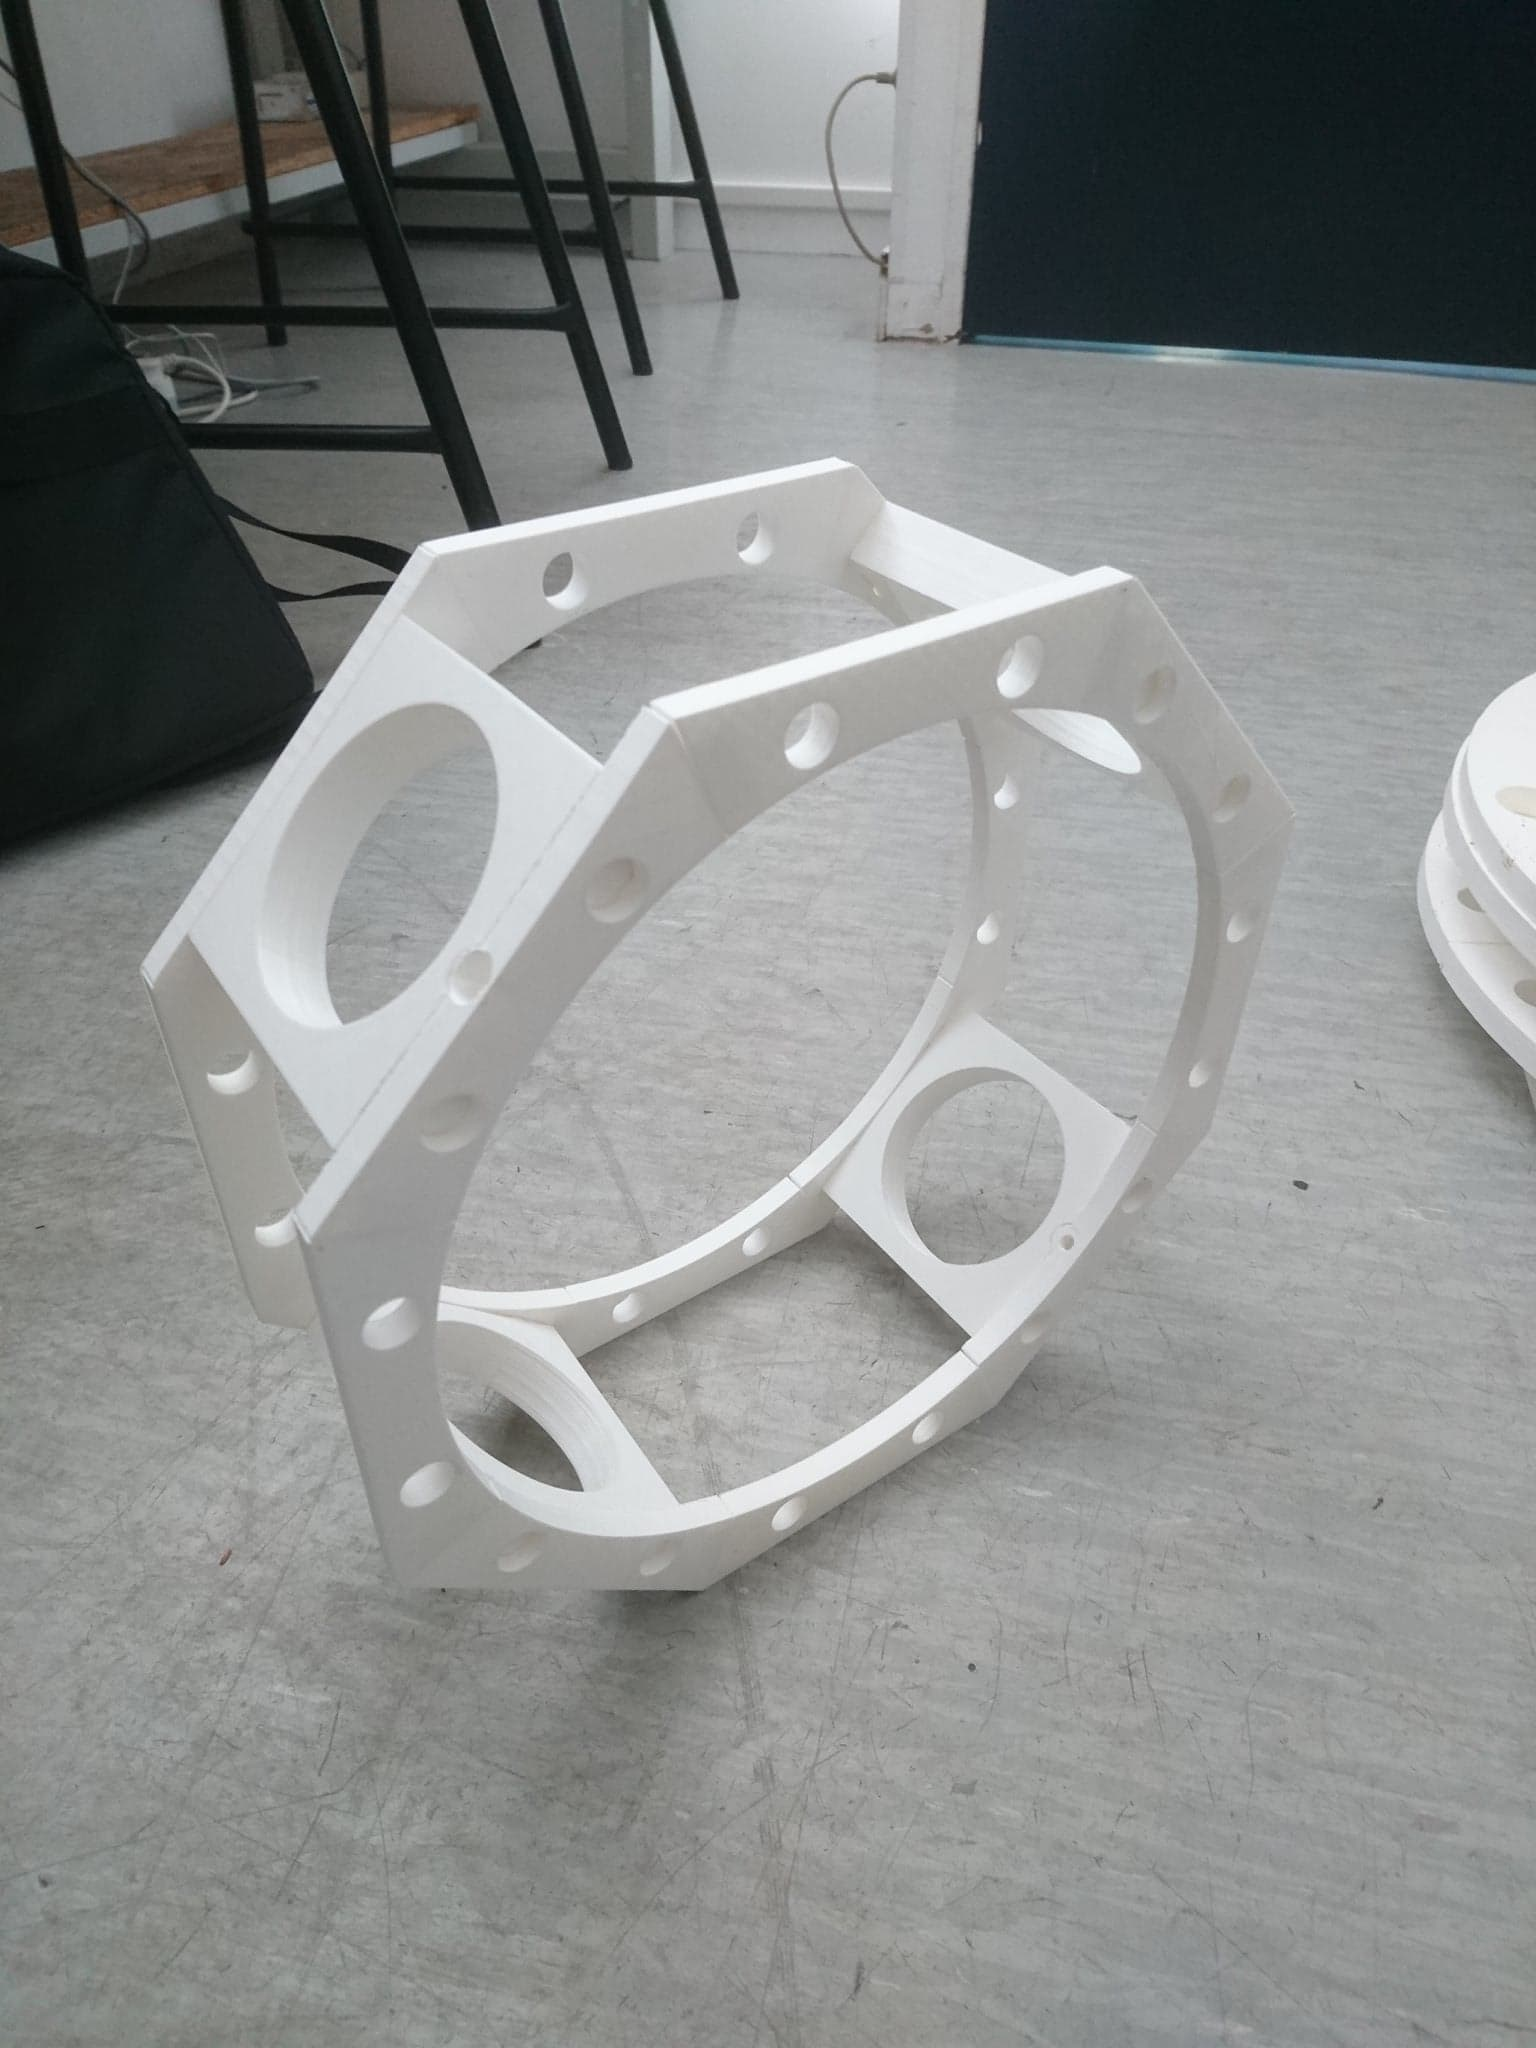
\includegraphics[width=0.3\linewidth]{\figures/photo_structure3.jpg}
    \decoRule
    \caption[
    Photos des parties montées du télescope]{
    Photos des parties montées du télescope}
    \label{fig:Photos des parties montées du télescope}
    \end{figure}


%\part{Clément AILLOUD}
%\chapter{Avancement général}

En raison de l'abandon du projet par Thibaud LE DOLEDEC et Clément AILLOUD partis en stage, le projet ne pourra être mené à terme. Pour aborder la dernière ligne droite avant l'évaluation finale, un choix a donc été fait des taches sur lesquelles travailler en priorité, au détriment d'autres qui demeureront inachevées.

\vspace{1cm}

Ci-dessous un diagramme représentant l’avancement des différentes taches du projet. Le gris indique qu’une tache est terminée ou à un niveau d’avancement satisfaisant et garantissant une maturité proche. Le orange indique les taches sur lesquelles nous travaillerons en priorité avant la fin du projet. Les flèches représentent des liens de dépendance entre les taches.

\begin{figure}[H]
    \centering
	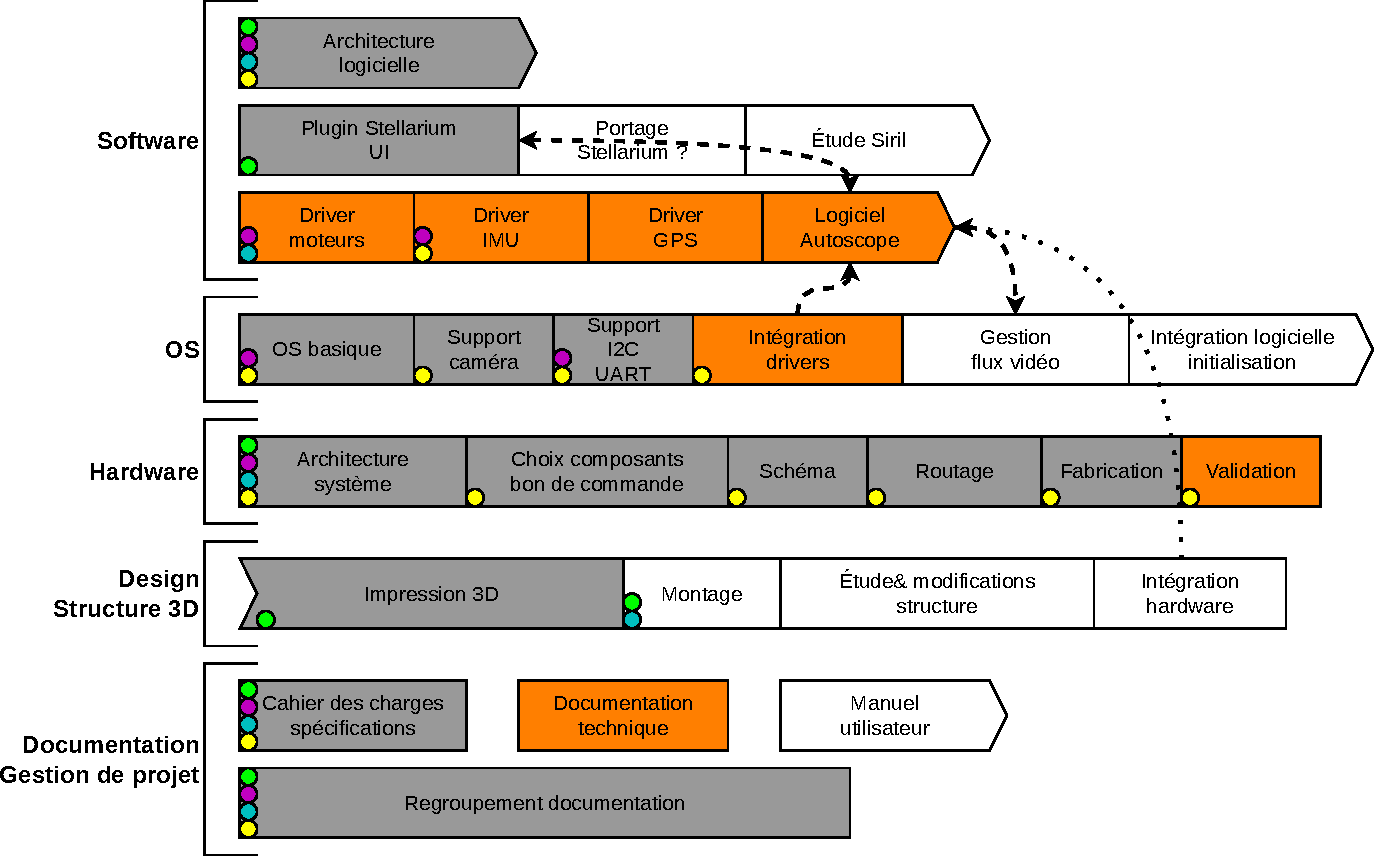
\includegraphics[width=1\linewidth]{\figures/sch_gantt.pdf}
    \decoRule
    \caption[
    Diagramme de l'organisation temporelle du travail sur le projet]{
    Diagramme de l'organisation temporelle du travail sur le projet}
    \label{fig:Diagramme de l'organisation temporelle du travail sur le projet}
    \end{figure}

\section{Prévisions pour le dernier sprint}

Malgré son aspect visuel intéressant pour promouvoir le projet ainsi que de sont aspect central (il s'agit tout de même d'un télescope), le travail sur la structure du télescope sera écarté des taches prioritaires. Cela pour deux raisons~:
\begin{itemize}[label=$\bullet$]
	\item Il s'agit d'une partie du projet demandant beaucoup de temps et d'implications par rapport à ce dont nous disposons. Nous n'aurions sans doute pas le temps de terminer cela avant l'évaluation.
	\item N'ayant ni des connaissances particulières en optique, ni la maîtrise d'un logiciel de modélisation 3D, nous ne sommes pas plus qualifiés qu'une personne aléatoire voulant contribuer au projet. Nous pensons donc qu'il vaut mieux nous concentrer sur des taches faisant partie de notre domaine de qualification, que nous serions capable de réaliser plus facilement ou mieux qu'une personne aléatoire. L'élaboration des drivers correspond typiquement à ce cas.
	\end{itemize}

\vspace{1cm}

Le travail sur les drivers, quant à lui devra être avancé autant que faire se peut. En effet le logiciel principal du télescope dépend lourdement des interfaces avec les drivers et ne peut être commencé tant que les drivers ne sont pas fonctionnels.

De plus, ce logiciel étant la clef de voûte du projet, la finalisation de certaines taches comme certains éléments du plugin Stellarium ou la gestion du flux vidéo au sein de l'OS doit être réalisée conjointement à l'écriture de ce logiciel.

L'absence des ces drivers commence donc à bloquer l'évolution d'autres taches.

\vspace{1cm}

Enfin un travail de documentation devra être fait pour qu'il soit possible à une personne future (nous-mêmes ou qui que ce soit) de travailler sur ce projet ou de réutiliser notre travail.






\appendix

%\include{Appendices/AppendixA}

\end{document}
